\documentclass[twoside]{book}

% Packages required by doxygen
\usepackage{calc}
\usepackage{doxygen}
\usepackage{graphicx}
\usepackage[utf8]{inputenc}
\usepackage{makeidx}
\usepackage{multicol}
\usepackage{multirow}
\usepackage{textcomp}
\usepackage[table]{xcolor}

% Font selection
\usepackage[T1]{fontenc}
\usepackage{mathptmx}
\usepackage[scaled=.90]{helvet}
\usepackage{courier}
\usepackage{amssymb}
\usepackage{sectsty}
\renewcommand{\familydefault}{\sfdefault}
\allsectionsfont{%
  \fontseries{bc}\selectfont%
  \color{darkgray}%
}
\renewcommand{\DoxyLabelFont}{%
  \fontseries{bc}\selectfont%
  \color{darkgray}%
}

% Page & text layout
\usepackage{geometry}
\geometry{%
  a4paper,%
  top=2.5cm,%
  bottom=2.5cm,%
  left=2.5cm,%
  right=2.5cm%
}
\tolerance=750
\hfuzz=15pt
\hbadness=750
\setlength{\emergencystretch}{15pt}
\setlength{\parindent}{0cm}
\setlength{\parskip}{0.2cm}
\makeatletter
\renewcommand{\paragraph}{%
  \@startsection{paragraph}{4}{0ex}{-1.0ex}{1.0ex}{%
    \normalfont\normalsize\bfseries\SS@parafont%
  }%
}
\renewcommand{\subparagraph}{%
  \@startsection{subparagraph}{5}{0ex}{-1.0ex}{1.0ex}{%
    \normalfont\normalsize\bfseries\SS@subparafont%
  }%
}
\makeatother

% Headers & footers
\usepackage{fancyhdr}
\pagestyle{fancyplain}
\fancyhead[LE]{\fancyplain{}{\bfseries\thepage}}
\fancyhead[CE]{\fancyplain{}{}}
\fancyhead[RE]{\fancyplain{}{\bfseries\leftmark}}
\fancyhead[LO]{\fancyplain{}{\bfseries\rightmark}}
\fancyhead[CO]{\fancyplain{}{}}
\fancyhead[RO]{\fancyplain{}{\bfseries\thepage}}
\fancyfoot[LE]{\fancyplain{}{}}
\fancyfoot[CE]{\fancyplain{}{}}
\fancyfoot[RE]{\fancyplain{}{\bfseries\scriptsize Generated on Mon Nov 9 2015 19\-:16\-:58 for Multilevel Prediction by Doxygen }}
\fancyfoot[LO]{\fancyplain{}{\bfseries\scriptsize Generated on Mon Nov 9 2015 19\-:16\-:58 for Multilevel Prediction by Doxygen }}
\fancyfoot[CO]{\fancyplain{}{}}
\fancyfoot[RO]{\fancyplain{}{}}
\renewcommand{\footrulewidth}{0.4pt}
\renewcommand{\chaptermark}[1]{%
  \markboth{#1}{}%
}
\renewcommand{\sectionmark}[1]{%
  \markright{\thesection\ #1}%
}

% Indices & bibliography
\usepackage{natbib}
\usepackage[titles]{tocloft}
\setcounter{tocdepth}{3}
\setcounter{secnumdepth}{5}
\makeindex

% Hyperlinks (required, but should be loaded last)
\usepackage{ifpdf}
\ifpdf
  \usepackage[pdftex,pagebackref=true]{hyperref}
\else
  \usepackage[ps2pdf,pagebackref=true]{hyperref}
\fi
\hypersetup{%
  colorlinks=true,%
  linkcolor=blue,%
  citecolor=blue,%
  unicode%
}

% Custom commands
\newcommand{\clearemptydoublepage}{%
  \newpage{\pagestyle{empty}\cleardoublepage}%
}


%===== C O N T E N T S =====

\begin{document}

% Titlepage & ToC
\hypersetup{pageanchor=false}
\pagenumbering{roman}
\begin{titlepage}
\vspace*{7cm}
\begin{center}%
{\Large Multilevel Prediction }\\
\vspace*{1cm}
{\large Generated by Doxygen 1.8.6}\\
\vspace*{0.5cm}
{\small Mon Nov 9 2015 19:16:58}\\
\end{center}
\end{titlepage}
\clearemptydoublepage
\tableofcontents
\clearemptydoublepage
\pagenumbering{arabic}
\hypersetup{pageanchor=true}

%--- Begin generated contents ---
\chapter{Main Page}
\label{index}\hypertarget{index}{}This program is a toolbox to compute optimal predictors of Markov chains, and in particular multilevel agent-\/based systems, by using the information bottleneck method. For details regarding the formal grounds of this method, please refer to\-:

Robin Lamarche-\/\-Perrin, Sven Banisch, and Eckehard Olbrich. The Information Bottleneck Method for Optimal Prediction of Multilevel Agent-\/based Systems. Technical Report M\-I\-S-\/\-Preprint 55/2015, Max Planck Institute for Mathematics in the Sciences, Leipzig, Germany, 2015.

\href{http://www.mis.mpg.de/publications/preprints/2015/prepr2015-55.html}{\tt http\-://www.\-mis.\-mpg.\-de/publications/preprints/2015/prepr2015-\/55.\-html}

Copyright © 2015 Robin Lamarche-\/\-Perrin (\href{mailto:Robin.Lamarche-Perrin@lip6.fr}{\tt Robin.\-Lamarche-\/\-Perrin@lip6.\-fr})

This program is free software\-: you can redistribute it and/or modify it under the terms of the G\-N\-U General Public License as published by the Free Software Foundation, either version 3 of the License, or (at your option) any later version.

This program is distributed in the hope that it will be useful, but W\-I\-T\-H\-O\-U\-T A\-N\-Y W\-A\-R\-R\-A\-N\-T\-Y; without even the implied warranty of M\-E\-R\-C\-H\-A\-N\-T\-A\-B\-I\-L\-I\-T\-Y or F\-I\-T\-N\-E\-S\-S F\-O\-R A P\-A\-R\-T\-I\-C\-U\-L\-A\-R P\-U\-R\-P\-O\-S\-E. See the G\-N\-U General Public License for more details.

You should have received a copy of the G\-N\-U General Public License along with this program. If not, see \href{http://www.gnu.org/licenses/}{\tt http\-://www.\-gnu.\-org/licenses/}. 
\chapter{Hierarchical Index}
\section{Class Hierarchy}
This inheritance list is sorted roughly, but not completely, alphabetically\-:\begin{DoxyCompactList}
\item \contentsline{section}{Chain\-Experiment}{\pageref{class_chain_experiment}}{}
\item \contentsline{section}{Data\-Point\-Struct}{\pageref{struct_data_point_struct}}{}
\item \contentsline{section}{Markov\-Data\-Set}{\pageref{class_markov_data_set}}{}
\item \contentsline{section}{Markov\-Process}{\pageref{class_markov_process}}{}
\item \contentsline{section}{Markov\-Trajectory}{\pageref{class_markov_trajectory}}{}
\item \contentsline{section}{Ordered\-Partition}{\pageref{class_ordered_partition}}{}
\item \contentsline{section}{Part}{\pageref{class_part}}{}
\item \contentsline{section}{Partition}{\pageref{class_partition}}{}
\item \contentsline{section}{Timer}{\pageref{class_timer}}{}
\item \contentsline{section}{Two\-Communities\-Experiment}{\pageref{class_two_communities_experiment}}{}
\item \contentsline{section}{Voter\-Binning}{\pageref{class_voter_binning}}{}
\item \contentsline{section}{Voter\-Data\-Set}{\pageref{class_voter_data_set}}{}
\item \contentsline{section}{Voter\-Edge}{\pageref{class_voter_edge}}{}
\item \contentsline{section}{Voter\-Graph}{\pageref{class_voter_graph}}{}
\begin{DoxyCompactList}
\item \contentsline{section}{Chain\-Voter\-Graph}{\pageref{class_chain_voter_graph}}{}
\item \contentsline{section}{Complete\-Voter\-Graph}{\pageref{class_complete_voter_graph}}{}
\item \contentsline{section}{Two\-Communities\-Voter\-Graph}{\pageref{class_two_communities_voter_graph}}{}
\end{DoxyCompactList}
\item \contentsline{section}{Voter\-Measurement}{\pageref{class_voter_measurement}}{}
\begin{DoxyCompactList}
\item \contentsline{section}{Empty\-Voter\-Measurement}{\pageref{class_empty_voter_measurement}}{}
\item \contentsline{section}{Macro\-Voter\-Measurement}{\pageref{class_macro_voter_measurement}}{}
\item \contentsline{section}{Micro\-Voter\-Measurement}{\pageref{class_micro_voter_measurement}}{}
\end{DoxyCompactList}
\item \contentsline{section}{Voter\-Measurement\-State}{\pageref{class_voter_measurement_state}}{}
\item \contentsline{section}{Voter\-Measurement\-Trajectory}{\pageref{class_voter_measurement_trajectory}}{}
\item \contentsline{section}{Voter\-Node}{\pageref{class_voter_node}}{}
\item \contentsline{section}{Voter\-Probe}{\pageref{class_voter_probe}}{}
\item \contentsline{section}{Voter\-State}{\pageref{class_voter_state}}{}
\item \contentsline{section}{Voter\-Trajectory}{\pageref{class_voter_trajectory}}{}
\end{DoxyCompactList}

\chapter{Class Index}
\section{Class List}
Here are the classes, structs, unions and interfaces with brief descriptions\+:\begin{DoxyCompactList}
\item\contentsline{section}{\hyperlink{class_complete_voter_graph}{Complete\+Voter\+Graph} \\*An interaction graph with edges between each pair of nodes (in both direction, with equal weight for each edge) }{\pageref{class_complete_voter_graph}}{}
\item\contentsline{section}{\hyperlink{struct_data_point_struct}{Data\+Point\+Struct} \\*The computation time and memory consumption associated to an experiment of a given size }{\pageref{struct_data_point_struct}}{}
\item\contentsline{section}{\hyperlink{class_empty_voter_measurement}{Empty\+Voter\+Measurement} \\*A measurement without any probe (no observation) }{\pageref{class_empty_voter_measurement}}{}
\item\contentsline{section}{\hyperlink{class_macro_voter_measurement}{Macro\+Voter\+Measurement} \\*A measurement consisting in one probe observing all nodes of the interaction graph }{\pageref{class_macro_voter_measurement}}{}
\item\contentsline{section}{\hyperlink{class_markov_process}{Markov\+Process} \\*A finite Markov chain described by a discrete state space, an initial distribution, and a transition kernel }{\pageref{class_markov_process}}{}
\item\contentsline{section}{\hyperlink{class_micro_voter_measurement}{Micro\+Voter\+Measurement} \\*A measurement consisting in one probe for each node of the interaction graph }{\pageref{class_micro_voter_measurement}}{}
\item\contentsline{section}{\hyperlink{class_part}{Part} \\*A part of a partition (i.\+e., a set of individuals) }{\pageref{class_part}}{}
\item\contentsline{section}{\hyperlink{class_partition}{Partition} \\*A partition (i.\+e., a set of disjoint and covering parts) }{\pageref{class_partition}}{}
\item\contentsline{section}{\hyperlink{class_timer}{Timer} \\*A timer mesuring computation times and memory consumption during the program execution }{\pageref{class_timer}}{}
\item\contentsline{section}{\hyperlink{class_two_communities_voter_graph}{Two\+Communities\+Voter\+Graph} \\*An interaction graph consisting in two communities of nodes (complete graph within each community, complete interaction between the two communities, possibly with different weights) }{\pageref{class_two_communities_voter_graph}}{}
\item\contentsline{section}{\hyperlink{class_voter_edge}{Voter\+Edge} \\*An edge of the interaction graph }{\pageref{class_voter_edge}}{}
\item\contentsline{section}{\hyperlink{class_voter_experiment}{Voter\+Experiment} \\*Programming a prediction experiment on a two-\/communities Voter Model }{\pageref{class_voter_experiment}}{}
\item\contentsline{section}{\hyperlink{class_voter_graph}{Voter\+Graph} \\*The interaction graph describing a Voter Model }{\pageref{class_voter_graph}}{}
\item\contentsline{section}{\hyperlink{class_voter_measurement}{Voter\+Measurement} \\*A measurement to observe the Voter Model according set of probes }{\pageref{class_voter_measurement}}{}
\item\contentsline{section}{\hyperlink{class_voter_node}{Voter\+Node} \\*A node of the interaction graph }{\pageref{class_voter_node}}{}
\item\contentsline{section}{\hyperlink{class_voter_probe}{Voter\+Probe} \\*A probe to observe the Voter Model according to a subset of nodes }{\pageref{class_voter_probe}}{}
\end{DoxyCompactList}

\chapter{File Index}
\section{File List}
Here is a list of all documented files with brief descriptions\-:\begin{DoxyCompactList}
\item\contentsline{section}{/home/lamarche/programming/multilevel\-\_\-prediction/src/{\bfseries coconut.\-hpp} }{\pageref{coconut_8hpp}}{}
\item\contentsline{section}{/home/lamarche/programming/multilevel\-\_\-prediction/src/\hyperlink{csv__tools_8hpp}{csv\-\_\-tools.\-hpp} \\*Tools to handle input and output C\-S\-V files }{\pageref{csv__tools_8hpp}}{}
\item\contentsline{section}{/home/lamarche/programming/multilevel\-\_\-prediction/src/{\bfseries landuse.\-hpp} }{\pageref{landuse_8hpp}}{}
\item\contentsline{section}{/home/lamarche/programming/multilevel\-\_\-prediction/src/\hyperlink{main_8hpp}{main.\-hpp} \\*Main program to run tests and experiments (see for example class Voter\-Experiment) }{\pageref{main_8hpp}}{}
\item\contentsline{section}{/home/lamarche/programming/multilevel\-\_\-prediction/src/\hyperlink{markov__process_8hpp}{markov\-\_\-process.\-hpp} \\*Class to build a finite Markov chain }{\pageref{markov__process_8hpp}}{}
\item\contentsline{section}{/home/lamarche/programming/multilevel\-\_\-prediction/src/\hyperlink{partition_8hpp}{partition.\-hpp} \\*Classes to build partitions of the state space of Markov chains }{\pageref{partition_8hpp}}{}
\item\contentsline{section}{/home/lamarche/programming/multilevel\-\_\-prediction/src/\hyperlink{timer_8hpp}{timer.\-hpp} \\*Tools to mesure computation times and memory consumption during the program execution }{\pageref{timer_8hpp}}{}
\item\contentsline{section}{/home/lamarche/programming/multilevel\-\_\-prediction/src/\hyperlink{voter__experiment_8hpp}{voter\-\_\-experiment.\-hpp} \\*Tools to run prediction experiments on Voter Models }{\pageref{voter__experiment_8hpp}}{}
\item\contentsline{section}{/home/lamarche/programming/multilevel\-\_\-prediction/src/\hyperlink{voter__graph_8hpp}{voter\-\_\-graph.\-hpp} \\*Classes to build an interaction graph (nodes and edges) describing a Voter Model and some observation tools (probes and measurements) }{\pageref{voter__graph_8hpp}}{}
\end{DoxyCompactList}

\chapter{Class Documentation}
\hypertarget{class_chain_experiment}{\section{Chain\-Experiment Class Reference}
\label{class_chain_experiment}\index{Chain\-Experiment@{Chain\-Experiment}}
}
\subsection*{Public Member Functions}
\begin{DoxyCompactItemize}
\item 
\hypertarget{class_chain_experiment_a0abdddd54c8d25e68b9e372b10c818b4}{{\bfseries Chain\-Experiment} (int size, double contrarian, bool ring, double time, double delay, Spec\-Measurement\-Set $\ast$\hyperlink{class_chain_experiment_adbc54d1d7cd2d86f838b0128e5597216}{pre\-Measurements}, Spec\-Measurement\-Set $\ast$\hyperlink{class_chain_experiment_a9362d54e02df4c8dd2a461b7aa4e322a}{post\-Measurements})}\label{class_chain_experiment_a0abdddd54c8d25e68b9e372b10c818b4}

\end{DoxyCompactItemize}
\subsection*{Public Attributes}
\begin{DoxyCompactItemize}
\item 
int \hyperlink{class_chain_experiment_ab197887e94e2586b3ba274bef7211c8c}{id}
\item 
\hyperlink{voter__graph_8hpp_ab3bec55c359e4ed771339c8bc61fc35a}{Update\-Process} \hyperlink{class_chain_experiment_a31b4dac82ed978b8ccad094496346fde}{update}
\item 
double \hyperlink{class_chain_experiment_ac17a3b382a5301adb5139fbaf8d53f49}{threshold}
\item 
\hypertarget{class_chain_experiment_abe6348bf4159c619989cd7ab6cfc60ec}{bool {\bfseries with\-Aggregation}}\label{class_chain_experiment_abe6348bf4159c619989cd7ab6cfc60ec}

\item 
\hypertarget{class_chain_experiment_ad5030f61a3cb618deefa33508ecb18de}{bool {\bfseries ring}}\label{class_chain_experiment_ad5030f61a3cb618deefa33508ecb18de}

\item 
\hypertarget{class_chain_experiment_a7b2e6eef6dd5e4b761b048ce07c72f46}{int {\bfseries size\-Min}}\label{class_chain_experiment_a7b2e6eef6dd5e4b761b048ce07c72f46}

\item 
\hypertarget{class_chain_experiment_ad6cecf9ed170262ac9f9579b5c6dd8b1}{int {\bfseries size\-Max}}\label{class_chain_experiment_ad6cecf9ed170262ac9f9579b5c6dd8b1}

\item 
\hypertarget{class_chain_experiment_a08edc0b2dd722042534cec3b3814b737}{int {\bfseries size\-Step}}\label{class_chain_experiment_a08edc0b2dd722042534cec3b3814b737}

\item 
double \hyperlink{class_chain_experiment_a343f957d771934c6bada7613c020c07f}{contrarian\-Min}
\item 
double \hyperlink{class_chain_experiment_a02ea31bc14bc89d32fba19ed3439ad3f}{contrarian\-Max}
\item 
double \hyperlink{class_chain_experiment_a072bef3805353ee08e7ac3b8e4d8d69b}{contrarian\-Step}
\item 
int \hyperlink{class_chain_experiment_a92b1a39b84c5d3f2642db40b951e4582}{time\-Min}
\item 
int \hyperlink{class_chain_experiment_a9d7233a2ba46450f3ff10494100f21b9}{time\-Max}
\item 
int \hyperlink{class_chain_experiment_a5be9b1c06782e8e8e365080bca05e61d}{time\-Step}
\item 
int \hyperlink{class_chain_experiment_a06dd6bc7fbeeb3d6a0f506e7e239240c}{delay\-Min}
\item 
int \hyperlink{class_chain_experiment_aece190c28fdde383004c31a75be5166a}{delay\-Max}
\item 
int \hyperlink{class_chain_experiment_ada234ba1f0da4c9f2828ac759d1c7c4f}{delay\-Step}
\item 
Spec\-Measurement\-Set $\ast$ \hyperlink{class_chain_experiment_adbc54d1d7cd2d86f838b0128e5597216}{pre\-Measurements}
\item 
Spec\-Measurement\-Set $\ast$ \hyperlink{class_chain_experiment_a9362d54e02df4c8dd2a461b7aa4e322a}{post\-Measurements}
\end{DoxyCompactItemize}
\subsection*{Static Public Attributes}
\begin{DoxyCompactItemize}
\item 
\hypertarget{class_chain_experiment_a1691a5dc572e94812033e06156995362}{static int {\bfseries id\-\_\-number} = 0}\label{class_chain_experiment_a1691a5dc572e94812033e06156995362}

\end{DoxyCompactItemize}


\subsection{Member Data Documentation}
\hypertarget{class_chain_experiment_a02ea31bc14bc89d32fba19ed3439ad3f}{\index{Chain\-Experiment@{Chain\-Experiment}!contrarian\-Max@{contrarian\-Max}}
\index{contrarian\-Max@{contrarian\-Max}!ChainExperiment@{Chain\-Experiment}}
\subsubsection[{contrarian\-Max}]{\setlength{\rightskip}{0pt plus 5cm}double Chain\-Experiment\-::contrarian\-Max}}\label{class_chain_experiment_a02ea31bc14bc89d32fba19ed3439ad3f}
The contrarian rate of nodes within community 1 in the last experiment \hypertarget{class_chain_experiment_a343f957d771934c6bada7613c020c07f}{\index{Chain\-Experiment@{Chain\-Experiment}!contrarian\-Min@{contrarian\-Min}}
\index{contrarian\-Min@{contrarian\-Min}!ChainExperiment@{Chain\-Experiment}}
\subsubsection[{contrarian\-Min}]{\setlength{\rightskip}{0pt plus 5cm}double Chain\-Experiment\-::contrarian\-Min}}\label{class_chain_experiment_a343f957d771934c6bada7613c020c07f}
The contrarian rate of nodes within community 1 in the first experiment \hypertarget{class_chain_experiment_a072bef3805353ee08e7ac3b8e4d8d69b}{\index{Chain\-Experiment@{Chain\-Experiment}!contrarian\-Step@{contrarian\-Step}}
\index{contrarian\-Step@{contrarian\-Step}!ChainExperiment@{Chain\-Experiment}}
\subsubsection[{contrarian\-Step}]{\setlength{\rightskip}{0pt plus 5cm}double Chain\-Experiment\-::contrarian\-Step}}\label{class_chain_experiment_a072bef3805353ee08e7ac3b8e4d8d69b}
The contrarian rate of nodes within community 1 between two consecutive experiments \hypertarget{class_chain_experiment_aece190c28fdde383004c31a75be5166a}{\index{Chain\-Experiment@{Chain\-Experiment}!delay\-Max@{delay\-Max}}
\index{delay\-Max@{delay\-Max}!ChainExperiment@{Chain\-Experiment}}
\subsubsection[{delay\-Max}]{\setlength{\rightskip}{0pt plus 5cm}int Chain\-Experiment\-::delay\-Max}}\label{class_chain_experiment_aece190c28fdde383004c31a75be5166a}
The delay before post-\/measurement in the last experiment \hypertarget{class_chain_experiment_a06dd6bc7fbeeb3d6a0f506e7e239240c}{\index{Chain\-Experiment@{Chain\-Experiment}!delay\-Min@{delay\-Min}}
\index{delay\-Min@{delay\-Min}!ChainExperiment@{Chain\-Experiment}}
\subsubsection[{delay\-Min}]{\setlength{\rightskip}{0pt plus 5cm}int Chain\-Experiment\-::delay\-Min}}\label{class_chain_experiment_a06dd6bc7fbeeb3d6a0f506e7e239240c}
The delay before post-\/measurement in the first experiment \hypertarget{class_chain_experiment_ada234ba1f0da4c9f2828ac759d1c7c4f}{\index{Chain\-Experiment@{Chain\-Experiment}!delay\-Step@{delay\-Step}}
\index{delay\-Step@{delay\-Step}!ChainExperiment@{Chain\-Experiment}}
\subsubsection[{delay\-Step}]{\setlength{\rightskip}{0pt plus 5cm}int Chain\-Experiment\-::delay\-Step}}\label{class_chain_experiment_ada234ba1f0da4c9f2828ac759d1c7c4f}
The delay before post-\/measurement between two consecutive experiments \hypertarget{class_chain_experiment_ab197887e94e2586b3ba274bef7211c8c}{\index{Chain\-Experiment@{Chain\-Experiment}!id@{id}}
\index{id@{id}!ChainExperiment@{Chain\-Experiment}}
\subsubsection[{id}]{\setlength{\rightskip}{0pt plus 5cm}int Chain\-Experiment\-::id}}\label{class_chain_experiment_ab197887e94e2586b3ba274bef7211c8c}
A unique experiment number \hypertarget{class_chain_experiment_a9362d54e02df4c8dd2a461b7aa4e322a}{\index{Chain\-Experiment@{Chain\-Experiment}!post\-Measurements@{post\-Measurements}}
\index{post\-Measurements@{post\-Measurements}!ChainExperiment@{Chain\-Experiment}}
\subsubsection[{post\-Measurements}]{\setlength{\rightskip}{0pt plus 5cm}Spec\-Measurement\-Set$\ast$ Chain\-Experiment\-::post\-Measurements}}\label{class_chain_experiment_a9362d54e02df4c8dd2a461b7aa4e322a}
A set of post-\/measurement to be predicted \hypertarget{class_chain_experiment_adbc54d1d7cd2d86f838b0128e5597216}{\index{Chain\-Experiment@{Chain\-Experiment}!pre\-Measurements@{pre\-Measurements}}
\index{pre\-Measurements@{pre\-Measurements}!ChainExperiment@{Chain\-Experiment}}
\subsubsection[{pre\-Measurements}]{\setlength{\rightskip}{0pt plus 5cm}Spec\-Measurement\-Set$\ast$ Chain\-Experiment\-::pre\-Measurements}}\label{class_chain_experiment_adbc54d1d7cd2d86f838b0128e5597216}
A set of pre-\/measurement for prediction \hypertarget{class_chain_experiment_ac17a3b382a5301adb5139fbaf8d53f49}{\index{Chain\-Experiment@{Chain\-Experiment}!threshold@{threshold}}
\index{threshold@{threshold}!ChainExperiment@{Chain\-Experiment}}
\subsubsection[{threshold}]{\setlength{\rightskip}{0pt plus 5cm}double Chain\-Experiment\-::threshold}}\label{class_chain_experiment_ac17a3b382a5301adb5139fbaf8d53f49}
The precision threshold to compute the stationary distribution of the Markov chain (see compute\-Stationary\-Distribution method in \hyperlink{class_markov_process}{Markov\-Process} class) \hypertarget{class_chain_experiment_a9d7233a2ba46450f3ff10494100f21b9}{\index{Chain\-Experiment@{Chain\-Experiment}!time\-Max@{time\-Max}}
\index{time\-Max@{time\-Max}!ChainExperiment@{Chain\-Experiment}}
\subsubsection[{time\-Max}]{\setlength{\rightskip}{0pt plus 5cm}int Chain\-Experiment\-::time\-Max}}\label{class_chain_experiment_a9d7233a2ba46450f3ff10494100f21b9}
The time of pre-\/measurement (-\/1 for stationary distribution) in the last experiment \hypertarget{class_chain_experiment_a92b1a39b84c5d3f2642db40b951e4582}{\index{Chain\-Experiment@{Chain\-Experiment}!time\-Min@{time\-Min}}
\index{time\-Min@{time\-Min}!ChainExperiment@{Chain\-Experiment}}
\subsubsection[{time\-Min}]{\setlength{\rightskip}{0pt plus 5cm}int Chain\-Experiment\-::time\-Min}}\label{class_chain_experiment_a92b1a39b84c5d3f2642db40b951e4582}
The time of pre-\/measurement (-\/1 for stationary distribution) in the first experiment \hypertarget{class_chain_experiment_a5be9b1c06782e8e8e365080bca05e61d}{\index{Chain\-Experiment@{Chain\-Experiment}!time\-Step@{time\-Step}}
\index{time\-Step@{time\-Step}!ChainExperiment@{Chain\-Experiment}}
\subsubsection[{time\-Step}]{\setlength{\rightskip}{0pt plus 5cm}int Chain\-Experiment\-::time\-Step}}\label{class_chain_experiment_a5be9b1c06782e8e8e365080bca05e61d}
The time of pre-\/measurement (-\/1 for stationary distribution) between two consecutive experiments \hypertarget{class_chain_experiment_a31b4dac82ed978b8ccad094496346fde}{\index{Chain\-Experiment@{Chain\-Experiment}!update@{update}}
\index{update@{update}!ChainExperiment@{Chain\-Experiment}}
\subsubsection[{update}]{\setlength{\rightskip}{0pt plus 5cm}{\bf Update\-Process} Chain\-Experiment\-::update}}\label{class_chain_experiment_a31b4dac82ed978b8ccad094496346fde}
The update process of the built Voter Model 

The documentation for this class was generated from the following files\-:\begin{DoxyCompactItemize}
\item 
/home/lamarche/programming/multilevel\-\_\-prediction/src/\hyperlink{voter__experiment_8hpp}{voter\-\_\-experiment.\-hpp}\item 
/home/lamarche/programming/multilevel\-\_\-prediction/src/voter\-\_\-experiment.\-cpp\end{DoxyCompactItemize}

\hypertarget{class_chain_voter_graph}{\section{Chain\-Voter\-Graph Class Reference}
\label{class_chain_voter_graph}\index{Chain\-Voter\-Graph@{Chain\-Voter\-Graph}}
}
Inheritance diagram for Chain\-Voter\-Graph\-:\begin{figure}[H]
\begin{center}
\leavevmode
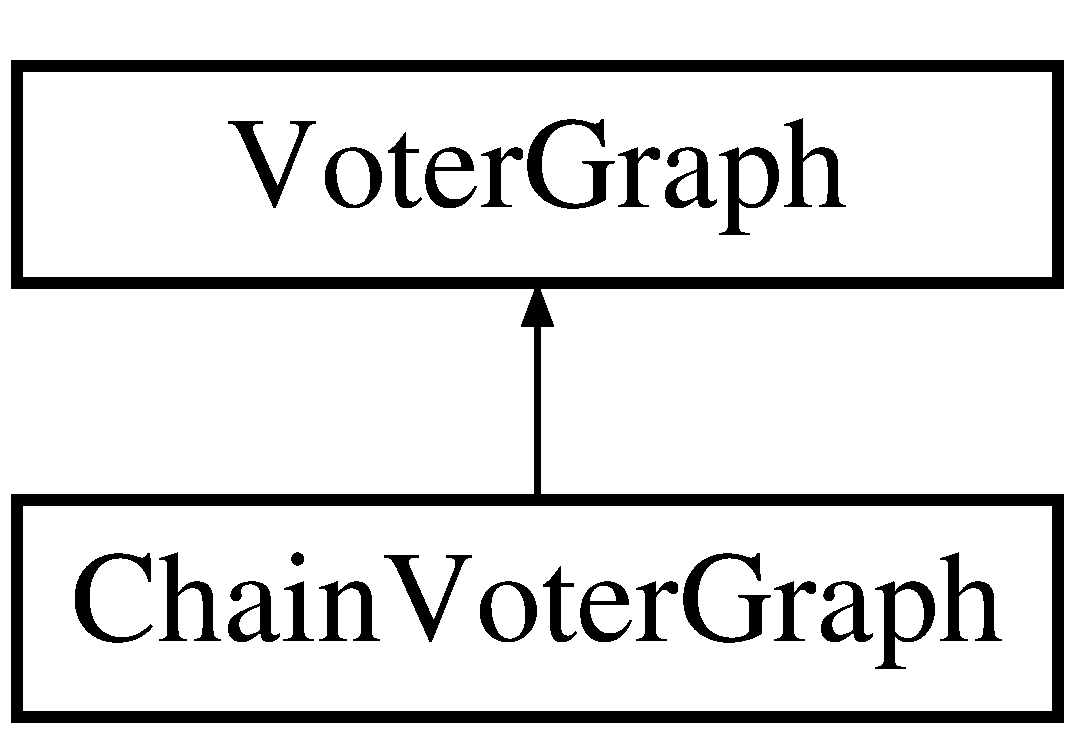
\includegraphics[height=2.000000cm]{class_chain_voter_graph}
\end{center}
\end{figure}
\subsection*{Public Member Functions}
\begin{DoxyCompactItemize}
\item 
\hypertarget{class_chain_voter_graph_af0e0e5327d26e67d46df0b33bb009c69}{{\bfseries Chain\-Voter\-Graph} (int size, double contrarian=0, bool ring=false, int update=\hyperlink{voter__graph_8hpp_ab3bec55c359e4ed771339c8bc61fc35aa01d100088352e1a7d3a34c9a66d0f951}{U\-P\-D\-A\-T\-E\-\_\-\-E\-D\-G\-E\-S})}\label{class_chain_voter_graph_af0e0e5327d26e67d46df0b33bb009c69}

\end{DoxyCompactItemize}
\subsection*{Public Attributes}
\begin{DoxyCompactItemize}
\item 
\hypertarget{class_chain_voter_graph_a03a3e2fb44bd8c4e0e1697545d4eff65}{int {\bfseries size}}\label{class_chain_voter_graph_a03a3e2fb44bd8c4e0e1697545d4eff65}

\item 
\hypertarget{class_chain_voter_graph_ace4b3a77876d38f216552e4b5bfaf32b}{double {\bfseries contrarian}}\label{class_chain_voter_graph_ace4b3a77876d38f216552e4b5bfaf32b}

\item 
\hypertarget{class_chain_voter_graph_a0b9e76e99e2666ca7e92ec757ce24d32}{\hyperlink{class_voter_node}{Voter\-Node} $\ast$$\ast$ {\bfseries node\-Array}}\label{class_chain_voter_graph_a0b9e76e99e2666ca7e92ec757ce24d32}

\item 
\hypertarget{class_chain_voter_graph_afb107128956fbedd499dfbfeef8fe14c}{bool {\bfseries ring}}\label{class_chain_voter_graph_afb107128956fbedd499dfbfeef8fe14c}

\end{DoxyCompactItemize}


The documentation for this class was generated from the following files\-:\begin{DoxyCompactItemize}
\item 
/home/lamarche/programming/multilevel\-\_\-prediction/src/\hyperlink{voter__graph_8hpp}{voter\-\_\-graph.\-hpp}\item 
/home/lamarche/programming/multilevel\-\_\-prediction/src/voter\-\_\-graph.\-cpp\end{DoxyCompactItemize}

\hypertarget{class_complete_voter_graph}{}\section{Complete\+Voter\+Graph Class Reference}
\label{class_complete_voter_graph}\index{Complete\+Voter\+Graph@{Complete\+Voter\+Graph}}


An interaction graph with edges between each pair of nodes (in both direction, with equal weight for each edge)  




{\ttfamily \#include $<$voter\+\_\+graph.\+hpp$>$}

Inheritance diagram for Complete\+Voter\+Graph\+:\begin{figure}[H]
\begin{center}
\leavevmode
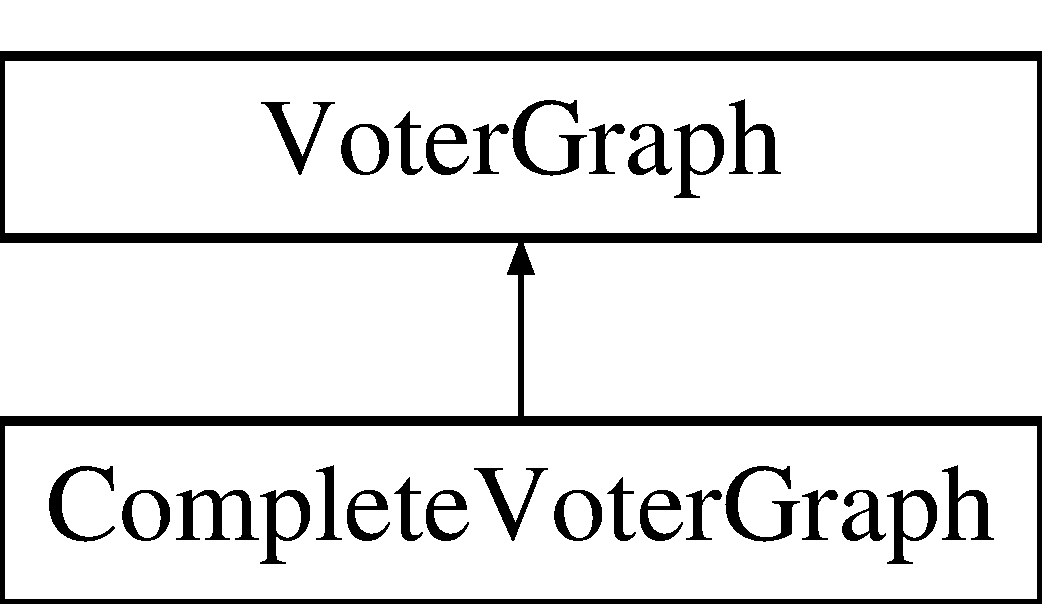
\includegraphics[height=2.000000cm]{class_complete_voter_graph}
\end{center}
\end{figure}
\subsection*{Public Member Functions}
\begin{DoxyCompactItemize}
\item 
\hyperlink{class_complete_voter_graph_a0adf42ee4826aa54e1a13d9b8d770554}{Complete\+Voter\+Graph} (int size, int update=\hyperlink{voter__graph_8hpp_a305d80651467e931f258a3686976d31c}{U\+P\+D\+A\+T\+E\+\_\+\+E\+D\+G\+E\+S}, double contrarian=0)
\begin{DoxyCompactList}\small\item\em Constructor. \end{DoxyCompactList}\end{DoxyCompactItemize}
\subsection*{Additional Inherited Members}


\subsection{Detailed Description}
An interaction graph with edges between each pair of nodes (in both direction, with equal weight for each edge) 

\subsection{Constructor \& Destructor Documentation}
\hypertarget{class_complete_voter_graph_a0adf42ee4826aa54e1a13d9b8d770554}{}\index{Complete\+Voter\+Graph@{Complete\+Voter\+Graph}!Complete\+Voter\+Graph@{Complete\+Voter\+Graph}}
\index{Complete\+Voter\+Graph@{Complete\+Voter\+Graph}!Complete\+Voter\+Graph@{Complete\+Voter\+Graph}}
\subsubsection[{Complete\+Voter\+Graph}]{\setlength{\rightskip}{0pt plus 5cm}Complete\+Voter\+Graph\+::\+Complete\+Voter\+Graph (
\begin{DoxyParamCaption}
\item[{int}]{size, }
\item[{int}]{update = {\ttfamily {\bf U\+P\+D\+A\+T\+E\+\_\+\+E\+D\+G\+E\+S}}, }
\item[{double}]{contrarian = {\ttfamily 0}}
\end{DoxyParamCaption}
)}\label{class_complete_voter_graph_a0adf42ee4826aa54e1a13d9b8d770554}


Constructor. 


\begin{DoxyParams}{Parameters}
{\em size} & \+: Size of the graph \\
\hline
{\em update} & \+: How the system evolves at each simulation step (U\+P\+D\+A\+T\+E\+\_\+\+N\+O\+D\+E\+S or U\+P\+D\+A\+T\+E\+\_\+\+E\+D\+G\+E\+S) \\
\hline
{\em contrarian} & \+: The contrarian rate of each node \\
\hline
\end{DoxyParams}


The documentation for this class was generated from the following files\+:\begin{DoxyCompactItemize}
\item 
C\+:/\+Users/\+Robin/\+Mes projets/programming/multilevel\+\_\+prediction/src/\hyperlink{voter__graph_8hpp}{voter\+\_\+graph.\+hpp}\item 
C\+:/\+Users/\+Robin/\+Mes projets/programming/multilevel\+\_\+prediction/src/voter\+\_\+graph.\+cpp\end{DoxyCompactItemize}

\hypertarget{struct_data_point_struct}{}\section{Data\+Point\+Struct Struct Reference}
\label{struct_data_point_struct}\index{Data\+Point\+Struct@{Data\+Point\+Struct}}
\subsection*{Public Attributes}
\begin{DoxyCompactItemize}
\item 
\hypertarget{struct_data_point_struct_ac42ecde939c4bb686fbe3ce67d5c34e3}{}int {\bfseries size}\label{struct_data_point_struct_ac42ecde939c4bb686fbe3ce67d5c34e3}

\item 
\hypertarget{struct_data_point_struct_ae1dae54ff363ef8a6d946907b1621506}{}float {\bfseries time}\label{struct_data_point_struct_ae1dae54ff363ef8a6d946907b1621506}

\item 
\hypertarget{struct_data_point_struct_a6d345b8aa7e79cd06402446d73d19520}{}int {\bfseries memory}\label{struct_data_point_struct_a6d345b8aa7e79cd06402446d73d19520}

\end{DoxyCompactItemize}


The documentation for this struct was generated from the following file\+:\begin{DoxyCompactItemize}
\item 
C\+:/\+Users/\+Robin/\+Mes projets/programming/multilevel\+\_\+prediction/src/timer.\+hpp\end{DoxyCompactItemize}

\hypertarget{class_empty_voter_measurement}{}\section{Empty\+Voter\+Measurement Class Reference}
\label{class_empty_voter_measurement}\index{Empty\+Voter\+Measurement@{Empty\+Voter\+Measurement}}


A measurement without any probe (no observation)  




{\ttfamily \#include $<$voter\+\_\+graph.\+hpp$>$}

Inheritance diagram for Empty\+Voter\+Measurement\+:\begin{figure}[H]
\begin{center}
\leavevmode
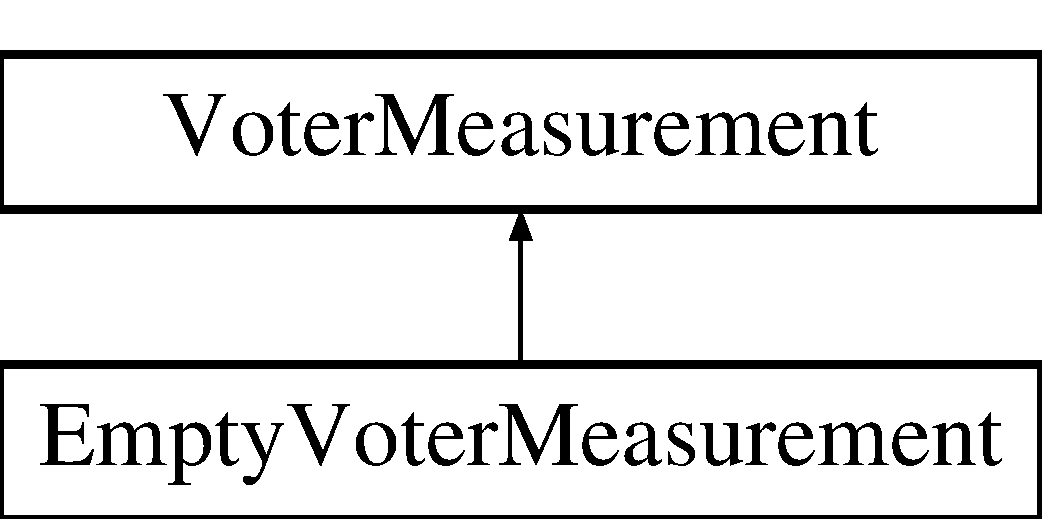
\includegraphics[height=2.000000cm]{class_empty_voter_measurement}
\end{center}
\end{figure}
\subsection*{Public Member Functions}
\begin{DoxyCompactItemize}
\item 
\hyperlink{class_empty_voter_measurement_aff7c264f9f2e68e3608e30b359468ed0}{Empty\+Voter\+Measurement} (\hyperlink{class_voter_graph}{Voter\+Graph} $\ast$\hyperlink{class_voter_measurement_a8d22d4b78f7e2f4c747f5716c4885351}{graph})
\begin{DoxyCompactList}\small\item\em Constructor. \end{DoxyCompactList}\end{DoxyCompactItemize}
\subsection*{Additional Inherited Members}


\subsection{Detailed Description}
A measurement without any probe (no observation) 

\subsection{Constructor \& Destructor Documentation}
\hypertarget{class_empty_voter_measurement_aff7c264f9f2e68e3608e30b359468ed0}{}\index{Empty\+Voter\+Measurement@{Empty\+Voter\+Measurement}!Empty\+Voter\+Measurement@{Empty\+Voter\+Measurement}}
\index{Empty\+Voter\+Measurement@{Empty\+Voter\+Measurement}!Empty\+Voter\+Measurement@{Empty\+Voter\+Measurement}}
\subsubsection[{Empty\+Voter\+Measurement}]{\setlength{\rightskip}{0pt plus 5cm}Empty\+Voter\+Measurement\+::\+Empty\+Voter\+Measurement (
\begin{DoxyParamCaption}
\item[{{\bf Voter\+Graph} $\ast$}]{graph}
\end{DoxyParamCaption}
)}\label{class_empty_voter_measurement_aff7c264f9f2e68e3608e30b359468ed0}


Constructor. 


\begin{DoxyParams}{Parameters}
{\em graph} & \+: The interaction graph to be observed \\
\hline
\end{DoxyParams}


The documentation for this class was generated from the following files\+:\begin{DoxyCompactItemize}
\item 
C\+:/\+Users/\+Robin/\+Mes projets/programming/multilevel\+\_\+prediction/src/\hyperlink{voter__graph_8hpp}{voter\+\_\+graph.\+hpp}\item 
C\+:/\+Users/\+Robin/\+Mes projets/programming/multilevel\+\_\+prediction/src/voter\+\_\+graph.\+cpp\end{DoxyCompactItemize}

\hypertarget{class_macro_voter_measurement}{\section{Macro\-Voter\-Measurement Class Reference}
\label{class_macro_voter_measurement}\index{Macro\-Voter\-Measurement@{Macro\-Voter\-Measurement}}
}


A measurement consisting in one probe observing all nodes of the interaction graph.  




{\ttfamily \#include $<$voter\-\_\-graph.\-hpp$>$}

Inheritance diagram for Macro\-Voter\-Measurement\-:\begin{figure}[H]
\begin{center}
\leavevmode
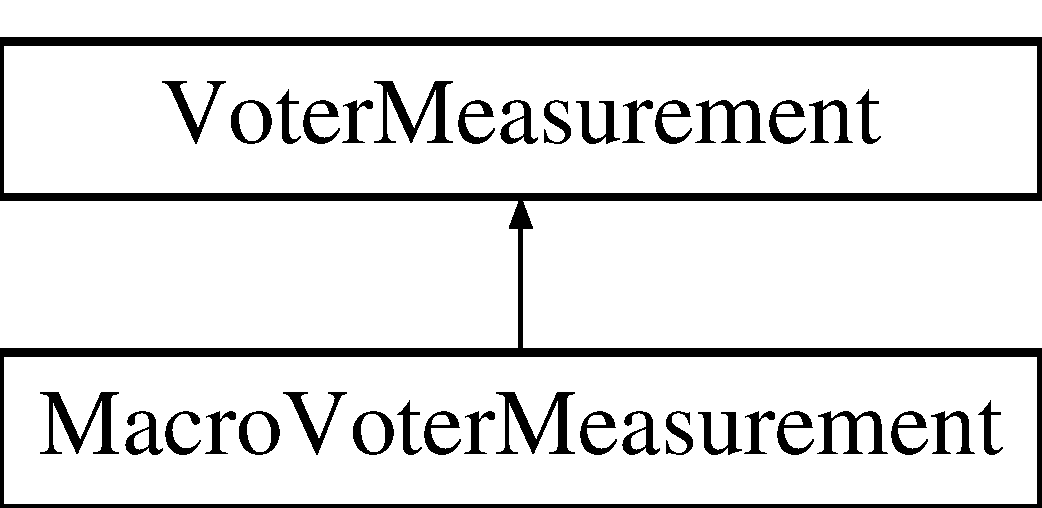
\includegraphics[height=2.000000cm]{class_macro_voter_measurement}
\end{center}
\end{figure}
\subsection*{Public Member Functions}
\begin{DoxyCompactItemize}
\item 
\hyperlink{class_macro_voter_measurement_a5198644e81ae6561fd8d53e3a944328d}{Macro\-Voter\-Measurement} (\hyperlink{class_voter_graph}{Voter\-Graph} $\ast$\hyperlink{class_voter_measurement_a8d22d4b78f7e2f4c747f5716c4885351}{graph}, std\-::set$<$ \hyperlink{voter__graph_8hpp_acb4c45a5ce4a55eee28e54e60409b9c5}{Voter\-Metric} $>$ metrics)
\begin{DoxyCompactList}\small\item\em Constructor. \end{DoxyCompactList}\end{DoxyCompactItemize}
\subsection*{Additional Inherited Members}


\subsection{Detailed Description}
A measurement consisting in one probe observing all nodes of the interaction graph. 

\subsection{Constructor \& Destructor Documentation}
\hypertarget{class_macro_voter_measurement_a5198644e81ae6561fd8d53e3a944328d}{\index{Macro\-Voter\-Measurement@{Macro\-Voter\-Measurement}!Macro\-Voter\-Measurement@{Macro\-Voter\-Measurement}}
\index{Macro\-Voter\-Measurement@{Macro\-Voter\-Measurement}!MacroVoterMeasurement@{Macro\-Voter\-Measurement}}
\subsubsection[{Macro\-Voter\-Measurement}]{\setlength{\rightskip}{0pt plus 5cm}Macro\-Voter\-Measurement\-::\-Macro\-Voter\-Measurement (
\begin{DoxyParamCaption}
\item[{{\bf Voter\-Graph} $\ast$}]{graph, }
\item[{std\-::set$<$ {\bf Voter\-Metric} $>$}]{metrics}
\end{DoxyParamCaption}
)}}\label{class_macro_voter_measurement_a5198644e81ae6561fd8d53e3a944328d}


Constructor. 


\begin{DoxyParams}{Parameters}
{\em graph} & \-: The interaction graph to be observed \\
\hline
{\em metrics} & \-: The set of metrics associated to the macro-\/probe \\
\hline
\end{DoxyParams}


The documentation for this class was generated from the following files\-:\begin{DoxyCompactItemize}
\item 
/home/lamarche/programming/multilevel\-\_\-prediction/src/\hyperlink{voter__graph_8hpp}{voter\-\_\-graph.\-hpp}\item 
/home/lamarche/programming/multilevel\-\_\-prediction/src/voter\-\_\-graph.\-cpp\end{DoxyCompactItemize}

\hypertarget{class_markov_data_set}{\section{Markov\-Data\-Set Class Reference}
\label{class_markov_data_set}\index{Markov\-Data\-Set@{Markov\-Data\-Set}}
}
\subsection*{Public Member Functions}
\begin{DoxyCompactItemize}
\item 
\hypertarget{class_markov_data_set_af5652def3bd861e32423628515212e1a}{{\bfseries Markov\-Data\-Set} (\hyperlink{class_markov_process}{Markov\-Process} $\ast$process, int size, int time, int length)}\label{class_markov_data_set_af5652def3bd861e32423628515212e1a}

\item 
\hypertarget{class_markov_data_set_a90e28188b58acc59d75d44e01022e180}{double {\bfseries compute\-Score} (\hyperlink{class_partition}{Partition} $\ast$pre\-P, \hyperlink{class_partition}{Partition} $\ast$post\-P, int delay, int training\-Length)}\label{class_markov_data_set_a90e28188b58acc59d75d44e01022e180}

\end{DoxyCompactItemize}
\subsection*{Public Attributes}
\begin{DoxyCompactItemize}
\item 
\hypertarget{class_markov_data_set_a4634e9ebbab3500e07fc039b7917c219}{\hyperlink{class_markov_process}{Markov\-Process} $\ast$ {\bfseries process}}\label{class_markov_data_set_a4634e9ebbab3500e07fc039b7917c219}

\item 
\hypertarget{class_markov_data_set_ad00c1b3025f6fcbd67e7c23b456962bd}{int {\bfseries size}}\label{class_markov_data_set_ad00c1b3025f6fcbd67e7c23b456962bd}

\item 
\hypertarget{class_markov_data_set_a5ac0cfb2d1cbe80c7f4e6c980c93dcdd}{int {\bfseries time}}\label{class_markov_data_set_a5ac0cfb2d1cbe80c7f4e6c980c93dcdd}

\item 
\hypertarget{class_markov_data_set_a4506dddc00f33e4e889a5de277bd2966}{int {\bfseries length}}\label{class_markov_data_set_a4506dddc00f33e4e889a5de277bd2966}

\item 
\hypertarget{class_markov_data_set_aee1a6c899637e2c9cc3c22977b17f7b2}{\hyperlink{class_markov_trajectory}{Markov\-Trajectory} $\ast$$\ast$ {\bfseries trajectories}}\label{class_markov_data_set_aee1a6c899637e2c9cc3c22977b17f7b2}

\end{DoxyCompactItemize}


The documentation for this class was generated from the following files\-:\begin{DoxyCompactItemize}
\item 
/home/lamarche/programming/multilevel\-\_\-prediction/src/\hyperlink{markov__process_8hpp}{markov\-\_\-process.\-hpp}\item 
/home/lamarche/programming/multilevel\-\_\-prediction/src/markov\-\_\-process.\-cpp\end{DoxyCompactItemize}

\hypertarget{class_markov_process}{}\section{Markov\+Process Class Reference}
\label{class_markov_process}\index{Markov\+Process@{Markov\+Process}}
\subsection*{Public Member Functions}
\begin{DoxyCompactItemize}
\item 
\hypertarget{class_markov_process_a6dbcf0cf4a855b803c57d3e69bb42a7d}{}{\bfseries Markov\+Process} (int size)\label{class_markov_process_a6dbcf0cf4a855b803c57d3e69bb42a7d}

\item 
\hypertarget{class_markov_process_acee38f7c8f384f9be422c965a0efc4fb}{}void {\bfseries print} ()\label{class_markov_process_acee38f7c8f384f9be422c965a0efc4fb}

\item 
\hypertarget{class_markov_process_a2942db4262f73c20cc49bfebaf0df101}{}void {\bfseries set\+Distribution} (double $\ast$array)\label{class_markov_process_a2942db4262f73c20cc49bfebaf0df101}

\item 
\hypertarget{class_markov_process_a1dfca569e38a94214afc152c5b0c2567}{}void {\bfseries set\+Transition} (int j, double $\ast$array)\label{class_markov_process_a1dfca569e38a94214afc152c5b0c2567}

\item 
\hypertarget{class_markov_process_a687c9c983ac090f2ba40d028c6f04786}{}void {\bfseries set\+Transition} (double $\ast$array)\label{class_markov_process_a687c9c983ac090f2ba40d028c6f04786}

\item 
\hypertarget{class_markov_process_afa7edaa775112df8dd4fc5007034d7e7}{}double $\ast$ {\bfseries get\+Distribution} (int time)\label{class_markov_process_afa7edaa775112df8dd4fc5007034d7e7}

\item 
\hypertarget{class_markov_process_a39c87840da9b238d7c33bd5ad23d538d}{}double $\ast$ {\bfseries get\+Transition} (int delay)\label{class_markov_process_a39c87840da9b238d7c33bd5ad23d538d}

\item 
\hypertarget{class_markov_process_a77be24a3ccec6e19ba922f932d19e0fa}{}void {\bfseries compute\+Stationary\+Distribution} (double threshold)\label{class_markov_process_a77be24a3ccec6e19ba922f932d19e0fa}

\item 
\hypertarget{class_markov_process_a6cd7abb0de322eb2ee133eda283388c3}{}double $\ast$ {\bfseries get\+Stationary\+Distribution} ()\label{class_markov_process_a6cd7abb0de322eb2ee133eda283388c3}

\item 
\hypertarget{class_markov_process_a4ed608f200c71a15ae4140b0f1305a88}{}double {\bfseries get\+Probability} (int individuals, int current\+Time)\label{class_markov_process_a4ed608f200c71a15ae4140b0f1305a88}

\item 
\hypertarget{class_markov_process_afe80afb9c456631a9168c762058d3cd2}{}double {\bfseries get\+Probability} (\hyperlink{class_part}{Part} $\ast$part, int current\+Time)\label{class_markov_process_afe80afb9c456631a9168c762058d3cd2}

\item 
\hypertarget{class_markov_process_ab17f4ae9fa56c009553a5d50e899a84b}{}double {\bfseries get\+Next\+Probability} (int next\+Individual, int current\+Individual, int delay)\label{class_markov_process_ab17f4ae9fa56c009553a5d50e899a84b}

\item 
\hypertarget{class_markov_process_a254635ef2e405073dd19aa14aa4ec365}{}double {\bfseries get\+Next\+Probability} (\hyperlink{class_part}{Part} $\ast$next\+Part, int current\+Individual, int delay)\label{class_markov_process_a254635ef2e405073dd19aa14aa4ec365}

\item 
\hypertarget{class_markov_process_a72033d86b846a06449a005f796ec14c1}{}double {\bfseries get\+Next\+Probability} (\hyperlink{class_part}{Part} $\ast$next\+Part, \hyperlink{class_part}{Part} $\ast$current\+Part, int delay, int time)\label{class_markov_process_a72033d86b846a06449a005f796ec14c1}

\item 
\hypertarget{class_markov_process_ad1d295d33c8abc5bdabea3eeaf33b553}{}double {\bfseries get\+Entropy} (\hyperlink{class_partition}{Partition} $\ast$partition, int current\+Time)\label{class_markov_process_ad1d295d33c8abc5bdabea3eeaf33b553}

\item 
\hypertarget{class_markov_process_a37aa6fee427f28a0d44dc369a2fd3b6a}{}double {\bfseries get\+Mutual\+Information} (\hyperlink{class_partition}{Partition} $\ast$next\+Partition, \hyperlink{class_partition}{Partition} $\ast$current\+Partition, int delay, int time)\label{class_markov_process_a37aa6fee427f28a0d44dc369a2fd3b6a}

\item 
\hypertarget{class_markov_process_a85b3be2d849c1b21ad1f98f06816ed76}{}double {\bfseries get\+Next\+Entropy} (\hyperlink{class_partition}{Partition} $\ast$partition, bool micro, int time)\label{class_markov_process_a85b3be2d849c1b21ad1f98f06816ed76}

\item 
\hypertarget{class_markov_process_a619919d687122a85e49368a5cf545a86}{}double {\bfseries get\+Closure\+Measure} (\hyperlink{class_partition}{Partition} $\ast$partition, int time)\label{class_markov_process_a619919d687122a85e49368a5cf545a86}

\end{DoxyCompactItemize}
\subsection*{Public Attributes}
\begin{DoxyCompactItemize}
\item 
\hypertarget{class_markov_process_ad38170c3a73d113dc152e73bc57d0523}{}int {\bfseries size}\label{class_markov_process_ad38170c3a73d113dc152e73bc57d0523}

\item 
\hypertarget{class_markov_process_ab08fd1641b1f866be6a7e3dcca7ed575}{}double $\ast$ {\bfseries distribution}\label{class_markov_process_ab08fd1641b1f866be6a7e3dcca7ed575}

\item 
\hypertarget{class_markov_process_a8e5ced320dd6b0a41c2f38f316c37cbf}{}std\+::vector$<$ double $\ast$ $>$ $\ast$ {\bfseries distributions}\label{class_markov_process_a8e5ced320dd6b0a41c2f38f316c37cbf}

\item 
\hypertarget{class_markov_process_a5eddf681cb7bc196a248813ba42b516f}{}int {\bfseries last\+Time}\label{class_markov_process_a5eddf681cb7bc196a248813ba42b516f}

\item 
\hypertarget{class_markov_process_aae914f9e4fa973b5515bebc41508a289}{}double $\ast$ {\bfseries transition}\label{class_markov_process_aae914f9e4fa973b5515bebc41508a289}

\item 
\hypertarget{class_markov_process_a16e4250dba911530aff3d2766a367e5b}{}std\+::vector$<$ double $\ast$ $>$ $\ast$ {\bfseries transitions}\label{class_markov_process_a16e4250dba911530aff3d2766a367e5b}

\item 
\hypertarget{class_markov_process_a5fa10a819200afd87b558332b6e351a6}{}int {\bfseries last\+Delay}\label{class_markov_process_a5fa10a819200afd87b558332b6e351a6}

\end{DoxyCompactItemize}


The documentation for this class was generated from the following files\+:\begin{DoxyCompactItemize}
\item 
C\+:/\+Users/\+Robin/\+Mes projets/programming/multilevel\+\_\+prediction/src/markov\+\_\+process.\+hpp\item 
C\+:/\+Users/\+Robin/\+Mes projets/programming/multilevel\+\_\+prediction/src/markov\+\_\+process.\+cpp\end{DoxyCompactItemize}

\hypertarget{class_markov_trajectory}{\section{Markov\-Trajectory Class Reference}
\label{class_markov_trajectory}\index{Markov\-Trajectory@{Markov\-Trajectory}}
}
\subsection*{Public Member Functions}
\begin{DoxyCompactItemize}
\item 
\hypertarget{class_markov_trajectory_a87acf0aef9d85e369378d004e06c56de}{{\bfseries Markov\-Trajectory} (\hyperlink{class_markov_process}{Markov\-Process} $\ast$process, int time, int length)}\label{class_markov_trajectory_a87acf0aef9d85e369378d004e06c56de}

\item 
\hypertarget{class_markov_trajectory_a29bb2d19771e93e6c87204c8ac2b3bd1}{void {\bfseries print} (int binary=0)}\label{class_markov_trajectory_a29bb2d19771e93e6c87204c8ac2b3bd1}

\end{DoxyCompactItemize}
\subsection*{Public Attributes}
\begin{DoxyCompactItemize}
\item 
\hypertarget{class_markov_trajectory_ada9138be4456a51a6f86c491079b0a58}{\hyperlink{class_markov_process}{Markov\-Process} $\ast$ {\bfseries process}}\label{class_markov_trajectory_ada9138be4456a51a6f86c491079b0a58}

\item 
\hypertarget{class_markov_trajectory_ab9a7f6133864c100caee694f7fb5c272}{int {\bfseries time}}\label{class_markov_trajectory_ab9a7f6133864c100caee694f7fb5c272}

\item 
\hypertarget{class_markov_trajectory_a12f640932269482c40e2a8efb9ff61c1}{int {\bfseries length}}\label{class_markov_trajectory_a12f640932269482c40e2a8efb9ff61c1}

\item 
\hypertarget{class_markov_trajectory_af7aa190f73505e8eb514ca7725572268}{int $\ast$ {\bfseries states}}\label{class_markov_trajectory_af7aa190f73505e8eb514ca7725572268}

\end{DoxyCompactItemize}


The documentation for this class was generated from the following files\-:\begin{DoxyCompactItemize}
\item 
/home/lamarche/programming/multilevel\-\_\-prediction/src/\hyperlink{markov__process_8hpp}{markov\-\_\-process.\-hpp}\item 
/home/lamarche/programming/multilevel\-\_\-prediction/src/markov\-\_\-process.\-cpp\end{DoxyCompactItemize}

\hypertarget{class_micro_voter_measurement}{\section{Micro\-Voter\-Measurement Class Reference}
\label{class_micro_voter_measurement}\index{Micro\-Voter\-Measurement@{Micro\-Voter\-Measurement}}
}


A measurement consisting in one probe for each node of the interaction graph.  




{\ttfamily \#include $<$voter\-\_\-graph.\-hpp$>$}

Inheritance diagram for Micro\-Voter\-Measurement\-:\begin{figure}[H]
\begin{center}
\leavevmode
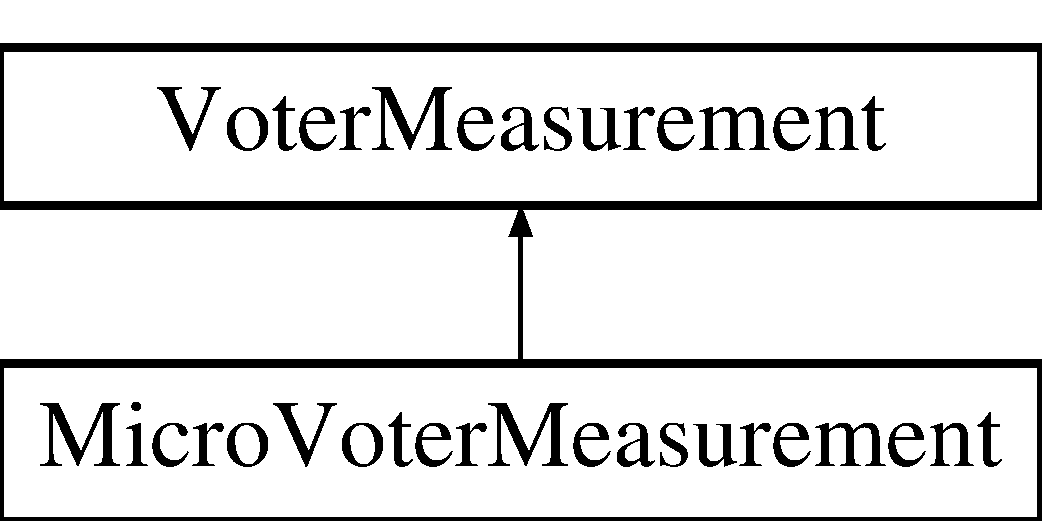
\includegraphics[height=2.000000cm]{class_micro_voter_measurement}
\end{center}
\end{figure}
\subsection*{Public Member Functions}
\begin{DoxyCompactItemize}
\item 
\hyperlink{class_micro_voter_measurement_a5ab772e26666d7ddf100a0cfea95afee}{Micro\-Voter\-Measurement} (\hyperlink{class_voter_graph}{Voter\-Graph} $\ast$\hyperlink{class_voter_measurement_a8d22d4b78f7e2f4c747f5716c4885351}{graph}, std\-::set$<$ \hyperlink{voter__graph_8hpp_acb4c45a5ce4a55eee28e54e60409b9c5}{Voter\-Metric} $>$ metric)
\begin{DoxyCompactList}\small\item\em Constructor. \end{DoxyCompactList}\end{DoxyCompactItemize}
\subsection*{Additional Inherited Members}


\subsection{Detailed Description}
A measurement consisting in one probe for each node of the interaction graph. 

\subsection{Constructor \& Destructor Documentation}
\hypertarget{class_micro_voter_measurement_a5ab772e26666d7ddf100a0cfea95afee}{\index{Micro\-Voter\-Measurement@{Micro\-Voter\-Measurement}!Micro\-Voter\-Measurement@{Micro\-Voter\-Measurement}}
\index{Micro\-Voter\-Measurement@{Micro\-Voter\-Measurement}!MicroVoterMeasurement@{Micro\-Voter\-Measurement}}
\subsubsection[{Micro\-Voter\-Measurement}]{\setlength{\rightskip}{0pt plus 5cm}Micro\-Voter\-Measurement\-::\-Micro\-Voter\-Measurement (
\begin{DoxyParamCaption}
\item[{{\bf Voter\-Graph} $\ast$}]{graph, }
\item[{std\-::set$<$ {\bf Voter\-Metric} $>$}]{metric}
\end{DoxyParamCaption}
)}}\label{class_micro_voter_measurement_a5ab772e26666d7ddf100a0cfea95afee}


Constructor. 


\begin{DoxyParams}{Parameters}
{\em graph} & \-: The interaction graph to be observed \\
\hline
{\em metric} & \-: The set of metric associated to the micro-\/probe \\
\hline
\end{DoxyParams}


The documentation for this class was generated from the following files\-:\begin{DoxyCompactItemize}
\item 
/home/lamarche/programming/multilevel\-\_\-prediction/src/\hyperlink{voter__graph_8hpp}{voter\-\_\-graph.\-hpp}\item 
/home/lamarche/programming/multilevel\-\_\-prediction/src/voter\-\_\-graph.\-cpp\end{DoxyCompactItemize}

\hypertarget{class_ordered_partition}{\section{Ordered\-Partition Class Reference}
\label{class_ordered_partition}\index{Ordered\-Partition@{Ordered\-Partition}}
}
\subsection*{Public Member Functions}
\begin{DoxyCompactItemize}
\item 
\hypertarget{class_ordered_partition_aabf4e3ee7ddd8279efd1d30f13844dbf}{{\bfseries Ordered\-Partition} (int s, double p)}\label{class_ordered_partition_aabf4e3ee7ddd8279efd1d30f13844dbf}

\item 
\hypertarget{class_ordered_partition_ad62349b410a52274043a328dafb13342}{void {\bfseries print} ()}\label{class_ordered_partition_ad62349b410a52274043a328dafb13342}

\end{DoxyCompactItemize}
\subsection*{Public Attributes}
\begin{DoxyCompactItemize}
\item 
\hypertarget{class_ordered_partition_ac4e60b2ef3d286b496d3274f153ff610}{int {\bfseries micro\-Size}}\label{class_ordered_partition_ac4e60b2ef3d286b496d3274f153ff610}

\item 
\hypertarget{class_ordered_partition_aa87bf05471b9071a94cf53226552f436}{int $\ast$ {\bfseries optimal\-Cut}}\label{class_ordered_partition_aa87bf05471b9071a94cf53226552f436}

\item 
\hypertarget{class_ordered_partition_a8c7fef058b25165c69652e8c78d9bd7e}{double {\bfseries param}}\label{class_ordered_partition_a8c7fef058b25165c69652e8c78d9bd7e}

\item 
\hypertarget{class_ordered_partition_a68c0b17fa5a9fc525af12b9960874ae7}{double {\bfseries beta}}\label{class_ordered_partition_a68c0b17fa5a9fc525af12b9960874ae7}

\item 
\hypertarget{class_ordered_partition_a6508f965f7e829e361c5d73acccce6eb}{std\-::string {\bfseries string}}\label{class_ordered_partition_a6508f965f7e829e361c5d73acccce6eb}

\item 
\hypertarget{class_ordered_partition_acc541302636a852fbb51c876277595a9}{double {\bfseries entropy}}\label{class_ordered_partition_acc541302636a852fbb51c876277595a9}

\item 
\hypertarget{class_ordered_partition_a414f6978e006ba9d647e48ceef9143b8}{double {\bfseries information}}\label{class_ordered_partition_a414f6978e006ba9d647e48ceef9143b8}

\end{DoxyCompactItemize}


The documentation for this class was generated from the following file\-:\begin{DoxyCompactItemize}
\item 
/home/lamarche/programming/multilevel\-\_\-prediction/src/\hyperlink{partition_8hpp}{partition.\-hpp}\end{DoxyCompactItemize}

\hypertarget{class_part}{}\section{Part Class Reference}
\label{class_part}\index{Part@{Part}}
\subsection*{Public Member Functions}
\begin{DoxyCompactItemize}
\item 
\hypertarget{class_part_a4fc5eedff4d310041e3ebee54693f4ac}{}{\bfseries Part} (\hyperlink{class_part}{Part} $\ast$part)\label{class_part_a4fc5eedff4d310041e3ebee54693f4ac}

\item 
\hypertarget{class_part_aa711a575b6b5bb0080b4e9fa7e20bbe1}{}void {\bfseries add\+Individual} (int i, bool front=false)\label{class_part_aa711a575b6b5bb0080b4e9fa7e20bbe1}

\item 
\hypertarget{class_part_a8b37a2433f60fba0c5dcce393e4f5a86}{}virtual bool {\bfseries equal} (\hyperlink{class_part}{Part} $\ast$p)\label{class_part_a8b37a2433f60fba0c5dcce393e4f5a86}

\item 
\hypertarget{class_part_a2d3c13012c781d8651b820e60d57c724}{}virtual void {\bfseries print} (bool endl=false)\label{class_part_a2d3c13012c781d8651b820e60d57c724}

\item 
\hypertarget{class_part_a501f9fdbc4efd9ce00e1eef4a07f033e}{}virtual int {\bfseries print\+Size} ()\label{class_part_a501f9fdbc4efd9ce00e1eef4a07f033e}

\end{DoxyCompactItemize}
\subsection*{Public Attributes}
\begin{DoxyCompactItemize}
\item 
\hypertarget{class_part_a12f364b91efb5702af492cbdef1990fe}{}std\+::list$<$ int $>$ $\ast$ {\bfseries individuals}\label{class_part_a12f364b91efb5702af492cbdef1990fe}

\end{DoxyCompactItemize}


The documentation for this class was generated from the following files\+:\begin{DoxyCompactItemize}
\item 
C\+:/\+Users/\+Robin/\+Mes projets/programming/multilevel\+\_\+prediction/src/partition.\+hpp\item 
C\+:/\+Users/\+Robin/\+Mes projets/programming/multilevel\+\_\+prediction/src/partition.\+cpp\end{DoxyCompactItemize}

\hypertarget{class_partition}{\section{Partition Class Reference}
\label{class_partition}\index{Partition@{Partition}}
}


A partition (i.\-e., a set of disjoint and covering parts)  




{\ttfamily \#include $<$partition.\-hpp$>$}

\subsection*{Public Member Functions}
\begin{DoxyCompactItemize}
\item 
\hypertarget{class_partition_acb291b3b0ccf48005e141be32fdd7efd}{{\bfseries Partition} (\hyperlink{class_partition}{Partition} $\ast$partition)}\label{class_partition_acb291b3b0ccf48005e141be32fdd7efd}

\item 
\hypertarget{class_partition_a63f82a3a75dc0c3d0d27766b2459c9fe}{void {\bfseries add\-Part} (\hyperlink{class_part}{Part} $\ast$p, bool front=false)}\label{class_partition_a63f82a3a75dc0c3d0d27766b2459c9fe}

\item 
\hypertarget{class_partition_ae21fdef95c1f37a6a677ac145f29b119}{\hyperlink{class_part}{Part} $\ast$ {\bfseries find\-Part} (int individual)}\label{class_partition_ae21fdef95c1f37a6a677ac145f29b119}

\item 
\hypertarget{class_partition_a76ac69e01cafef5af0fef2e917e6fdf1}{\hyperlink{class_part}{Part} $\ast$ {\bfseries get\-Part\-From\-Value} (int value)}\label{class_partition_a76ac69e01cafef5af0fef2e917e6fdf1}

\item 
\hypertarget{class_partition_abced08b339e293866a614b2f21414375}{bool {\bfseries equal} (\hyperlink{class_partition}{Partition} $\ast$p)}\label{class_partition_abced08b339e293866a614b2f21414375}

\item 
\hypertarget{class_partition_a3463b34ab90d020ed40635c473301a64}{void {\bfseries print} (bool endl=false)}\label{class_partition_a3463b34ab90d020ed40635c473301a64}

\end{DoxyCompactItemize}
\subsection*{Public Attributes}
\begin{DoxyCompactItemize}
\item 
\hypertarget{class_partition_a718bdba639f222d90d23480b58caa1f9}{int {\bfseries size}}\label{class_partition_a718bdba639f222d90d23480b58caa1f9}

\item 
\hypertarget{class_partition_a887cae6498c54754779d7956b48e8d3e}{std\-::list$<$ \hyperlink{class_part}{Part} $\ast$ $>$ $\ast$ {\bfseries parts}}\label{class_partition_a887cae6498c54754779d7956b48e8d3e}

\end{DoxyCompactItemize}


\subsection{Detailed Description}
A partition (i.\-e., a set of disjoint and covering parts) 

The documentation for this class was generated from the following files\-:\begin{DoxyCompactItemize}
\item 
/home/lamarche/programming/multilevel\-\_\-prediction/src/\hyperlink{partition_8hpp}{partition.\-hpp}\item 
/home/lamarche/programming/multilevel\-\_\-prediction/src/partition.\-cpp\end{DoxyCompactItemize}

\hypertarget{class_timer}{}\section{Timer Class Reference}
\label{class_timer}\index{Timer@{Timer}}
\subsection*{Public Member Functions}
\begin{DoxyCompactItemize}
\item 
\hypertarget{class_timer_a14edf0bdfc5a214895d321e7ae69365b}{}{\bfseries Timer} (char $\ast$file=0)\label{class_timer_a14edf0bdfc5a214895d321e7ae69365b}

\item 
\hypertarget{class_timer_acc61f0c4f2c1e26ba0bb62d367f0977e}{}void {\bfseries start} (int size, std\+::string text=\char`\"{}\char`\"{})\label{class_timer_acc61f0c4f2c1e26ba0bb62d367f0977e}

\item 
\hypertarget{class_timer_a5771baafd265be353ab78a4bb77329f9}{}void {\bfseries start\+Time} ()\label{class_timer_a5771baafd265be353ab78a4bb77329f9}

\item 
\hypertarget{class_timer_afada34fd58fb4729b9a6ee7a445f5133}{}void {\bfseries start\+Memory} ()\label{class_timer_afada34fd58fb4729b9a6ee7a445f5133}

\item 
\hypertarget{class_timer_afc259e85201ab94f291b36ed97dbd5e2}{}void {\bfseries stop} (std\+::string text=\char`\"{}\char`\"{})\label{class_timer_afc259e85201ab94f291b36ed97dbd5e2}

\item 
\hypertarget{class_timer_a71c4bba47ccad8ed4131922d1cd6d689}{}void {\bfseries stop\+Time} ()\label{class_timer_a71c4bba47ccad8ed4131922d1cd6d689}

\item 
\hypertarget{class_timer_a55ad7a96c2e75c4a1a7209c8eb89ee9d}{}void {\bfseries stop\+Memory} ()\label{class_timer_a55ad7a96c2e75c4a1a7209c8eb89ee9d}

\item 
\hypertarget{class_timer_a88fa29d9f2422df0ad2ed43b1c28cc04}{}void {\bfseries step} (std\+::string text=\char`\"{}\char`\"{})\label{class_timer_a88fa29d9f2422df0ad2ed43b1c28cc04}

\item 
\hypertarget{class_timer_af29968e93e56c8bf1de7c9f559dfae23}{}void {\bfseries print} (char $\ast$f\+Name)\label{class_timer_af29968e93e56c8bf1de7c9f559dfae23}

\end{DoxyCompactItemize}


The documentation for this class was generated from the following files\+:\begin{DoxyCompactItemize}
\item 
C\+:/\+Users/\+Robin/\+Mes projets/programming/multilevel\+\_\+prediction/src/timer.\+hpp\item 
C\+:/\+Users/\+Robin/\+Mes projets/programming/multilevel\+\_\+prediction/src/timer.\+cpp\end{DoxyCompactItemize}

\hypertarget{class_two_communities_experiment}{\section{Two\-Communities\-Experiment Class Reference}
\label{class_two_communities_experiment}\index{Two\-Communities\-Experiment@{Two\-Communities\-Experiment}}
}


Programming a prediction experiment on a two-\/communities Voter Model.  




{\ttfamily \#include $<$voter\-\_\-experiment.\-hpp$>$}

\subsection*{Public Member Functions}
\begin{DoxyCompactItemize}
\item 
\hyperlink{class_two_communities_experiment_a9f4318b842f0ca4c297e78edd480efde}{Two\-Communities\-Experiment} (int size1, int size2, double intra\-R1, double intra\-R2, double inter\-R1, double inter\-R2, double contrarian1, double contrarian2, double time, double delay, Spec\-Measurement\-Set $\ast$\hyperlink{class_two_communities_experiment_a1e681dca94bf8bf967d0586acee25ac1}{pre\-Measurements}, Spec\-Measurement\-Set $\ast$\hyperlink{class_two_communities_experiment_a78016b6845b3752c0a83f09793653ecc}{post\-Measurements})
\begin{DoxyCompactList}\small\item\em Constructor. \end{DoxyCompactList}\item 
\hypertarget{class_two_communities_experiment_ad446d179a6caf0e8d53986c26f5b95d1}{\hyperlink{class_two_communities_experiment_ad446d179a6caf0e8d53986c26f5b95d1}{$\sim$\-Two\-Communities\-Experiment} ()}\label{class_two_communities_experiment_ad446d179a6caf0e8d53986c26f5b95d1}

\begin{DoxyCompactList}\small\item\em Destructor. \end{DoxyCompactList}\end{DoxyCompactItemize}
\subsection*{Public Attributes}
\begin{DoxyCompactItemize}
\item 
int \hyperlink{class_two_communities_experiment_a0249e614ce0ab3e019b334634d857d1c}{id}
\item 
\hyperlink{voter__graph_8hpp_ab3bec55c359e4ed771339c8bc61fc35a}{Update\-Process} \hyperlink{class_two_communities_experiment_ad72f8a79b28ad213d7d050c5acc0272f}{update}
\item 
double \hyperlink{class_two_communities_experiment_a31d5e198fae6cb9993a95f77b44b3bae}{threshold}
\item 
bool \hyperlink{class_two_communities_experiment_a4ed3dfc7aa3920dc9cf2eb3762e2c801}{compact\-Model}
\item 
\hypertarget{class_two_communities_experiment_a8367875982e8221231e7edd8de3ed866}{bool {\bfseries with\-Aggregation}}\label{class_two_communities_experiment_a8367875982e8221231e7edd8de3ed866}

\item 
\hypertarget{class_two_communities_experiment_a3e312c20de2388dd5ed22fd53c18f01d}{bool {\bfseries part\-Decomposition}}\label{class_two_communities_experiment_a3e312c20de2388dd5ed22fd53c18f01d}

\item 
int \hyperlink{class_two_communities_experiment_a32820f7a153564c07f9b2c60b1b0a802}{size1\-Min}
\item 
int \hyperlink{class_two_communities_experiment_af5352ec73c0b6090e51e3757fc553be7}{size1\-Max}
\item 
int \hyperlink{class_two_communities_experiment_a094cc2008529793f463ce298d76e8663}{size1\-Step}
\item 
int \hyperlink{class_two_communities_experiment_a0735678625778f49f3f05d18b5248a55}{size2\-Min}
\item 
int \hyperlink{class_two_communities_experiment_ad2ad665e665ba1c2e5ec6ece13190d1e}{size2\-Max}
\item 
int \hyperlink{class_two_communities_experiment_a71ef9b90f7bf40e0c8c008c397ccc14b}{size2\-Step}
\item 
bool \hyperlink{class_two_communities_experiment_a6c541a1436eb884e86c593c02035de85}{equal\-Size}
\item 
double \hyperlink{class_two_communities_experiment_a30d694b0b619d1a7e0e1d5f25076c6c4}{intra\-R1\-Min}
\item 
double \hyperlink{class_two_communities_experiment_adee272669c4b4e6c5e74a59efe2670f7}{intra\-R1\-Max}
\item 
double \hyperlink{class_two_communities_experiment_a8d1110034d1f89f1cc5fdfc4d3a09cf4}{intra\-R1\-Step}
\item 
double \hyperlink{class_two_communities_experiment_afa05e622cd2e95ef81649822f012ffad}{intra\-R2\-Min}
\item 
double \hyperlink{class_two_communities_experiment_aea1cdf3d8087ad33685ff7caf80b8bc1}{intra\-R2\-Max}
\item 
double \hyperlink{class_two_communities_experiment_ad958587e2411b3f9d87882fef453f3f6}{intra\-R2\-Step}
\item 
double \hyperlink{class_two_communities_experiment_aa8c411e9ac8be5c46cc32495917e9766}{inter\-R1\-Min}
\item 
double \hyperlink{class_two_communities_experiment_a1c0d181f60179b5457478a43e64638e0}{inter\-R1\-Max}
\item 
double \hyperlink{class_two_communities_experiment_ac0977ad7c4e0c87534b60caebc34e8f0}{inter\-R1\-Step}
\item 
double \hyperlink{class_two_communities_experiment_a2eeda95baf7cbc8acf89d66b460144f5}{inter\-R2\-Min}
\item 
double \hyperlink{class_two_communities_experiment_afc9e3538d0944d687ae23e6ad2e2a3fa}{inter\-R2\-Max}
\item 
double \hyperlink{class_two_communities_experiment_aadc1e8bde8ba99c123d6deb62ef0024d}{inter\-R2\-Step}
\item 
bool \hyperlink{class_two_communities_experiment_a99af0c5678c67201a249206710e53412}{equal\-Intra\-Rate}
\item 
bool \hyperlink{class_two_communities_experiment_a18e10411ee94d1695a3d365e49ab9976}{equal\-Inter\-Rate}
\item 
bool \hyperlink{class_two_communities_experiment_ade325f42fa637fae8e1c5496216c6bac}{opposite\-Inter\-Rate}
\item 
double \hyperlink{class_two_communities_experiment_ae135249e20a7ebd0483b3f02426a7772}{contrarian1\-Min}
\item 
double \hyperlink{class_two_communities_experiment_a4e41e8b55ad9be67dba9008f4caf9998}{contrarian1\-Max}
\item 
double \hyperlink{class_two_communities_experiment_a6b7cedae14a26185c3e98ff22e02761f}{contrarian1\-Step}
\item 
double \hyperlink{class_two_communities_experiment_a249455fc220b534837f794e6d4e3d520}{contrarian2\-Min}
\item 
double \hyperlink{class_two_communities_experiment_ab62dc7711b0acc972341bebfe14979f0}{contrarian2\-Max}
\item 
double \hyperlink{class_two_communities_experiment_a26d60430432743c9314ae2eb52a88627}{contrarian2\-Step}
\item 
bool \hyperlink{class_two_communities_experiment_a025e1c71fcd6c77612e4ef6005ddef4d}{equal\-Contrarian}
\item 
int \hyperlink{class_two_communities_experiment_a5c4868cca512ddd93f7cbdac070a1ed8}{time\-Min}
\item 
int \hyperlink{class_two_communities_experiment_ad08bd64c47132b4dfa2ed6d3408bcc06}{time\-Max}
\item 
int \hyperlink{class_two_communities_experiment_a06a819e995ff4f8593202ef6a425175b}{time\-Step}
\item 
int \hyperlink{class_two_communities_experiment_a861de92ba064381cf31010a57470a4b2}{delay\-Min}
\item 
int \hyperlink{class_two_communities_experiment_ab71b1171faa83b900ea3fdac52e4e74c}{delay\-Max}
\item 
int \hyperlink{class_two_communities_experiment_a4f91ecade73ca085cfba2015e38b6b33}{delay\-Step}
\item 
Spec\-Measurement\-Set $\ast$ \hyperlink{class_two_communities_experiment_a1e681dca94bf8bf967d0586acee25ac1}{pre\-Measurements}
\item 
Spec\-Measurement\-Set $\ast$ \hyperlink{class_two_communities_experiment_a78016b6845b3752c0a83f09793653ecc}{post\-Measurements}
\end{DoxyCompactItemize}
\subsection*{Static Public Attributes}
\begin{DoxyCompactItemize}
\item 
static int \hyperlink{class_two_communities_experiment_ad4b14e0987399445740ff5a57fa4aa29}{id\-\_\-number} = 0
\end{DoxyCompactItemize}


\subsection{Detailed Description}
Programming a prediction experiment on a two-\/communities Voter Model. 

\subsection{Constructor \& Destructor Documentation}
\hypertarget{class_two_communities_experiment_a9f4318b842f0ca4c297e78edd480efde}{\index{Two\-Communities\-Experiment@{Two\-Communities\-Experiment}!Two\-Communities\-Experiment@{Two\-Communities\-Experiment}}
\index{Two\-Communities\-Experiment@{Two\-Communities\-Experiment}!TwoCommunitiesExperiment@{Two\-Communities\-Experiment}}
\subsubsection[{Two\-Communities\-Experiment}]{\setlength{\rightskip}{0pt plus 5cm}Two\-Communities\-Experiment\-::\-Two\-Communities\-Experiment (
\begin{DoxyParamCaption}
\item[{int}]{size1, }
\item[{int}]{size2, }
\item[{double}]{intra\-R1, }
\item[{double}]{intra\-R2, }
\item[{double}]{inter\-R1, }
\item[{double}]{inter\-R2, }
\item[{double}]{contrarian1, }
\item[{double}]{contrarian2, }
\item[{double}]{time, }
\item[{double}]{delay, }
\item[{Spec\-Measurement\-Set $\ast$}]{pre\-Measurements, }
\item[{Spec\-Measurement\-Set $\ast$}]{post\-Measurements}
\end{DoxyParamCaption}
)}}\label{class_two_communities_experiment_a9f4318b842f0ca4c297e78edd480efde}


Constructor. 


\begin{DoxyParams}{Parameters}
{\em size1} & \-: The size of community 1 in all experiments \\
\hline
{\em size2} & \-: The size of community 2 in all experiments \\
\hline
{\em intra\-R1} & \-: The weight of edges within community 1 in all experiments \\
\hline
{\em intra\-R2} & \-: The weight of edges within community 2 in all experiments \\
\hline
{\em inter\-R1} & \-: The weight of edges from community 1 to community 2 in all experiments \\
\hline
{\em inter\-R2} & \-: The weight of edges from community 2 to community 1 in all experiments \\
\hline
{\em contrarian1} & \-: The contrarian rate of nodes within community 1 in all experiments \\
\hline
{\em contrarian2} & \-: The contrarian rate of nodes within community 2 in all experiments \\
\hline
{\em time} & \-: The time of pre-\/measurement (-\/1 for stationary distribution) in all experiments \\
\hline
{\em delay} & \-: The delay before post-\/measurement in all experiments \\
\hline
{\em pre\-Measurements} & \-: A set of pre-\/measurement for prediction \\
\hline
{\em post\-Measurements} & \-: A set of post-\/measurement to be predicted \\
\hline
\end{DoxyParams}


\subsection{Member Data Documentation}
\hypertarget{class_two_communities_experiment_a4ed3dfc7aa3920dc9cf2eb3762e2c801}{\index{Two\-Communities\-Experiment@{Two\-Communities\-Experiment}!compact\-Model@{compact\-Model}}
\index{compact\-Model@{compact\-Model}!TwoCommunitiesExperiment@{Two\-Communities\-Experiment}}
\subsubsection[{compact\-Model}]{\setlength{\rightskip}{0pt plus 5cm}bool Two\-Communities\-Experiment\-::compact\-Model}}\label{class_two_communities_experiment_a4ed3dfc7aa3920dc9cf2eb3762e2c801}
If true, the computed microscopic Markov chain is lumped according to the macro-\/state of community 1, the macro-\/state of community 2, and the state of the first agent in community 1 \hypertarget{class_two_communities_experiment_a4e41e8b55ad9be67dba9008f4caf9998}{\index{Two\-Communities\-Experiment@{Two\-Communities\-Experiment}!contrarian1\-Max@{contrarian1\-Max}}
\index{contrarian1\-Max@{contrarian1\-Max}!TwoCommunitiesExperiment@{Two\-Communities\-Experiment}}
\subsubsection[{contrarian1\-Max}]{\setlength{\rightskip}{0pt plus 5cm}double Two\-Communities\-Experiment\-::contrarian1\-Max}}\label{class_two_communities_experiment_a4e41e8b55ad9be67dba9008f4caf9998}
The contrarian rate of nodes within community 1 in the last experiment \hypertarget{class_two_communities_experiment_ae135249e20a7ebd0483b3f02426a7772}{\index{Two\-Communities\-Experiment@{Two\-Communities\-Experiment}!contrarian1\-Min@{contrarian1\-Min}}
\index{contrarian1\-Min@{contrarian1\-Min}!TwoCommunitiesExperiment@{Two\-Communities\-Experiment}}
\subsubsection[{contrarian1\-Min}]{\setlength{\rightskip}{0pt plus 5cm}double Two\-Communities\-Experiment\-::contrarian1\-Min}}\label{class_two_communities_experiment_ae135249e20a7ebd0483b3f02426a7772}
The contrarian rate of nodes within community 1 in the first experiment \hypertarget{class_two_communities_experiment_a6b7cedae14a26185c3e98ff22e02761f}{\index{Two\-Communities\-Experiment@{Two\-Communities\-Experiment}!contrarian1\-Step@{contrarian1\-Step}}
\index{contrarian1\-Step@{contrarian1\-Step}!TwoCommunitiesExperiment@{Two\-Communities\-Experiment}}
\subsubsection[{contrarian1\-Step}]{\setlength{\rightskip}{0pt plus 5cm}double Two\-Communities\-Experiment\-::contrarian1\-Step}}\label{class_two_communities_experiment_a6b7cedae14a26185c3e98ff22e02761f}
The contrarian rate of nodes within community 1 between two consecutive experiments \hypertarget{class_two_communities_experiment_ab62dc7711b0acc972341bebfe14979f0}{\index{Two\-Communities\-Experiment@{Two\-Communities\-Experiment}!contrarian2\-Max@{contrarian2\-Max}}
\index{contrarian2\-Max@{contrarian2\-Max}!TwoCommunitiesExperiment@{Two\-Communities\-Experiment}}
\subsubsection[{contrarian2\-Max}]{\setlength{\rightskip}{0pt plus 5cm}double Two\-Communities\-Experiment\-::contrarian2\-Max}}\label{class_two_communities_experiment_ab62dc7711b0acc972341bebfe14979f0}
The contrarian rate of nodes within community 2 in the last experiment \hypertarget{class_two_communities_experiment_a249455fc220b534837f794e6d4e3d520}{\index{Two\-Communities\-Experiment@{Two\-Communities\-Experiment}!contrarian2\-Min@{contrarian2\-Min}}
\index{contrarian2\-Min@{contrarian2\-Min}!TwoCommunitiesExperiment@{Two\-Communities\-Experiment}}
\subsubsection[{contrarian2\-Min}]{\setlength{\rightskip}{0pt plus 5cm}double Two\-Communities\-Experiment\-::contrarian2\-Min}}\label{class_two_communities_experiment_a249455fc220b534837f794e6d4e3d520}
The contrarian rate of nodes within community 2 in the first experiment \hypertarget{class_two_communities_experiment_a26d60430432743c9314ae2eb52a88627}{\index{Two\-Communities\-Experiment@{Two\-Communities\-Experiment}!contrarian2\-Step@{contrarian2\-Step}}
\index{contrarian2\-Step@{contrarian2\-Step}!TwoCommunitiesExperiment@{Two\-Communities\-Experiment}}
\subsubsection[{contrarian2\-Step}]{\setlength{\rightskip}{0pt plus 5cm}double Two\-Communities\-Experiment\-::contrarian2\-Step}}\label{class_two_communities_experiment_a26d60430432743c9314ae2eb52a88627}
The contrarian rate of nodes within community 2 between two consecutive experiments \hypertarget{class_two_communities_experiment_ab71b1171faa83b900ea3fdac52e4e74c}{\index{Two\-Communities\-Experiment@{Two\-Communities\-Experiment}!delay\-Max@{delay\-Max}}
\index{delay\-Max@{delay\-Max}!TwoCommunitiesExperiment@{Two\-Communities\-Experiment}}
\subsubsection[{delay\-Max}]{\setlength{\rightskip}{0pt plus 5cm}int Two\-Communities\-Experiment\-::delay\-Max}}\label{class_two_communities_experiment_ab71b1171faa83b900ea3fdac52e4e74c}
The delay before post-\/measurement in the last experiment \hypertarget{class_two_communities_experiment_a861de92ba064381cf31010a57470a4b2}{\index{Two\-Communities\-Experiment@{Two\-Communities\-Experiment}!delay\-Min@{delay\-Min}}
\index{delay\-Min@{delay\-Min}!TwoCommunitiesExperiment@{Two\-Communities\-Experiment}}
\subsubsection[{delay\-Min}]{\setlength{\rightskip}{0pt plus 5cm}int Two\-Communities\-Experiment\-::delay\-Min}}\label{class_two_communities_experiment_a861de92ba064381cf31010a57470a4b2}
The delay before post-\/measurement in the first experiment \hypertarget{class_two_communities_experiment_a4f91ecade73ca085cfba2015e38b6b33}{\index{Two\-Communities\-Experiment@{Two\-Communities\-Experiment}!delay\-Step@{delay\-Step}}
\index{delay\-Step@{delay\-Step}!TwoCommunitiesExperiment@{Two\-Communities\-Experiment}}
\subsubsection[{delay\-Step}]{\setlength{\rightskip}{0pt plus 5cm}int Two\-Communities\-Experiment\-::delay\-Step}}\label{class_two_communities_experiment_a4f91ecade73ca085cfba2015e38b6b33}
The delay before post-\/measurement between two consecutive experiments \hypertarget{class_two_communities_experiment_a025e1c71fcd6c77612e4ef6005ddef4d}{\index{Two\-Communities\-Experiment@{Two\-Communities\-Experiment}!equal\-Contrarian@{equal\-Contrarian}}
\index{equal\-Contrarian@{equal\-Contrarian}!TwoCommunitiesExperiment@{Two\-Communities\-Experiment}}
\subsubsection[{equal\-Contrarian}]{\setlength{\rightskip}{0pt plus 5cm}bool Two\-Communities\-Experiment\-::equal\-Contrarian}}\label{class_two_communities_experiment_a025e1c71fcd6c77612e4ef6005ddef4d}
If true, the contrarian rate of nodes within community 2 is the same than the contrarian rate of nodes within community 1 in all experiments \hypertarget{class_two_communities_experiment_a18e10411ee94d1695a3d365e49ab9976}{\index{Two\-Communities\-Experiment@{Two\-Communities\-Experiment}!equal\-Inter\-Rate@{equal\-Inter\-Rate}}
\index{equal\-Inter\-Rate@{equal\-Inter\-Rate}!TwoCommunitiesExperiment@{Two\-Communities\-Experiment}}
\subsubsection[{equal\-Inter\-Rate}]{\setlength{\rightskip}{0pt plus 5cm}bool Two\-Communities\-Experiment\-::equal\-Inter\-Rate}}\label{class_two_communities_experiment_a18e10411ee94d1695a3d365e49ab9976}
If true, the weight of edges from community 2 to community 1 is the same than the weight of edges from community 1 to community 2 in all experiments \hypertarget{class_two_communities_experiment_a99af0c5678c67201a249206710e53412}{\index{Two\-Communities\-Experiment@{Two\-Communities\-Experiment}!equal\-Intra\-Rate@{equal\-Intra\-Rate}}
\index{equal\-Intra\-Rate@{equal\-Intra\-Rate}!TwoCommunitiesExperiment@{Two\-Communities\-Experiment}}
\subsubsection[{equal\-Intra\-Rate}]{\setlength{\rightskip}{0pt plus 5cm}bool Two\-Communities\-Experiment\-::equal\-Intra\-Rate}}\label{class_two_communities_experiment_a99af0c5678c67201a249206710e53412}
If true, the weight of edges within community 2 is the same than the weight of edges within community 2 in all experiments \hypertarget{class_two_communities_experiment_a6c541a1436eb884e86c593c02035de85}{\index{Two\-Communities\-Experiment@{Two\-Communities\-Experiment}!equal\-Size@{equal\-Size}}
\index{equal\-Size@{equal\-Size}!TwoCommunitiesExperiment@{Two\-Communities\-Experiment}}
\subsubsection[{equal\-Size}]{\setlength{\rightskip}{0pt plus 5cm}bool Two\-Communities\-Experiment\-::equal\-Size}}\label{class_two_communities_experiment_a6c541a1436eb884e86c593c02035de85}
If true, the size of community 2 is the same than the size of community 1 in all experiments \hypertarget{class_two_communities_experiment_a0249e614ce0ab3e019b334634d857d1c}{\index{Two\-Communities\-Experiment@{Two\-Communities\-Experiment}!id@{id}}
\index{id@{id}!TwoCommunitiesExperiment@{Two\-Communities\-Experiment}}
\subsubsection[{id}]{\setlength{\rightskip}{0pt plus 5cm}int Two\-Communities\-Experiment\-::id}}\label{class_two_communities_experiment_a0249e614ce0ab3e019b334634d857d1c}
A unique experiment number \hypertarget{class_two_communities_experiment_ad4b14e0987399445740ff5a57fa4aa29}{\index{Two\-Communities\-Experiment@{Two\-Communities\-Experiment}!id\-\_\-number@{id\-\_\-number}}
\index{id\-\_\-number@{id\-\_\-number}!TwoCommunitiesExperiment@{Two\-Communities\-Experiment}}
\subsubsection[{id\-\_\-number}]{\setlength{\rightskip}{0pt plus 5cm}int Two\-Communities\-Experiment\-::id\-\_\-number = 0\hspace{0.3cm}{\ttfamily [static]}}}\label{class_two_communities_experiment_ad4b14e0987399445740ff5a57fa4aa29}
\begin{DoxyAuthor}{Author}
Robin Lamarche-\/\-Perrin 
\end{DoxyAuthor}
\begin{DoxyDate}{Date}
22/01/2015 
\end{DoxyDate}
\hypertarget{class_two_communities_experiment_a1c0d181f60179b5457478a43e64638e0}{\index{Two\-Communities\-Experiment@{Two\-Communities\-Experiment}!inter\-R1\-Max@{inter\-R1\-Max}}
\index{inter\-R1\-Max@{inter\-R1\-Max}!TwoCommunitiesExperiment@{Two\-Communities\-Experiment}}
\subsubsection[{inter\-R1\-Max}]{\setlength{\rightskip}{0pt plus 5cm}double Two\-Communities\-Experiment\-::inter\-R1\-Max}}\label{class_two_communities_experiment_a1c0d181f60179b5457478a43e64638e0}
The weight of edges from community 1 to community 2 in the last experiment \hypertarget{class_two_communities_experiment_aa8c411e9ac8be5c46cc32495917e9766}{\index{Two\-Communities\-Experiment@{Two\-Communities\-Experiment}!inter\-R1\-Min@{inter\-R1\-Min}}
\index{inter\-R1\-Min@{inter\-R1\-Min}!TwoCommunitiesExperiment@{Two\-Communities\-Experiment}}
\subsubsection[{inter\-R1\-Min}]{\setlength{\rightskip}{0pt plus 5cm}double Two\-Communities\-Experiment\-::inter\-R1\-Min}}\label{class_two_communities_experiment_aa8c411e9ac8be5c46cc32495917e9766}
The weight of edges from community 1 to community 2 in the first experiment \hypertarget{class_two_communities_experiment_ac0977ad7c4e0c87534b60caebc34e8f0}{\index{Two\-Communities\-Experiment@{Two\-Communities\-Experiment}!inter\-R1\-Step@{inter\-R1\-Step}}
\index{inter\-R1\-Step@{inter\-R1\-Step}!TwoCommunitiesExperiment@{Two\-Communities\-Experiment}}
\subsubsection[{inter\-R1\-Step}]{\setlength{\rightskip}{0pt plus 5cm}double Two\-Communities\-Experiment\-::inter\-R1\-Step}}\label{class_two_communities_experiment_ac0977ad7c4e0c87534b60caebc34e8f0}
The weight of edges from community 1 to community 2 between two consecutive experiments \hypertarget{class_two_communities_experiment_afc9e3538d0944d687ae23e6ad2e2a3fa}{\index{Two\-Communities\-Experiment@{Two\-Communities\-Experiment}!inter\-R2\-Max@{inter\-R2\-Max}}
\index{inter\-R2\-Max@{inter\-R2\-Max}!TwoCommunitiesExperiment@{Two\-Communities\-Experiment}}
\subsubsection[{inter\-R2\-Max}]{\setlength{\rightskip}{0pt plus 5cm}double Two\-Communities\-Experiment\-::inter\-R2\-Max}}\label{class_two_communities_experiment_afc9e3538d0944d687ae23e6ad2e2a3fa}
The weight of edges from community 2 to community 1 in the last experiment \hypertarget{class_two_communities_experiment_a2eeda95baf7cbc8acf89d66b460144f5}{\index{Two\-Communities\-Experiment@{Two\-Communities\-Experiment}!inter\-R2\-Min@{inter\-R2\-Min}}
\index{inter\-R2\-Min@{inter\-R2\-Min}!TwoCommunitiesExperiment@{Two\-Communities\-Experiment}}
\subsubsection[{inter\-R2\-Min}]{\setlength{\rightskip}{0pt plus 5cm}double Two\-Communities\-Experiment\-::inter\-R2\-Min}}\label{class_two_communities_experiment_a2eeda95baf7cbc8acf89d66b460144f5}
The weight of edges from community 2 to community 1 in the first experiment \hypertarget{class_two_communities_experiment_aadc1e8bde8ba99c123d6deb62ef0024d}{\index{Two\-Communities\-Experiment@{Two\-Communities\-Experiment}!inter\-R2\-Step@{inter\-R2\-Step}}
\index{inter\-R2\-Step@{inter\-R2\-Step}!TwoCommunitiesExperiment@{Two\-Communities\-Experiment}}
\subsubsection[{inter\-R2\-Step}]{\setlength{\rightskip}{0pt plus 5cm}double Two\-Communities\-Experiment\-::inter\-R2\-Step}}\label{class_two_communities_experiment_aadc1e8bde8ba99c123d6deb62ef0024d}
The weight of edges from community 2 to community 1 between two consecutive experiments \hypertarget{class_two_communities_experiment_adee272669c4b4e6c5e74a59efe2670f7}{\index{Two\-Communities\-Experiment@{Two\-Communities\-Experiment}!intra\-R1\-Max@{intra\-R1\-Max}}
\index{intra\-R1\-Max@{intra\-R1\-Max}!TwoCommunitiesExperiment@{Two\-Communities\-Experiment}}
\subsubsection[{intra\-R1\-Max}]{\setlength{\rightskip}{0pt plus 5cm}double Two\-Communities\-Experiment\-::intra\-R1\-Max}}\label{class_two_communities_experiment_adee272669c4b4e6c5e74a59efe2670f7}
The weight of edges within community 1 in the last experiment \hypertarget{class_two_communities_experiment_a30d694b0b619d1a7e0e1d5f25076c6c4}{\index{Two\-Communities\-Experiment@{Two\-Communities\-Experiment}!intra\-R1\-Min@{intra\-R1\-Min}}
\index{intra\-R1\-Min@{intra\-R1\-Min}!TwoCommunitiesExperiment@{Two\-Communities\-Experiment}}
\subsubsection[{intra\-R1\-Min}]{\setlength{\rightskip}{0pt plus 5cm}double Two\-Communities\-Experiment\-::intra\-R1\-Min}}\label{class_two_communities_experiment_a30d694b0b619d1a7e0e1d5f25076c6c4}
The weight of edges within community 1 in the first experiment \hypertarget{class_two_communities_experiment_a8d1110034d1f89f1cc5fdfc4d3a09cf4}{\index{Two\-Communities\-Experiment@{Two\-Communities\-Experiment}!intra\-R1\-Step@{intra\-R1\-Step}}
\index{intra\-R1\-Step@{intra\-R1\-Step}!TwoCommunitiesExperiment@{Two\-Communities\-Experiment}}
\subsubsection[{intra\-R1\-Step}]{\setlength{\rightskip}{0pt plus 5cm}double Two\-Communities\-Experiment\-::intra\-R1\-Step}}\label{class_two_communities_experiment_a8d1110034d1f89f1cc5fdfc4d3a09cf4}
The weight of edges within community 1 between two consecutive experiments \hypertarget{class_two_communities_experiment_aea1cdf3d8087ad33685ff7caf80b8bc1}{\index{Two\-Communities\-Experiment@{Two\-Communities\-Experiment}!intra\-R2\-Max@{intra\-R2\-Max}}
\index{intra\-R2\-Max@{intra\-R2\-Max}!TwoCommunitiesExperiment@{Two\-Communities\-Experiment}}
\subsubsection[{intra\-R2\-Max}]{\setlength{\rightskip}{0pt plus 5cm}double Two\-Communities\-Experiment\-::intra\-R2\-Max}}\label{class_two_communities_experiment_aea1cdf3d8087ad33685ff7caf80b8bc1}
The weight of edges within community 2 in the last experiment \hypertarget{class_two_communities_experiment_afa05e622cd2e95ef81649822f012ffad}{\index{Two\-Communities\-Experiment@{Two\-Communities\-Experiment}!intra\-R2\-Min@{intra\-R2\-Min}}
\index{intra\-R2\-Min@{intra\-R2\-Min}!TwoCommunitiesExperiment@{Two\-Communities\-Experiment}}
\subsubsection[{intra\-R2\-Min}]{\setlength{\rightskip}{0pt plus 5cm}double Two\-Communities\-Experiment\-::intra\-R2\-Min}}\label{class_two_communities_experiment_afa05e622cd2e95ef81649822f012ffad}
The weight of edges within community 2 in the first experiment \hypertarget{class_two_communities_experiment_ad958587e2411b3f9d87882fef453f3f6}{\index{Two\-Communities\-Experiment@{Two\-Communities\-Experiment}!intra\-R2\-Step@{intra\-R2\-Step}}
\index{intra\-R2\-Step@{intra\-R2\-Step}!TwoCommunitiesExperiment@{Two\-Communities\-Experiment}}
\subsubsection[{intra\-R2\-Step}]{\setlength{\rightskip}{0pt plus 5cm}double Two\-Communities\-Experiment\-::intra\-R2\-Step}}\label{class_two_communities_experiment_ad958587e2411b3f9d87882fef453f3f6}
The weight of edges within community 2 between two consecutive experiments \hypertarget{class_two_communities_experiment_ade325f42fa637fae8e1c5496216c6bac}{\index{Two\-Communities\-Experiment@{Two\-Communities\-Experiment}!opposite\-Inter\-Rate@{opposite\-Inter\-Rate}}
\index{opposite\-Inter\-Rate@{opposite\-Inter\-Rate}!TwoCommunitiesExperiment@{Two\-Communities\-Experiment}}
\subsubsection[{opposite\-Inter\-Rate}]{\setlength{\rightskip}{0pt plus 5cm}bool Two\-Communities\-Experiment\-::opposite\-Inter\-Rate}}\label{class_two_communities_experiment_ade325f42fa637fae8e1c5496216c6bac}
If true, the weight of edges from community 2 to community 1 is the opposite of the weight of edges from community 1 to community 2 in all experiments (w2 = 1 -\/ w1) \hypertarget{class_two_communities_experiment_a78016b6845b3752c0a83f09793653ecc}{\index{Two\-Communities\-Experiment@{Two\-Communities\-Experiment}!post\-Measurements@{post\-Measurements}}
\index{post\-Measurements@{post\-Measurements}!TwoCommunitiesExperiment@{Two\-Communities\-Experiment}}
\subsubsection[{post\-Measurements}]{\setlength{\rightskip}{0pt plus 5cm}Spec\-Measurement\-Set$\ast$ Two\-Communities\-Experiment\-::post\-Measurements}}\label{class_two_communities_experiment_a78016b6845b3752c0a83f09793653ecc}
A set of post-\/measurement to be predicted \hypertarget{class_two_communities_experiment_a1e681dca94bf8bf967d0586acee25ac1}{\index{Two\-Communities\-Experiment@{Two\-Communities\-Experiment}!pre\-Measurements@{pre\-Measurements}}
\index{pre\-Measurements@{pre\-Measurements}!TwoCommunitiesExperiment@{Two\-Communities\-Experiment}}
\subsubsection[{pre\-Measurements}]{\setlength{\rightskip}{0pt plus 5cm}Spec\-Measurement\-Set$\ast$ Two\-Communities\-Experiment\-::pre\-Measurements}}\label{class_two_communities_experiment_a1e681dca94bf8bf967d0586acee25ac1}
A set of pre-\/measurement for prediction \hypertarget{class_two_communities_experiment_af5352ec73c0b6090e51e3757fc553be7}{\index{Two\-Communities\-Experiment@{Two\-Communities\-Experiment}!size1\-Max@{size1\-Max}}
\index{size1\-Max@{size1\-Max}!TwoCommunitiesExperiment@{Two\-Communities\-Experiment}}
\subsubsection[{size1\-Max}]{\setlength{\rightskip}{0pt plus 5cm}int Two\-Communities\-Experiment\-::size1\-Max}}\label{class_two_communities_experiment_af5352ec73c0b6090e51e3757fc553be7}
The size of community 1 in the last experiment \hypertarget{class_two_communities_experiment_a32820f7a153564c07f9b2c60b1b0a802}{\index{Two\-Communities\-Experiment@{Two\-Communities\-Experiment}!size1\-Min@{size1\-Min}}
\index{size1\-Min@{size1\-Min}!TwoCommunitiesExperiment@{Two\-Communities\-Experiment}}
\subsubsection[{size1\-Min}]{\setlength{\rightskip}{0pt plus 5cm}int Two\-Communities\-Experiment\-::size1\-Min}}\label{class_two_communities_experiment_a32820f7a153564c07f9b2c60b1b0a802}
The size of community 1 in the first experiment \hypertarget{class_two_communities_experiment_a094cc2008529793f463ce298d76e8663}{\index{Two\-Communities\-Experiment@{Two\-Communities\-Experiment}!size1\-Step@{size1\-Step}}
\index{size1\-Step@{size1\-Step}!TwoCommunitiesExperiment@{Two\-Communities\-Experiment}}
\subsubsection[{size1\-Step}]{\setlength{\rightskip}{0pt plus 5cm}int Two\-Communities\-Experiment\-::size1\-Step}}\label{class_two_communities_experiment_a094cc2008529793f463ce298d76e8663}
The size of community 1 between two consecutive experiments \hypertarget{class_two_communities_experiment_ad2ad665e665ba1c2e5ec6ece13190d1e}{\index{Two\-Communities\-Experiment@{Two\-Communities\-Experiment}!size2\-Max@{size2\-Max}}
\index{size2\-Max@{size2\-Max}!TwoCommunitiesExperiment@{Two\-Communities\-Experiment}}
\subsubsection[{size2\-Max}]{\setlength{\rightskip}{0pt plus 5cm}int Two\-Communities\-Experiment\-::size2\-Max}}\label{class_two_communities_experiment_ad2ad665e665ba1c2e5ec6ece13190d1e}
The size of community 2 in the last experiment \hypertarget{class_two_communities_experiment_a0735678625778f49f3f05d18b5248a55}{\index{Two\-Communities\-Experiment@{Two\-Communities\-Experiment}!size2\-Min@{size2\-Min}}
\index{size2\-Min@{size2\-Min}!TwoCommunitiesExperiment@{Two\-Communities\-Experiment}}
\subsubsection[{size2\-Min}]{\setlength{\rightskip}{0pt plus 5cm}int Two\-Communities\-Experiment\-::size2\-Min}}\label{class_two_communities_experiment_a0735678625778f49f3f05d18b5248a55}
The size of community 2 in the first experiment \hypertarget{class_two_communities_experiment_a71ef9b90f7bf40e0c8c008c397ccc14b}{\index{Two\-Communities\-Experiment@{Two\-Communities\-Experiment}!size2\-Step@{size2\-Step}}
\index{size2\-Step@{size2\-Step}!TwoCommunitiesExperiment@{Two\-Communities\-Experiment}}
\subsubsection[{size2\-Step}]{\setlength{\rightskip}{0pt plus 5cm}int Two\-Communities\-Experiment\-::size2\-Step}}\label{class_two_communities_experiment_a71ef9b90f7bf40e0c8c008c397ccc14b}
The size of community 2 between two consecutive experiments \hypertarget{class_two_communities_experiment_a31d5e198fae6cb9993a95f77b44b3bae}{\index{Two\-Communities\-Experiment@{Two\-Communities\-Experiment}!threshold@{threshold}}
\index{threshold@{threshold}!TwoCommunitiesExperiment@{Two\-Communities\-Experiment}}
\subsubsection[{threshold}]{\setlength{\rightskip}{0pt plus 5cm}double Two\-Communities\-Experiment\-::threshold}}\label{class_two_communities_experiment_a31d5e198fae6cb9993a95f77b44b3bae}
The precision threshold to compute the stationary distribution of the Markov chain (see compute\-Stationary\-Distribution method in \hyperlink{class_markov_process}{Markov\-Process} class) \hypertarget{class_two_communities_experiment_ad08bd64c47132b4dfa2ed6d3408bcc06}{\index{Two\-Communities\-Experiment@{Two\-Communities\-Experiment}!time\-Max@{time\-Max}}
\index{time\-Max@{time\-Max}!TwoCommunitiesExperiment@{Two\-Communities\-Experiment}}
\subsubsection[{time\-Max}]{\setlength{\rightskip}{0pt plus 5cm}int Two\-Communities\-Experiment\-::time\-Max}}\label{class_two_communities_experiment_ad08bd64c47132b4dfa2ed6d3408bcc06}
The time of pre-\/measurement (-\/1 for stationary distribution) in the last experiment \hypertarget{class_two_communities_experiment_a5c4868cca512ddd93f7cbdac070a1ed8}{\index{Two\-Communities\-Experiment@{Two\-Communities\-Experiment}!time\-Min@{time\-Min}}
\index{time\-Min@{time\-Min}!TwoCommunitiesExperiment@{Two\-Communities\-Experiment}}
\subsubsection[{time\-Min}]{\setlength{\rightskip}{0pt plus 5cm}int Two\-Communities\-Experiment\-::time\-Min}}\label{class_two_communities_experiment_a5c4868cca512ddd93f7cbdac070a1ed8}
The time of pre-\/measurement (-\/1 for stationary distribution) in the first experiment \hypertarget{class_two_communities_experiment_a06a819e995ff4f8593202ef6a425175b}{\index{Two\-Communities\-Experiment@{Two\-Communities\-Experiment}!time\-Step@{time\-Step}}
\index{time\-Step@{time\-Step}!TwoCommunitiesExperiment@{Two\-Communities\-Experiment}}
\subsubsection[{time\-Step}]{\setlength{\rightskip}{0pt plus 5cm}int Two\-Communities\-Experiment\-::time\-Step}}\label{class_two_communities_experiment_a06a819e995ff4f8593202ef6a425175b}
The time of pre-\/measurement (-\/1 for stationary distribution) between two consecutive experiments \hypertarget{class_two_communities_experiment_ad72f8a79b28ad213d7d050c5acc0272f}{\index{Two\-Communities\-Experiment@{Two\-Communities\-Experiment}!update@{update}}
\index{update@{update}!TwoCommunitiesExperiment@{Two\-Communities\-Experiment}}
\subsubsection[{update}]{\setlength{\rightskip}{0pt plus 5cm}{\bf Update\-Process} Two\-Communities\-Experiment\-::update}}\label{class_two_communities_experiment_ad72f8a79b28ad213d7d050c5acc0272f}
The update process of the built Voter Model 

The documentation for this class was generated from the following files\-:\begin{DoxyCompactItemize}
\item 
/home/lamarche/programming/multilevel\-\_\-prediction/src/\hyperlink{voter__experiment_8hpp}{voter\-\_\-experiment.\-hpp}\item 
/home/lamarche/programming/multilevel\-\_\-prediction/src/voter\-\_\-experiment.\-cpp\end{DoxyCompactItemize}

\hypertarget{class_two_communities_voter_graph}{\section{Two\-Communities\-Voter\-Graph Class Reference}
\label{class_two_communities_voter_graph}\index{Two\-Communities\-Voter\-Graph@{Two\-Communities\-Voter\-Graph}}
}


An interaction graph consisting in two communities of nodes (complete graph within each community, complete interaction between the two communities, possibly with different weights)  




{\ttfamily \#include $<$voter\-\_\-graph.\-hpp$>$}

Inheritance diagram for Two\-Communities\-Voter\-Graph\-:\begin{figure}[H]
\begin{center}
\leavevmode
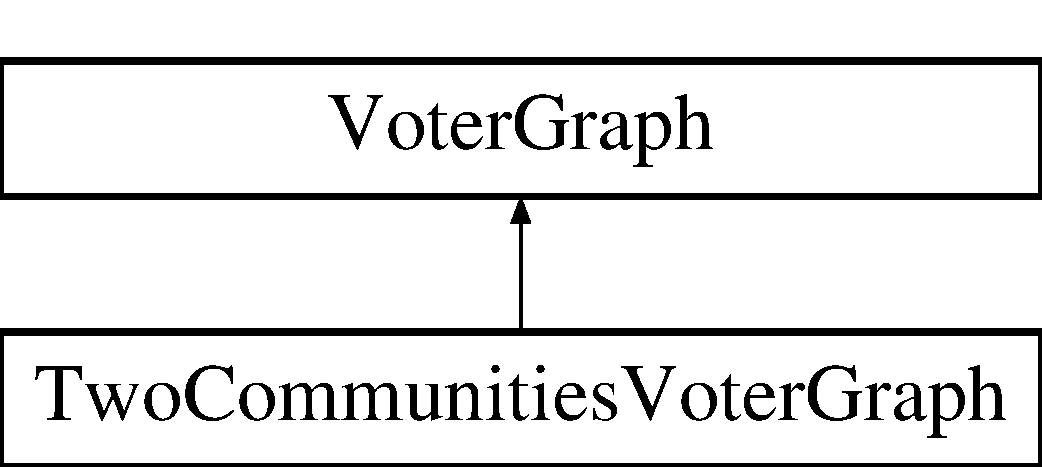
\includegraphics[height=2.000000cm]{class_two_communities_voter_graph}
\end{center}
\end{figure}
\subsection*{Public Member Functions}
\begin{DoxyCompactItemize}
\item 
\hyperlink{class_two_communities_voter_graph_a63c60c10b48a21413f7f60033448024e}{Two\-Communities\-Voter\-Graph} (int \hyperlink{class_two_communities_voter_graph_a3c9db0ac7e58d875ab3ce277bf74b284}{size1}, int \hyperlink{class_two_communities_voter_graph_a8b88457f020773b984e0d8c85d9ee502}{size2}, double \hyperlink{class_two_communities_voter_graph_a96a32ba7529177a7f6b73e827a57791e}{intra\-Rate1}, double \hyperlink{class_two_communities_voter_graph_a6e7ea06e014d75b7bf18441885e07e1e}{intra\-Rate2}, double \hyperlink{class_two_communities_voter_graph_af08c3b9a6e6f1dc8659a38ecd2d1afde}{inter\-Rate1}, double \hyperlink{class_two_communities_voter_graph_afab8bb5994f7fd1370d7d81caf7277d4}{inter\-Rate2}, double \hyperlink{class_two_communities_voter_graph_a883bf57bf07fb2e59f05df65df859a46}{contrarian1}, double \hyperlink{class_two_communities_voter_graph_a4274a05f5e2ceae57de1f0e71493b9a4}{contrarian2}, int update=\hyperlink{voter__graph_8hpp_ab3bec55c359e4ed771339c8bc61fc35aa01d100088352e1a7d3a34c9a66d0f951}{U\-P\-D\-A\-T\-E\-\_\-\-E\-D\-G\-E\-S})
\begin{DoxyCompactList}\small\item\em Constructor. \end{DoxyCompactList}\item 
\hypertarget{class_two_communities_voter_graph_ab74e186e76188e7de8ae11359ad1e55e}{\hyperlink{class_two_communities_voter_graph_ab74e186e76188e7de8ae11359ad1e55e}{$\sim$\-Two\-Communities\-Voter\-Graph} ()}\label{class_two_communities_voter_graph_ab74e186e76188e7de8ae11359ad1e55e}

\begin{DoxyCompactList}\small\item\em Destructor. \end{DoxyCompactList}\item 
\hyperlink{class_markov_process}{Markov\-Process} $\ast$ \hyperlink{class_two_communities_voter_graph_ac3e7b13e297275475e8f073ccfcac7d1}{get\-Compact\-Markov\-Process} ()
\begin{DoxyCompactList}\small\item\em Build the Markov chain associated to the graph, lumped according to the macro-\/state of community 1, the macro-\/state of community 2, and the state of the first agent in community 1. \end{DoxyCompactList}\item 
\hyperlink{class_partition}{Partition} $\ast$ \hyperlink{class_two_communities_voter_graph_a4dd6976ed1e02c761f6c4bd85bbf0f0c}{get\-Compact\-Markov\-Partition} (\hyperlink{class_voter_probe}{Voter\-Probe} $\ast$probe, \hyperlink{voter__graph_8hpp_acb4c45a5ce4a55eee28e54e60409b9c5}{Voter\-Metric} metric)
\begin{DoxyCompactList}\small\item\em Build the partition of the lumped Markov chain state space (see get\-Compact\-Markov\-Process) associated to a probe with a given metric (e.\-g., M\-E\-T\-R\-I\-C\-\_\-\-M\-A\-C\-R\-O\-\_\-\-S\-T\-A\-T\-E of M\-E\-T\-R\-I\-C\-\_\-\-A\-C\-T\-I\-V\-E\-\_\-\-E\-D\-G\-E\-S) \end{DoxyCompactList}\item 
\hyperlink{class_partition}{Partition} $\ast$ \hyperlink{class_two_communities_voter_graph_a13a1a7b219d0669f750a4281edf9aecf}{get\-Compact\-Markov\-Partition} (\hyperlink{class_voter_measurement}{Voter\-Measurement} $\ast$measurement)
\begin{DoxyCompactList}\small\item\em Build the partition of the lumped Markov chain state space (see get\-Compact\-Markov\-Process) associated to a measurement (i.\-e., a set of probes) \end{DoxyCompactList}\end{DoxyCompactItemize}
\subsection*{Public Attributes}
\begin{DoxyCompactItemize}
\item 
int \hyperlink{class_two_communities_voter_graph_a3c9db0ac7e58d875ab3ce277bf74b284}{size1}
\item 
int \hyperlink{class_two_communities_voter_graph_a8b88457f020773b984e0d8c85d9ee502}{size2}
\item 
double \hyperlink{class_two_communities_voter_graph_a96a32ba7529177a7f6b73e827a57791e}{intra\-Rate1}
\item 
double \hyperlink{class_two_communities_voter_graph_a6e7ea06e014d75b7bf18441885e07e1e}{intra\-Rate2}
\item 
double \hyperlink{class_two_communities_voter_graph_af08c3b9a6e6f1dc8659a38ecd2d1afde}{inter\-Rate1}
\item 
double \hyperlink{class_two_communities_voter_graph_afab8bb5994f7fd1370d7d81caf7277d4}{inter\-Rate2}
\item 
double \hyperlink{class_two_communities_voter_graph_a883bf57bf07fb2e59f05df65df859a46}{contrarian1}
\item 
double \hyperlink{class_two_communities_voter_graph_a4274a05f5e2ceae57de1f0e71493b9a4}{contrarian2}
\item 
std\-::set$<$ \hyperlink{class_voter_node}{Voter\-Node} $\ast$ $>$ $\ast$ \hyperlink{class_two_communities_voter_graph_a354768f44c0a3daa6d0a70a20df77af5}{community1}
\item 
std\-::set$<$ \hyperlink{class_voter_node}{Voter\-Node} $\ast$ $>$ $\ast$ \hyperlink{class_two_communities_voter_graph_a7c918c6733474caa86bc2d217bd2cb4d}{community2}
\end{DoxyCompactItemize}


\subsection{Detailed Description}
An interaction graph consisting in two communities of nodes (complete graph within each community, complete interaction between the two communities, possibly with different weights) 

\subsection{Constructor \& Destructor Documentation}
\hypertarget{class_two_communities_voter_graph_a63c60c10b48a21413f7f60033448024e}{\index{Two\-Communities\-Voter\-Graph@{Two\-Communities\-Voter\-Graph}!Two\-Communities\-Voter\-Graph@{Two\-Communities\-Voter\-Graph}}
\index{Two\-Communities\-Voter\-Graph@{Two\-Communities\-Voter\-Graph}!TwoCommunitiesVoterGraph@{Two\-Communities\-Voter\-Graph}}
\subsubsection[{Two\-Communities\-Voter\-Graph}]{\setlength{\rightskip}{0pt plus 5cm}Two\-Communities\-Voter\-Graph\-::\-Two\-Communities\-Voter\-Graph (
\begin{DoxyParamCaption}
\item[{int}]{size1, }
\item[{int}]{size2, }
\item[{double}]{intra\-Rate1, }
\item[{double}]{intra\-Rate2, }
\item[{double}]{inter\-Rate1, }
\item[{double}]{inter\-Rate2, }
\item[{double}]{contrarian1, }
\item[{double}]{contrarian2, }
\item[{int}]{update = {\ttfamily {\bf U\-P\-D\-A\-T\-E\-\_\-\-E\-D\-G\-E\-S}}}
\end{DoxyParamCaption}
)}}\label{class_two_communities_voter_graph_a63c60c10b48a21413f7f60033448024e}


Constructor. 


\begin{DoxyParams}{Parameters}
{\em size1} & \-: The size of community 1 \\
\hline
{\em size2} & \-: The size of community 2 \\
\hline
{\em intra\-Rate1} & \-: The weight of edges within community 1 \\
\hline
{\em intra\-Rate2} & \-: The weight of edges within community 2 \\
\hline
{\em inter\-Rate1} & \-: The weight of edges from community 1 to community 2 \\
\hline
{\em inter\-Rate2} & \-: The weight of edges from community 2 to community 1 \\
\hline
{\em contrarian1} & \-: The contrarian rate of nodes in community 1 \\
\hline
{\em contrarian2} & \-: The contrarian rate of nodes in community 2 \\
\hline
{\em update} & \-: How the system evolves at each simulation step (U\-P\-D\-A\-T\-E\-\_\-\-N\-O\-D\-E\-S or U\-P\-D\-A\-T\-E\-\_\-\-E\-D\-G\-E\-S) \\
\hline
\end{DoxyParams}


\subsection{Member Function Documentation}
\hypertarget{class_two_communities_voter_graph_a4dd6976ed1e02c761f6c4bd85bbf0f0c}{\index{Two\-Communities\-Voter\-Graph@{Two\-Communities\-Voter\-Graph}!get\-Compact\-Markov\-Partition@{get\-Compact\-Markov\-Partition}}
\index{get\-Compact\-Markov\-Partition@{get\-Compact\-Markov\-Partition}!TwoCommunitiesVoterGraph@{Two\-Communities\-Voter\-Graph}}
\subsubsection[{get\-Compact\-Markov\-Partition}]{\setlength{\rightskip}{0pt plus 5cm}{\bf Partition} $\ast$ Two\-Communities\-Voter\-Graph\-::get\-Compact\-Markov\-Partition (
\begin{DoxyParamCaption}
\item[{{\bf Voter\-Probe} $\ast$}]{probe, }
\item[{{\bf Voter\-Metric}}]{metric}
\end{DoxyParamCaption}
)}}\label{class_two_communities_voter_graph_a4dd6976ed1e02c761f6c4bd85bbf0f0c}


Build the partition of the lumped Markov chain state space (see get\-Compact\-Markov\-Process) associated to a probe with a given metric (e.\-g., M\-E\-T\-R\-I\-C\-\_\-\-M\-A\-C\-R\-O\-\_\-\-S\-T\-A\-T\-E of M\-E\-T\-R\-I\-C\-\_\-\-A\-C\-T\-I\-V\-E\-\_\-\-E\-D\-G\-E\-S) 


\begin{DoxyParams}{Parameters}
{\em probe} & \-: The probe used to partition the lumped state space \\
\hline
{\em metric} & \-: The metric of the probe (e.\-g., M\-E\-T\-R\-I\-C\-\_\-\-M\-A\-C\-R\-O\-\_\-\-S\-T\-A\-T\-E of M\-E\-T\-R\-I\-C\-\_\-\-A\-C\-T\-I\-V\-E\-\_\-\-E\-D\-G\-E\-S) \\
\hline
\end{DoxyParams}
\begin{DoxyReturn}{Returns}
The computed partition over the lumped state space 
\end{DoxyReturn}
\hypertarget{class_two_communities_voter_graph_a13a1a7b219d0669f750a4281edf9aecf}{\index{Two\-Communities\-Voter\-Graph@{Two\-Communities\-Voter\-Graph}!get\-Compact\-Markov\-Partition@{get\-Compact\-Markov\-Partition}}
\index{get\-Compact\-Markov\-Partition@{get\-Compact\-Markov\-Partition}!TwoCommunitiesVoterGraph@{Two\-Communities\-Voter\-Graph}}
\subsubsection[{get\-Compact\-Markov\-Partition}]{\setlength{\rightskip}{0pt plus 5cm}{\bf Partition} $\ast$ Two\-Communities\-Voter\-Graph\-::get\-Compact\-Markov\-Partition (
\begin{DoxyParamCaption}
\item[{{\bf Voter\-Measurement} $\ast$}]{measurement}
\end{DoxyParamCaption}
)}}\label{class_two_communities_voter_graph_a13a1a7b219d0669f750a4281edf9aecf}


Build the partition of the lumped Markov chain state space (see get\-Compact\-Markov\-Process) associated to a measurement (i.\-e., a set of probes) 


\begin{DoxyParams}{Parameters}
{\em measurement} & \-: The measurement used to partition the lumped state space \\
\hline
\end{DoxyParams}
\begin{DoxyReturn}{Returns}
The computed partition over the lumped state space 
\end{DoxyReturn}
\hypertarget{class_two_communities_voter_graph_ac3e7b13e297275475e8f073ccfcac7d1}{\index{Two\-Communities\-Voter\-Graph@{Two\-Communities\-Voter\-Graph}!get\-Compact\-Markov\-Process@{get\-Compact\-Markov\-Process}}
\index{get\-Compact\-Markov\-Process@{get\-Compact\-Markov\-Process}!TwoCommunitiesVoterGraph@{Two\-Communities\-Voter\-Graph}}
\subsubsection[{get\-Compact\-Markov\-Process}]{\setlength{\rightskip}{0pt plus 5cm}{\bf Markov\-Process} $\ast$ Two\-Communities\-Voter\-Graph\-::get\-Compact\-Markov\-Process (
\begin{DoxyParamCaption}
{}
\end{DoxyParamCaption}
)}}\label{class_two_communities_voter_graph_ac3e7b13e297275475e8f073ccfcac7d1}


Build the Markov chain associated to the graph, lumped according to the macro-\/state of community 1, the macro-\/state of community 2, and the state of the first agent in community 1. 

\begin{DoxyReturn}{Returns}
The computed lumped Markov chain 
\end{DoxyReturn}


\subsection{Member Data Documentation}
\hypertarget{class_two_communities_voter_graph_a354768f44c0a3daa6d0a70a20df77af5}{\index{Two\-Communities\-Voter\-Graph@{Two\-Communities\-Voter\-Graph}!community1@{community1}}
\index{community1@{community1}!TwoCommunitiesVoterGraph@{Two\-Communities\-Voter\-Graph}}
\subsubsection[{community1}]{\setlength{\rightskip}{0pt plus 5cm}std\-::set$<${\bf Voter\-Node}$\ast$$>$$\ast$ Two\-Communities\-Voter\-Graph\-::community1}}\label{class_two_communities_voter_graph_a354768f44c0a3daa6d0a70a20df77af5}
The set of nodes in community 1 \hypertarget{class_two_communities_voter_graph_a7c918c6733474caa86bc2d217bd2cb4d}{\index{Two\-Communities\-Voter\-Graph@{Two\-Communities\-Voter\-Graph}!community2@{community2}}
\index{community2@{community2}!TwoCommunitiesVoterGraph@{Two\-Communities\-Voter\-Graph}}
\subsubsection[{community2}]{\setlength{\rightskip}{0pt plus 5cm}std\-::set$<${\bf Voter\-Node}$\ast$$>$$\ast$ Two\-Communities\-Voter\-Graph\-::community2}}\label{class_two_communities_voter_graph_a7c918c6733474caa86bc2d217bd2cb4d}
The set of nodes in community 2 \hypertarget{class_two_communities_voter_graph_a883bf57bf07fb2e59f05df65df859a46}{\index{Two\-Communities\-Voter\-Graph@{Two\-Communities\-Voter\-Graph}!contrarian1@{contrarian1}}
\index{contrarian1@{contrarian1}!TwoCommunitiesVoterGraph@{Two\-Communities\-Voter\-Graph}}
\subsubsection[{contrarian1}]{\setlength{\rightskip}{0pt plus 5cm}double Two\-Communities\-Voter\-Graph\-::contrarian1}}\label{class_two_communities_voter_graph_a883bf57bf07fb2e59f05df65df859a46}
The contrarian rate of nodes in community 1 \hypertarget{class_two_communities_voter_graph_a4274a05f5e2ceae57de1f0e71493b9a4}{\index{Two\-Communities\-Voter\-Graph@{Two\-Communities\-Voter\-Graph}!contrarian2@{contrarian2}}
\index{contrarian2@{contrarian2}!TwoCommunitiesVoterGraph@{Two\-Communities\-Voter\-Graph}}
\subsubsection[{contrarian2}]{\setlength{\rightskip}{0pt plus 5cm}double Two\-Communities\-Voter\-Graph\-::contrarian2}}\label{class_two_communities_voter_graph_a4274a05f5e2ceae57de1f0e71493b9a4}
The contrarian rate of nodes in community 2 \hypertarget{class_two_communities_voter_graph_af08c3b9a6e6f1dc8659a38ecd2d1afde}{\index{Two\-Communities\-Voter\-Graph@{Two\-Communities\-Voter\-Graph}!inter\-Rate1@{inter\-Rate1}}
\index{inter\-Rate1@{inter\-Rate1}!TwoCommunitiesVoterGraph@{Two\-Communities\-Voter\-Graph}}
\subsubsection[{inter\-Rate1}]{\setlength{\rightskip}{0pt plus 5cm}double Two\-Communities\-Voter\-Graph\-::inter\-Rate1}}\label{class_two_communities_voter_graph_af08c3b9a6e6f1dc8659a38ecd2d1afde}
The weight of edges from community 1 to community 2 \hypertarget{class_two_communities_voter_graph_afab8bb5994f7fd1370d7d81caf7277d4}{\index{Two\-Communities\-Voter\-Graph@{Two\-Communities\-Voter\-Graph}!inter\-Rate2@{inter\-Rate2}}
\index{inter\-Rate2@{inter\-Rate2}!TwoCommunitiesVoterGraph@{Two\-Communities\-Voter\-Graph}}
\subsubsection[{inter\-Rate2}]{\setlength{\rightskip}{0pt plus 5cm}double Two\-Communities\-Voter\-Graph\-::inter\-Rate2}}\label{class_two_communities_voter_graph_afab8bb5994f7fd1370d7d81caf7277d4}
The weight of edges from community 2 to community 1 \hypertarget{class_two_communities_voter_graph_a96a32ba7529177a7f6b73e827a57791e}{\index{Two\-Communities\-Voter\-Graph@{Two\-Communities\-Voter\-Graph}!intra\-Rate1@{intra\-Rate1}}
\index{intra\-Rate1@{intra\-Rate1}!TwoCommunitiesVoterGraph@{Two\-Communities\-Voter\-Graph}}
\subsubsection[{intra\-Rate1}]{\setlength{\rightskip}{0pt plus 5cm}double Two\-Communities\-Voter\-Graph\-::intra\-Rate1}}\label{class_two_communities_voter_graph_a96a32ba7529177a7f6b73e827a57791e}
The weight of edges within community 1 \hypertarget{class_two_communities_voter_graph_a6e7ea06e014d75b7bf18441885e07e1e}{\index{Two\-Communities\-Voter\-Graph@{Two\-Communities\-Voter\-Graph}!intra\-Rate2@{intra\-Rate2}}
\index{intra\-Rate2@{intra\-Rate2}!TwoCommunitiesVoterGraph@{Two\-Communities\-Voter\-Graph}}
\subsubsection[{intra\-Rate2}]{\setlength{\rightskip}{0pt plus 5cm}double Two\-Communities\-Voter\-Graph\-::intra\-Rate2}}\label{class_two_communities_voter_graph_a6e7ea06e014d75b7bf18441885e07e1e}
The weight of edges within community 2 \hypertarget{class_two_communities_voter_graph_a3c9db0ac7e58d875ab3ce277bf74b284}{\index{Two\-Communities\-Voter\-Graph@{Two\-Communities\-Voter\-Graph}!size1@{size1}}
\index{size1@{size1}!TwoCommunitiesVoterGraph@{Two\-Communities\-Voter\-Graph}}
\subsubsection[{size1}]{\setlength{\rightskip}{0pt plus 5cm}int Two\-Communities\-Voter\-Graph\-::size1}}\label{class_two_communities_voter_graph_a3c9db0ac7e58d875ab3ce277bf74b284}
The size of community 1 \hypertarget{class_two_communities_voter_graph_a8b88457f020773b984e0d8c85d9ee502}{\index{Two\-Communities\-Voter\-Graph@{Two\-Communities\-Voter\-Graph}!size2@{size2}}
\index{size2@{size2}!TwoCommunitiesVoterGraph@{Two\-Communities\-Voter\-Graph}}
\subsubsection[{size2}]{\setlength{\rightskip}{0pt plus 5cm}int Two\-Communities\-Voter\-Graph\-::size2}}\label{class_two_communities_voter_graph_a8b88457f020773b984e0d8c85d9ee502}
The size of community 2 

The documentation for this class was generated from the following files\-:\begin{DoxyCompactItemize}
\item 
/home/lamarche/programming/multilevel\-\_\-prediction/src/\hyperlink{voter__graph_8hpp}{voter\-\_\-graph.\-hpp}\item 
/home/lamarche/programming/multilevel\-\_\-prediction/src/voter\-\_\-graph.\-cpp\end{DoxyCompactItemize}

\hypertarget{class_voter_binning}{\section{Voter\-Binning Class Reference}
\label{class_voter_binning}\index{Voter\-Binning@{Voter\-Binning}}
}
\subsection*{Public Member Functions}
\begin{DoxyCompactItemize}
\item 
\hypertarget{class_voter_binning_a4626ce3a1bb1aa2108afcfd63af89305}{{\bfseries Voter\-Binning} (\hyperlink{class_voter_data_set}{Voter\-Data\-Set} $\ast$data)}\label{class_voter_binning_a4626ce3a1bb1aa2108afcfd63af89305}

\item 
\hypertarget{class_voter_binning_acf647389a12d6e0838fec89eee8df72e}{void {\bfseries print} (bool verbose=false)}\label{class_voter_binning_acf647389a12d6e0838fec89eee8df72e}

\end{DoxyCompactItemize}
\subsection*{Public Attributes}
\begin{DoxyCompactItemize}
\item 
\hypertarget{class_voter_binning_abfb5cba676d4523a0db4253da90defd4}{\hyperlink{class_voter_data_set}{Voter\-Data\-Set} $\ast$ {\bfseries data}}\label{class_voter_binning_abfb5cba676d4523a0db4253da90defd4}

\item 
\hypertarget{class_voter_binning_a301ba12a243476ac1b7f7bdaa2bdf4b4}{int {\bfseries size}}\label{class_voter_binning_a301ba12a243476ac1b7f7bdaa2bdf4b4}

\item 
\hypertarget{class_voter_binning_a58e6aa4792f0b7f22794597742eb44a6}{int {\bfseries bin\-Number}}\label{class_voter_binning_a58e6aa4792f0b7f22794597742eb44a6}

\item 
\hypertarget{class_voter_binning_a5226a976c3ac9a43e9ed485d9de2712a}{int $\ast$ {\bfseries cuts}}\label{class_voter_binning_a5226a976c3ac9a43e9ed485d9de2712a}

\item 
\hypertarget{class_voter_binning_a9d385619fee2689a5530cc8e06f44d37}{double {\bfseries score}}\label{class_voter_binning_a9d385619fee2689a5530cc8e06f44d37}

\end{DoxyCompactItemize}


The documentation for this class was generated from the following files\-:\begin{DoxyCompactItemize}
\item 
/home/lamarche/programming/multilevel\-\_\-prediction/src/\hyperlink{voter__graph_8hpp}{voter\-\_\-graph.\-hpp}\item 
/home/lamarche/programming/multilevel\-\_\-prediction/src/voter\-\_\-graph.\-cpp\end{DoxyCompactItemize}

\hypertarget{class_voter_data_set}{\section{Voter\-Data\-Set Class Reference}
\label{class_voter_data_set}\index{Voter\-Data\-Set@{Voter\-Data\-Set}}
}
\subsection*{Public Member Functions}
\begin{DoxyCompactItemize}
\item 
\hypertarget{class_voter_data_set_a85862f252fad49f884e47db2f5a5674c}{{\bfseries Voter\-Data\-Set} (\hyperlink{class_voter_graph}{Voter\-Graph} $\ast$graph, int time, int delay, int train\-Size, int test\-Size, int train\-Length, int test\-Length)}\label{class_voter_data_set_a85862f252fad49f884e47db2f5a5674c}

\item 
\hypertarget{class_voter_data_set_af70ae2bf803da48a2d9e8d63fe3ff734}{void {\bfseries estimate\-Transition\-Map} (\hyperlink{class_voter_measurement}{Voter\-Measurement} $\ast$pre\-M, \hyperlink{class_voter_measurement}{Voter\-Measurement} $\ast$post\-M)}\label{class_voter_data_set_af70ae2bf803da48a2d9e8d63fe3ff734}

\item 
\hypertarget{class_voter_data_set_ad012aba1d9993327593f7cddc325d51c}{void {\bfseries print\-Transition\-Map} ()}\label{class_voter_data_set_ad012aba1d9993327593f7cddc325d51c}

\item 
\hypertarget{class_voter_data_set_a2a979b77b09ed30a92335423ebe21d12}{double {\bfseries get\-Log\-Score} (\hyperlink{class_voter_measurement}{Voter\-Measurement} $\ast$pre\-M, \hyperlink{class_voter_measurement}{Voter\-Measurement} $\ast$post\-M, int prior=0)}\label{class_voter_data_set_a2a979b77b09ed30a92335423ebe21d12}

\item 
\hypertarget{class_voter_data_set_a5c641ff7d0ce7a150ef8ebd46bc4da5e}{double {\bfseries get\-Quad\-Score} (\hyperlink{class_voter_measurement}{Voter\-Measurement} $\ast$pre\-M, \hyperlink{class_voter_measurement}{Voter\-Measurement} $\ast$post\-M, int prior=0)}\label{class_voter_data_set_a5c641ff7d0ce7a150ef8ebd46bc4da5e}

\item 
\hypertarget{class_voter_data_set_aaab30a1a42a992b61a66107353bb89c6}{\hyperlink{class_voter_binning}{Voter\-Binning} $\ast$ {\bfseries get\-Optimal\-Binning} (\hyperlink{class_voter_measurement}{Voter\-Measurement} $\ast$pre\-M, \hyperlink{class_voter_measurement}{Voter\-Measurement} $\ast$post\-M, int prior=0, int real\-Train\-Size=-\/1, bool verbose=false)}\label{class_voter_data_set_aaab30a1a42a992b61a66107353bb89c6}

\end{DoxyCompactItemize}
\subsection*{Public Attributes}
\begin{DoxyCompactItemize}
\item 
\hypertarget{class_voter_data_set_afc4d76589e0112bb5c8e30730074231e}{\hyperlink{class_voter_graph}{Voter\-Graph} $\ast$ {\bfseries graph}}\label{class_voter_data_set_afc4d76589e0112bb5c8e30730074231e}

\item 
\hypertarget{class_voter_data_set_a50a2e44a9d6d99d3254e3da816f76aff}{int {\bfseries time}}\label{class_voter_data_set_a50a2e44a9d6d99d3254e3da816f76aff}

\item 
\hypertarget{class_voter_data_set_a32c0fb1d14c53d2c10a28463f9e44a7f}{int {\bfseries delay}}\label{class_voter_data_set_a32c0fb1d14c53d2c10a28463f9e44a7f}

\item 
\hypertarget{class_voter_data_set_a8aadcc50a4094f7d43f3172c70ae5f73}{int {\bfseries train\-Size}}\label{class_voter_data_set_a8aadcc50a4094f7d43f3172c70ae5f73}

\item 
\hypertarget{class_voter_data_set_a068aae3fc53a52217cc9014ba21090dd}{int {\bfseries test\-Size}}\label{class_voter_data_set_a068aae3fc53a52217cc9014ba21090dd}

\item 
\hypertarget{class_voter_data_set_ad7cb5062b8c67a26ee50939d54027748}{int {\bfseries train\-Length}}\label{class_voter_data_set_ad7cb5062b8c67a26ee50939d54027748}

\item 
\hypertarget{class_voter_data_set_a89ce0e2c44631818736ca7f71056f6c0}{int {\bfseries test\-Length}}\label{class_voter_data_set_a89ce0e2c44631818736ca7f71056f6c0}

\item 
\hypertarget{class_voter_data_set_a07299f2883a8ec069d9821a877351725}{\hyperlink{class_voter_trajectory}{Voter\-Trajectory} $\ast$$\ast$ {\bfseries trajectories}}\label{class_voter_data_set_a07299f2883a8ec069d9821a877351725}

\item 
\hypertarget{class_voter_data_set_a0f0ee88cf6290a0a679982a5fef315b0}{Transition\-Map $\ast$ {\bfseries trans\-Map}}\label{class_voter_data_set_a0f0ee88cf6290a0a679982a5fef315b0}

\end{DoxyCompactItemize}


The documentation for this class was generated from the following files\-:\begin{DoxyCompactItemize}
\item 
/home/lamarche/programming/multilevel\-\_\-prediction/src/\hyperlink{voter__graph_8hpp}{voter\-\_\-graph.\-hpp}\item 
/home/lamarche/programming/multilevel\-\_\-prediction/src/voter\-\_\-graph.\-cpp\end{DoxyCompactItemize}

\hypertarget{class_voter_edge}{}\section{Voter\+Edge Class Reference}
\label{class_voter_edge}\index{Voter\+Edge@{Voter\+Edge}}


An edge of the interaction graph.  




{\ttfamily \#include $<$voter\+\_\+graph.\+hpp$>$}

\subsection*{Public Member Functions}
\begin{DoxyCompactItemize}
\item 
\hyperlink{class_voter_edge_aba882697ef6b0a859a6842d378b589e1}{Voter\+Edge} (\hyperlink{class_voter_node}{Voter\+Node} $\ast$\hyperlink{class_voter_edge_aaa3e4febee48a905652ba142b8a48b7e}{node1}, \hyperlink{class_voter_node}{Voter\+Node} $\ast$\hyperlink{class_voter_edge_a2483bd0524c590213c0abd33f7a5de2b}{node2}, double \hyperlink{class_voter_edge_a08b1042475d9628a0da0e7ebf8557923}{weight}=1)
\begin{DoxyCompactList}\small\item\em Constructor. \end{DoxyCompactList}\item 
\hypertarget{class_voter_edge_a65882f301c4f20f229e5413c4212ce0c}{}\hyperlink{class_voter_edge_a65882f301c4f20f229e5413c4212ce0c}{$\sim$\+Voter\+Edge} ()\label{class_voter_edge_a65882f301c4f20f229e5413c4212ce0c}

\begin{DoxyCompactList}\small\item\em Destructor. \end{DoxyCompactList}\end{DoxyCompactItemize}
\subsection*{Public Attributes}
\begin{DoxyCompactItemize}
\item 
\hyperlink{class_voter_node}{Voter\+Node} $\ast$ \hyperlink{class_voter_edge_aaa3e4febee48a905652ba142b8a48b7e}{node1}
\item 
\hyperlink{class_voter_node}{Voter\+Node} $\ast$ \hyperlink{class_voter_edge_a2483bd0524c590213c0abd33f7a5de2b}{node2}
\item 
double \hyperlink{class_voter_edge_a08b1042475d9628a0da0e7ebf8557923}{weight}
\end{DoxyCompactItemize}


\subsection{Detailed Description}
An edge of the interaction graph. 

\subsection{Constructor \& Destructor Documentation}
\hypertarget{class_voter_edge_aba882697ef6b0a859a6842d378b589e1}{}\index{Voter\+Edge@{Voter\+Edge}!Voter\+Edge@{Voter\+Edge}}
\index{Voter\+Edge@{Voter\+Edge}!Voter\+Edge@{Voter\+Edge}}
\subsubsection[{Voter\+Edge}]{\setlength{\rightskip}{0pt plus 5cm}Voter\+Edge\+::\+Voter\+Edge (
\begin{DoxyParamCaption}
\item[{{\bf Voter\+Node} $\ast$}]{node1, }
\item[{{\bf Voter\+Node} $\ast$}]{node2, }
\item[{double}]{weight = {\ttfamily 1}}
\end{DoxyParamCaption}
)}\label{class_voter_edge_aba882697ef6b0a859a6842d378b589e1}


Constructor. 


\begin{DoxyParams}{Parameters}
{\em node1} & \+: Incoming node \\
\hline
{\em node2} & \+: Outcoming node \\
\hline
{\em weight} & \+: Determines the probability to select this edge (relatively to other edges) at each simulation step when the update\+Process variable of the graph is set to U\+P\+D\+A\+T\+E\+\_\+\+E\+D\+G\+E\+S \\
\hline
\end{DoxyParams}


\subsection{Member Data Documentation}
\hypertarget{class_voter_edge_aaa3e4febee48a905652ba142b8a48b7e}{}\index{Voter\+Edge@{Voter\+Edge}!node1@{node1}}
\index{node1@{node1}!Voter\+Edge@{Voter\+Edge}}
\subsubsection[{node1}]{\setlength{\rightskip}{0pt plus 5cm}{\bf Voter\+Node}$\ast$ Voter\+Edge\+::node1}\label{class_voter_edge_aaa3e4febee48a905652ba142b8a48b7e}
Incoming node \hypertarget{class_voter_edge_a2483bd0524c590213c0abd33f7a5de2b}{}\index{Voter\+Edge@{Voter\+Edge}!node2@{node2}}
\index{node2@{node2}!Voter\+Edge@{Voter\+Edge}}
\subsubsection[{node2}]{\setlength{\rightskip}{0pt plus 5cm}{\bf Voter\+Node}$\ast$ Voter\+Edge\+::node2}\label{class_voter_edge_a2483bd0524c590213c0abd33f7a5de2b}
Outcoming node \hypertarget{class_voter_edge_a08b1042475d9628a0da0e7ebf8557923}{}\index{Voter\+Edge@{Voter\+Edge}!weight@{weight}}
\index{weight@{weight}!Voter\+Edge@{Voter\+Edge}}
\subsubsection[{weight}]{\setlength{\rightskip}{0pt plus 5cm}double Voter\+Edge\+::weight}\label{class_voter_edge_a08b1042475d9628a0da0e7ebf8557923}
Determines the probability to select this edge (relatively to other edges) at each simulation step when the update\+Process variable of the graph is set to U\+P\+D\+A\+T\+E\+\_\+\+E\+D\+G\+E\+S 

The documentation for this class was generated from the following files\+:\begin{DoxyCompactItemize}
\item 
C\+:/\+Users/\+Robin/\+Mes projets/programming/multilevel\+\_\+prediction/src/\hyperlink{voter__graph_8hpp}{voter\+\_\+graph.\+hpp}\item 
C\+:/\+Users/\+Robin/\+Mes projets/programming/multilevel\+\_\+prediction/src/voter\+\_\+graph.\+cpp\end{DoxyCompactItemize}

\hypertarget{class_voter_graph}{}\section{Voter\+Graph Class Reference}
\label{class_voter_graph}\index{Voter\+Graph@{Voter\+Graph}}


The interaction graph describing a Voter Model.  




{\ttfamily \#include $<$voter\+\_\+graph.\+hpp$>$}

Inheritance diagram for Voter\+Graph\+:\begin{figure}[H]
\begin{center}
\leavevmode
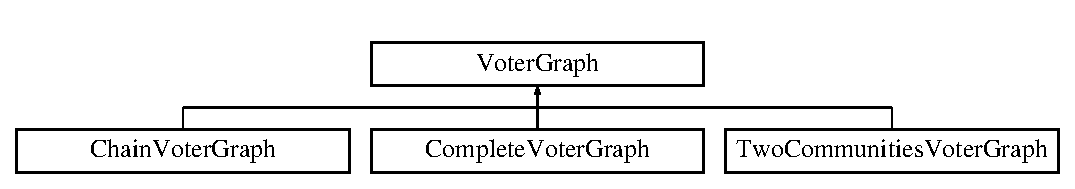
\includegraphics[height=2.000000cm]{class_voter_graph}
\end{center}
\end{figure}
\subsection*{Public Member Functions}
\begin{DoxyCompactItemize}
\item 
\hyperlink{class_voter_graph_aa5e00e0f2d2d8de10a217633d4594814}{Voter\+Graph} (int update=\hyperlink{voter__graph_8hpp_a305d80651467e931f258a3686976d31c}{U\+P\+D\+A\+T\+E\+\_\+\+E\+D\+G\+E\+S})
\begin{DoxyCompactList}\small\item\em Constructor. \end{DoxyCompactList}\item 
\hypertarget{class_voter_graph_a84a3f081c6e15cf8d1635d6ee6d5e51e}{}\hyperlink{class_voter_graph_a84a3f081c6e15cf8d1635d6ee6d5e51e}{$\sim$\+Voter\+Graph} ()\label{class_voter_graph_a84a3f081c6e15cf8d1635d6ee6d5e51e}

\begin{DoxyCompactList}\small\item\em Destructor. \end{DoxyCompactList}\item 
\hypertarget{class_voter_graph_aacb7bbd4bcc7f923b2784b0bcefcd1a3}{}void \hyperlink{class_voter_graph_aacb7bbd4bcc7f923b2784b0bcefcd1a3}{print} ()\label{class_voter_graph_aacb7bbd4bcc7f923b2784b0bcefcd1a3}

\begin{DoxyCompactList}\small\item\em Print the graph. \end{DoxyCompactList}\item 
\hyperlink{class_voter_node}{Voter\+Node} $\ast$ \hyperlink{class_voter_graph_af53017970f3ac08838b67f4a09171b92}{add\+Node} (double weight=1, double contrarian=0)
\begin{DoxyCompactList}\small\item\em Add a node to the graph. \end{DoxyCompactList}\item 
\hyperlink{class_voter_edge}{Voter\+Edge} $\ast$ \hyperlink{class_voter_graph_a1f6b8be82800577c45908102251f1e35}{add\+Edge} (\hyperlink{class_voter_node}{Voter\+Node} $\ast$node1, \hyperlink{class_voter_node}{Voter\+Node} $\ast$node2, double weight=1)
\begin{DoxyCompactList}\small\item\em Add an edge to the graph. \end{DoxyCompactList}\item 
\hypertarget{class_voter_graph_aa86a23e7d5984c3c6bbea76f193b73ae}{}void \hyperlink{class_voter_graph_aa86a23e7d5984c3c6bbea76f193b73ae}{fill\+Edges} ()\label{class_voter_graph_aa86a23e7d5984c3c6bbea76f193b73ae}

\begin{DoxyCompactList}\small\item\em Add an edge between each pair of nodes in the graph (in both direction, with equal weight for each edge) \end{DoxyCompactList}\item 
\hyperlink{class_markov_process}{Markov\+Process} $\ast$ \hyperlink{class_voter_graph_acc86929339ec0a0ce2946146919b1eb7}{get\+Markov\+Process} ()
\begin{DoxyCompactList}\small\item\em Build the Markov chain associated to the described Voter Model. \end{DoxyCompactList}\item 
\hyperlink{class_partition}{Partition} $\ast$ \hyperlink{class_voter_graph_a2303b38ee1a599554f730236d9f4fc7c}{get\+Markov\+Partition} (\hyperlink{class_voter_probe}{Voter\+Probe} $\ast$probe, int metric)
\begin{DoxyCompactList}\small\item\em Build the partition of the Markov chain state space associated to a probe with a given metric (e.\+g., M\+E\+T\+R\+I\+C\+\_\+\+M\+A\+C\+R\+O\+\_\+\+S\+T\+A\+T\+E of M\+E\+T\+R\+I\+C\+\_\+\+A\+C\+T\+I\+V\+E\+\_\+\+E\+D\+G\+E\+S) \end{DoxyCompactList}\item 
\hyperlink{class_partition}{Partition} $\ast$ \hyperlink{class_voter_graph_a2c0a299c1249cc04e011d0f507467007}{get\+Markov\+Partition} (\hyperlink{class_voter_measurement}{Voter\+Measurement} $\ast$measurement)
\begin{DoxyCompactList}\small\item\em Build the partition of the Markov chain state space associated to a measurement (i.\+e., a set of probes) \end{DoxyCompactList}\end{DoxyCompactItemize}
\subsection*{Public Attributes}
\begin{DoxyCompactItemize}
\item 
int \hyperlink{class_voter_graph_a11db0ef474064d44adb3ea22df8199ee}{update\+Process}
\item 
int \hyperlink{class_voter_graph_a7557cf918e298cf5d5558f7323fe8f35}{node\+Number}
\item 
int \hyperlink{class_voter_graph_a6840594abf9c606b4ac8c7cac88cdf9b}{edge\+Number}
\item 
double \hyperlink{class_voter_graph_a8108f0b182d1ca41ef567f7b729fe749}{node\+Weight}
\item 
double \hyperlink{class_voter_graph_a33dc5727bd80818f0d4e89c17303d7c8}{edge\+Weight}
\item 
std\+::map$<$ int, \hyperlink{class_voter_node}{Voter\+Node} $\ast$ $>$ $\ast$ \hyperlink{class_voter_graph_a73838569fae5c5c96efadb1f121f5a90}{node\+Map}
\item 
std\+::set$<$ \hyperlink{class_voter_node}{Voter\+Node} $\ast$ $>$ $\ast$ \hyperlink{class_voter_graph_ab4c1bdbd12ebccd735841471984dfeec}{node\+Set}
\item 
std\+::set$<$ \hyperlink{class_voter_edge}{Voter\+Edge} $\ast$ $>$ $\ast$ \hyperlink{class_voter_graph_a712b0ec4b780579721b7b6bca8fd409e}{edge\+Set}
\item 
\hyperlink{class_markov_process}{Markov\+Process} $\ast$ \hyperlink{class_voter_graph_a94b668c67f423d3a4ce25d5605a467cb}{process}
\end{DoxyCompactItemize}


\subsection{Detailed Description}
The interaction graph describing a Voter Model. 

\subsection{Constructor \& Destructor Documentation}
\hypertarget{class_voter_graph_aa5e00e0f2d2d8de10a217633d4594814}{}\index{Voter\+Graph@{Voter\+Graph}!Voter\+Graph@{Voter\+Graph}}
\index{Voter\+Graph@{Voter\+Graph}!Voter\+Graph@{Voter\+Graph}}
\subsubsection[{Voter\+Graph}]{\setlength{\rightskip}{0pt plus 5cm}Voter\+Graph\+::\+Voter\+Graph (
\begin{DoxyParamCaption}
\item[{int}]{update = {\ttfamily {\bf U\+P\+D\+A\+T\+E\+\_\+\+E\+D\+G\+E\+S}}}
\end{DoxyParamCaption}
)}\label{class_voter_graph_aa5e00e0f2d2d8de10a217633d4594814}


Constructor. 


\begin{DoxyParams}{Parameters}
{\em update} & \+: How the system evolves at each simulation step (U\+P\+D\+A\+T\+E\+\_\+\+N\+O\+D\+E\+S or U\+P\+D\+A\+T\+E\+\_\+\+E\+D\+G\+E\+S) \\
\hline
\end{DoxyParams}


\subsection{Member Function Documentation}
\hypertarget{class_voter_graph_a1f6b8be82800577c45908102251f1e35}{}\index{Voter\+Graph@{Voter\+Graph}!add\+Edge@{add\+Edge}}
\index{add\+Edge@{add\+Edge}!Voter\+Graph@{Voter\+Graph}}
\subsubsection[{add\+Edge}]{\setlength{\rightskip}{0pt plus 5cm}{\bf Voter\+Edge} $\ast$ Voter\+Graph\+::add\+Edge (
\begin{DoxyParamCaption}
\item[{{\bf Voter\+Node} $\ast$}]{node1, }
\item[{{\bf Voter\+Node} $\ast$}]{node2, }
\item[{double}]{weight = {\ttfamily 1}}
\end{DoxyParamCaption}
)}\label{class_voter_graph_a1f6b8be82800577c45908102251f1e35}


Add an edge to the graph. 


\begin{DoxyParams}{Parameters}
{\em node1} & \+: Incoming node \\
\hline
{\em node2} & \+: outcoming node \\
\hline
{\em weight} & \+: Determines the probability to select the edge to be added (relatively to other edges) at each simulation step when the update\+Process variable of the graph is set to U\+P\+D\+A\+T\+E\+\_\+\+E\+D\+G\+E\+S \\
\hline
\end{DoxyParams}
\begin{DoxyReturn}{Returns}
The added edge 
\end{DoxyReturn}
\hypertarget{class_voter_graph_af53017970f3ac08838b67f4a09171b92}{}\index{Voter\+Graph@{Voter\+Graph}!add\+Node@{add\+Node}}
\index{add\+Node@{add\+Node}!Voter\+Graph@{Voter\+Graph}}
\subsubsection[{add\+Node}]{\setlength{\rightskip}{0pt plus 5cm}{\bf Voter\+Node} $\ast$ Voter\+Graph\+::add\+Node (
\begin{DoxyParamCaption}
\item[{double}]{weight = {\ttfamily 1}, }
\item[{double}]{contrarian = {\ttfamily 0}}
\end{DoxyParamCaption}
)}\label{class_voter_graph_af53017970f3ac08838b67f4a09171b92}


Add a node to the graph. 


\begin{DoxyParams}{Parameters}
{\em weight} & \+: Determines the probability to select the node to be added (relatively to other nodes) at each simulation step when the update\+Process variable of the graph is set to U\+P\+D\+A\+T\+E\+\_\+\+N\+O\+D\+E\+S \\
\hline
{\em contrarian} & \+: The contrarian rate of the node to be added \\
\hline
\end{DoxyParams}
\begin{DoxyReturn}{Returns}
The added node 
\end{DoxyReturn}
\hypertarget{class_voter_graph_a2303b38ee1a599554f730236d9f4fc7c}{}\index{Voter\+Graph@{Voter\+Graph}!get\+Markov\+Partition@{get\+Markov\+Partition}}
\index{get\+Markov\+Partition@{get\+Markov\+Partition}!Voter\+Graph@{Voter\+Graph}}
\subsubsection[{get\+Markov\+Partition}]{\setlength{\rightskip}{0pt plus 5cm}{\bf Partition} $\ast$ Voter\+Graph\+::get\+Markov\+Partition (
\begin{DoxyParamCaption}
\item[{{\bf Voter\+Probe} $\ast$}]{probe, }
\item[{int}]{metric}
\end{DoxyParamCaption}
)}\label{class_voter_graph_a2303b38ee1a599554f730236d9f4fc7c}


Build the partition of the Markov chain state space associated to a probe with a given metric (e.\+g., M\+E\+T\+R\+I\+C\+\_\+\+M\+A\+C\+R\+O\+\_\+\+S\+T\+A\+T\+E of M\+E\+T\+R\+I\+C\+\_\+\+A\+C\+T\+I\+V\+E\+\_\+\+E\+D\+G\+E\+S) 


\begin{DoxyParams}{Parameters}
{\em probe} & \+: The probe used to partition the state space \\
\hline
{\em metric} & \+: The metric of the probe (e.\+g., M\+E\+T\+R\+I\+C\+\_\+\+M\+A\+C\+R\+O\+\_\+\+S\+T\+A\+T\+E of M\+E\+T\+R\+I\+C\+\_\+\+A\+C\+T\+I\+V\+E\+\_\+\+E\+D\+G\+E\+S) \\
\hline
\end{DoxyParams}
\begin{DoxyReturn}{Returns}
The computed partition 
\end{DoxyReturn}
\hypertarget{class_voter_graph_a2c0a299c1249cc04e011d0f507467007}{}\index{Voter\+Graph@{Voter\+Graph}!get\+Markov\+Partition@{get\+Markov\+Partition}}
\index{get\+Markov\+Partition@{get\+Markov\+Partition}!Voter\+Graph@{Voter\+Graph}}
\subsubsection[{get\+Markov\+Partition}]{\setlength{\rightskip}{0pt plus 5cm}{\bf Partition} $\ast$ Voter\+Graph\+::get\+Markov\+Partition (
\begin{DoxyParamCaption}
\item[{{\bf Voter\+Measurement} $\ast$}]{measurement}
\end{DoxyParamCaption}
)}\label{class_voter_graph_a2c0a299c1249cc04e011d0f507467007}


Build the partition of the Markov chain state space associated to a measurement (i.\+e., a set of probes) 


\begin{DoxyParams}{Parameters}
{\em measurement} & \+: The measurement used to partition the state space \\
\hline
\end{DoxyParams}
\begin{DoxyReturn}{Returns}
The computed partition 
\end{DoxyReturn}
\hypertarget{class_voter_graph_acc86929339ec0a0ce2946146919b1eb7}{}\index{Voter\+Graph@{Voter\+Graph}!get\+Markov\+Process@{get\+Markov\+Process}}
\index{get\+Markov\+Process@{get\+Markov\+Process}!Voter\+Graph@{Voter\+Graph}}
\subsubsection[{get\+Markov\+Process}]{\setlength{\rightskip}{0pt plus 5cm}{\bf Markov\+Process} $\ast$ Voter\+Graph\+::get\+Markov\+Process (
\begin{DoxyParamCaption}
{}
\end{DoxyParamCaption}
)}\label{class_voter_graph_acc86929339ec0a0ce2946146919b1eb7}


Build the Markov chain associated to the described Voter Model. 

\begin{DoxyReturn}{Returns}
The computed Markov chain 
\end{DoxyReturn}


\subsection{Member Data Documentation}
\hypertarget{class_voter_graph_a6840594abf9c606b4ac8c7cac88cdf9b}{}\index{Voter\+Graph@{Voter\+Graph}!edge\+Number@{edge\+Number}}
\index{edge\+Number@{edge\+Number}!Voter\+Graph@{Voter\+Graph}}
\subsubsection[{edge\+Number}]{\setlength{\rightskip}{0pt plus 5cm}int Voter\+Graph\+::edge\+Number}\label{class_voter_graph_a6840594abf9c606b4ac8c7cac88cdf9b}
The total number of edges in the graph \hypertarget{class_voter_graph_a712b0ec4b780579721b7b6bca8fd409e}{}\index{Voter\+Graph@{Voter\+Graph}!edge\+Set@{edge\+Set}}
\index{edge\+Set@{edge\+Set}!Voter\+Graph@{Voter\+Graph}}
\subsubsection[{edge\+Set}]{\setlength{\rightskip}{0pt plus 5cm}std\+::set$<${\bf Voter\+Edge}$\ast$$>$$\ast$ Voter\+Graph\+::edge\+Set}\label{class_voter_graph_a712b0ec4b780579721b7b6bca8fd409e}
The set of all edges \hypertarget{class_voter_graph_a33dc5727bd80818f0d4e89c17303d7c8}{}\index{Voter\+Graph@{Voter\+Graph}!edge\+Weight@{edge\+Weight}}
\index{edge\+Weight@{edge\+Weight}!Voter\+Graph@{Voter\+Graph}}
\subsubsection[{edge\+Weight}]{\setlength{\rightskip}{0pt plus 5cm}double Voter\+Graph\+::edge\+Weight}\label{class_voter_graph_a33dc5727bd80818f0d4e89c17303d7c8}
The sum of the weight of all edges \hypertarget{class_voter_graph_a73838569fae5c5c96efadb1f121f5a90}{}\index{Voter\+Graph@{Voter\+Graph}!node\+Map@{node\+Map}}
\index{node\+Map@{node\+Map}!Voter\+Graph@{Voter\+Graph}}
\subsubsection[{node\+Map}]{\setlength{\rightskip}{0pt plus 5cm}std\+::map$<$int,{\bf Voter\+Node}$\ast$$>$$\ast$ Voter\+Graph\+::node\+Map}\label{class_voter_graph_a73838569fae5c5c96efadb1f121f5a90}
The map of all nodes organized by id \hypertarget{class_voter_graph_a7557cf918e298cf5d5558f7323fe8f35}{}\index{Voter\+Graph@{Voter\+Graph}!node\+Number@{node\+Number}}
\index{node\+Number@{node\+Number}!Voter\+Graph@{Voter\+Graph}}
\subsubsection[{node\+Number}]{\setlength{\rightskip}{0pt plus 5cm}int Voter\+Graph\+::node\+Number}\label{class_voter_graph_a7557cf918e298cf5d5558f7323fe8f35}
The total number of nodes in the graph \hypertarget{class_voter_graph_ab4c1bdbd12ebccd735841471984dfeec}{}\index{Voter\+Graph@{Voter\+Graph}!node\+Set@{node\+Set}}
\index{node\+Set@{node\+Set}!Voter\+Graph@{Voter\+Graph}}
\subsubsection[{node\+Set}]{\setlength{\rightskip}{0pt plus 5cm}std\+::set$<${\bf Voter\+Node}$\ast$$>$$\ast$ Voter\+Graph\+::node\+Set}\label{class_voter_graph_ab4c1bdbd12ebccd735841471984dfeec}
The set of all nodes \hypertarget{class_voter_graph_a8108f0b182d1ca41ef567f7b729fe749}{}\index{Voter\+Graph@{Voter\+Graph}!node\+Weight@{node\+Weight}}
\index{node\+Weight@{node\+Weight}!Voter\+Graph@{Voter\+Graph}}
\subsubsection[{node\+Weight}]{\setlength{\rightskip}{0pt plus 5cm}double Voter\+Graph\+::node\+Weight}\label{class_voter_graph_a8108f0b182d1ca41ef567f7b729fe749}
The sum of the weight of all nodes \hypertarget{class_voter_graph_a94b668c67f423d3a4ce25d5605a467cb}{}\index{Voter\+Graph@{Voter\+Graph}!process@{process}}
\index{process@{process}!Voter\+Graph@{Voter\+Graph}}
\subsubsection[{process}]{\setlength{\rightskip}{0pt plus 5cm}{\bf Markov\+Process}$\ast$ Voter\+Graph\+::process}\label{class_voter_graph_a94b668c67f423d3a4ce25d5605a467cb}
The Markov chain associated to the described Voter Model \hypertarget{class_voter_graph_a11db0ef474064d44adb3ea22df8199ee}{}\index{Voter\+Graph@{Voter\+Graph}!update\+Process@{update\+Process}}
\index{update\+Process@{update\+Process}!Voter\+Graph@{Voter\+Graph}}
\subsubsection[{update\+Process}]{\setlength{\rightskip}{0pt plus 5cm}int Voter\+Graph\+::update\+Process}\label{class_voter_graph_a11db0ef474064d44adb3ea22df8199ee}
How the system evolves at each simulation step (U\+P\+D\+A\+T\+E\+\_\+\+N\+O\+D\+E\+S or U\+P\+D\+A\+T\+E\+\_\+\+E\+D\+G\+E\+S) 

The documentation for this class was generated from the following files\+:\begin{DoxyCompactItemize}
\item 
C\+:/\+Users/\+Robin/\+Mes projets/programming/multilevel\+\_\+prediction/src/\hyperlink{voter__graph_8hpp}{voter\+\_\+graph.\+hpp}\item 
C\+:/\+Users/\+Robin/\+Mes projets/programming/multilevel\+\_\+prediction/src/voter\+\_\+graph.\+cpp\end{DoxyCompactItemize}

\hypertarget{class_voter_measurement}{\section{Voter\-Measurement Class Reference}
\label{class_voter_measurement}\index{Voter\-Measurement@{Voter\-Measurement}}
}


A measurement to observe the Voter Model according set of probes.  




{\ttfamily \#include $<$voter\-\_\-graph.\-hpp$>$}

Inheritance diagram for Voter\-Measurement\-:\begin{figure}[H]
\begin{center}
\leavevmode
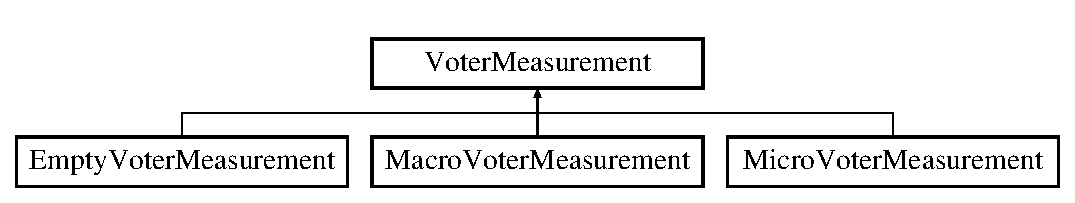
\includegraphics[height=2.000000cm]{class_voter_measurement}
\end{center}
\end{figure}
\subsection*{Public Member Functions}
\begin{DoxyCompactItemize}
\item 
\hyperlink{class_voter_measurement_a0668249876e48af0ae246a554b30195c}{Voter\-Measurement} (\hyperlink{class_voter_graph}{Voter\-Graph} $\ast$\hyperlink{class_voter_measurement_a8d22d4b78f7e2f4c747f5716c4885351}{graph}, std\-::string \hyperlink{class_voter_measurement_ad4471a133827f052622a84c4a451aabe}{type})
\begin{DoxyCompactList}\small\item\em Constructor. \end{DoxyCompactList}\item 
\hypertarget{class_voter_measurement_a2cbd2d015fad1579c21dc62dd2511fe6}{\hyperlink{class_voter_measurement_a2cbd2d015fad1579c21dc62dd2511fe6}{$\sim$\-Voter\-Measurement} ()}\label{class_voter_measurement_a2cbd2d015fad1579c21dc62dd2511fe6}

\begin{DoxyCompactList}\small\item\em Destructor. \end{DoxyCompactList}\item 
void \hyperlink{class_voter_measurement_a4dc0ed5870875acb3a8651ca25ff2b74}{add\-Probe} (\hyperlink{class_voter_probe}{Voter\-Probe} $\ast$probe, \hyperlink{voter__graph_8hpp_acb4c45a5ce4a55eee28e54e60409b9c5}{Voter\-Metric} metric, int binning=0)
\begin{DoxyCompactList}\small\item\em Add a probe to the measurement. \end{DoxyCompactList}\item 
\hypertarget{class_voter_measurement_a43a426ee79a1e1a91cf1bf148309a746}{int {\bfseries get\-Cardinality} ()}\label{class_voter_measurement_a43a426ee79a1e1a91cf1bf148309a746}

\item 
\hypertarget{class_voter_measurement_a671dc85ea1e4912705905f8d5b3e1538}{\hyperlink{class_voter_measurement_state}{Voter\-Measurement\-State} $\ast$ {\bfseries get\-State} (\hyperlink{class_voter_state}{Voter\-State} $\ast$state)}\label{class_voter_measurement_a671dc85ea1e4912705905f8d5b3e1538}

\item 
void \hyperlink{class_voter_measurement_a9164cbbbf69d83a6ca5d8cda0951dcd5}{print} (bool endl=false)
\begin{DoxyCompactList}\small\item\em Print the measurement details. \end{DoxyCompactList}\end{DoxyCompactItemize}
\subsection*{Public Attributes}
\begin{DoxyCompactItemize}
\item 
\hyperlink{class_voter_graph}{Voter\-Graph} $\ast$ \hyperlink{class_voter_measurement_a8d22d4b78f7e2f4c747f5716c4885351}{graph}
\item 
std\-::string \hyperlink{class_voter_measurement_ad4471a133827f052622a84c4a451aabe}{type}
\item 
\hyperlink{class_partition}{Partition} $\ast$ \hyperlink{class_voter_measurement_aa3879b092c573e4ba4f45531a4f57e5b}{partition}
\item 
int \hyperlink{class_voter_measurement_a8cd0709289a4d1af82586d4b09c5a43a}{probe\-Number}
\item 
std\-::map$<$ int, \hyperlink{class_voter_probe}{Voter\-Probe} $\ast$ $>$ $\ast$ \hyperlink{class_voter_measurement_abdee5af4a48de3334ace791912033e28}{probe\-Map}
\item 
std\-::map$<$ int, \hyperlink{voter__graph_8hpp_acb4c45a5ce4a55eee28e54e60409b9c5}{Voter\-Metric} $>$ $\ast$ \hyperlink{class_voter_measurement_a27a9133a8ff11810c10c06b647a3ce85}{metric\-Map}
\item 
\hypertarget{class_voter_measurement_aa1c7b4114980191441d4911d9b226de5}{std\-::map$<$ int, int $>$ $\ast$ {\bfseries binning\-Map}}\label{class_voter_measurement_aa1c7b4114980191441d4911d9b226de5}

\end{DoxyCompactItemize}


\subsection{Detailed Description}
A measurement to observe the Voter Model according set of probes. 

\subsection{Constructor \& Destructor Documentation}
\hypertarget{class_voter_measurement_a0668249876e48af0ae246a554b30195c}{\index{Voter\-Measurement@{Voter\-Measurement}!Voter\-Measurement@{Voter\-Measurement}}
\index{Voter\-Measurement@{Voter\-Measurement}!VoterMeasurement@{Voter\-Measurement}}
\subsubsection[{Voter\-Measurement}]{\setlength{\rightskip}{0pt plus 5cm}Voter\-Measurement\-::\-Voter\-Measurement (
\begin{DoxyParamCaption}
\item[{{\bf Voter\-Graph} $\ast$}]{graph, }
\item[{std\-::string}]{type}
\end{DoxyParamCaption}
)}}\label{class_voter_measurement_a0668249876e48af0ae246a554b30195c}


Constructor. 


\begin{DoxyParams}{Parameters}
{\em graph} & \-: The interaction graph to be observed \\
\hline
{\em type} & \-: The name of the measurement \\
\hline
\end{DoxyParams}


\subsection{Member Function Documentation}
\hypertarget{class_voter_measurement_a4dc0ed5870875acb3a8651ca25ff2b74}{\index{Voter\-Measurement@{Voter\-Measurement}!add\-Probe@{add\-Probe}}
\index{add\-Probe@{add\-Probe}!VoterMeasurement@{Voter\-Measurement}}
\subsubsection[{add\-Probe}]{\setlength{\rightskip}{0pt plus 5cm}void Voter\-Measurement\-::add\-Probe (
\begin{DoxyParamCaption}
\item[{{\bf Voter\-Probe} $\ast$}]{probe, }
\item[{{\bf Voter\-Metric}}]{metric, }
\item[{int}]{binning = {\ttfamily 0}}
\end{DoxyParamCaption}
)}}\label{class_voter_measurement_a4dc0ed5870875acb3a8651ca25ff2b74}


Add a probe to the measurement. 


\begin{DoxyParams}{Parameters}
{\em node} & \-: The probe to be added \\
\hline
{\em metric} & \-: The metric associated to the added probe (e.\-g., M\-E\-T\-R\-I\-C\-\_\-\-M\-A\-C\-R\-O\-\_\-\-S\-T\-A\-T\-E of M\-E\-T\-R\-I\-C\-\_\-\-A\-C\-T\-I\-V\-E\-\_\-\-E\-D\-G\-E\-S) \\
\hline
\end{DoxyParams}
\hypertarget{class_voter_measurement_a9164cbbbf69d83a6ca5d8cda0951dcd5}{\index{Voter\-Measurement@{Voter\-Measurement}!print@{print}}
\index{print@{print}!VoterMeasurement@{Voter\-Measurement}}
\subsubsection[{print}]{\setlength{\rightskip}{0pt plus 5cm}void Voter\-Measurement\-::print (
\begin{DoxyParamCaption}
\item[{bool}]{endl = {\ttfamily false}}
\end{DoxyParamCaption}
)}}\label{class_voter_measurement_a9164cbbbf69d83a6ca5d8cda0951dcd5}


Print the measurement details. 


\begin{DoxyParams}{Parameters}
{\em endl} & \-: Line break after printing if true \\
\hline
\end{DoxyParams}


\subsection{Member Data Documentation}
\hypertarget{class_voter_measurement_a8d22d4b78f7e2f4c747f5716c4885351}{\index{Voter\-Measurement@{Voter\-Measurement}!graph@{graph}}
\index{graph@{graph}!VoterMeasurement@{Voter\-Measurement}}
\subsubsection[{graph}]{\setlength{\rightskip}{0pt plus 5cm}{\bf Voter\-Graph}$\ast$ Voter\-Measurement\-::graph}}\label{class_voter_measurement_a8d22d4b78f7e2f4c747f5716c4885351}
The interaction graph to be observed \hypertarget{class_voter_measurement_a27a9133a8ff11810c10c06b647a3ce85}{\index{Voter\-Measurement@{Voter\-Measurement}!metric\-Map@{metric\-Map}}
\index{metric\-Map@{metric\-Map}!VoterMeasurement@{Voter\-Measurement}}
\subsubsection[{metric\-Map}]{\setlength{\rightskip}{0pt plus 5cm}std\-::map$<$int,{\bf Voter\-Metric}$>$$\ast$ Voter\-Measurement\-::metric\-Map}}\label{class_voter_measurement_a27a9133a8ff11810c10c06b647a3ce85}
The map of metrics (e.\-g., M\-E\-T\-R\-I\-C\-\_\-\-M\-A\-C\-R\-O\-\_\-\-S\-T\-A\-T\-E of M\-E\-T\-R\-I\-C\-\_\-\-A\-C\-T\-I\-V\-E\-\_\-\-E\-D\-G\-E\-S) associated to each constituting probe organized by probe numbers \hypertarget{class_voter_measurement_aa3879b092c573e4ba4f45531a4f57e5b}{\index{Voter\-Measurement@{Voter\-Measurement}!partition@{partition}}
\index{partition@{partition}!VoterMeasurement@{Voter\-Measurement}}
\subsubsection[{partition}]{\setlength{\rightskip}{0pt plus 5cm}{\bf Partition}$\ast$ Voter\-Measurement\-::partition}}\label{class_voter_measurement_aa3879b092c573e4ba4f45531a4f57e5b}
The partition of the Markov chain state space corresponding to the measurement \hypertarget{class_voter_measurement_abdee5af4a48de3334ace791912033e28}{\index{Voter\-Measurement@{Voter\-Measurement}!probe\-Map@{probe\-Map}}
\index{probe\-Map@{probe\-Map}!VoterMeasurement@{Voter\-Measurement}}
\subsubsection[{probe\-Map}]{\setlength{\rightskip}{0pt plus 5cm}std\-::map$<$int,{\bf Voter\-Probe}$\ast$$>$$\ast$ Voter\-Measurement\-::probe\-Map}}\label{class_voter_measurement_abdee5af4a48de3334ace791912033e28}
The map of constituting probes organized by probe numbers \hypertarget{class_voter_measurement_a8cd0709289a4d1af82586d4b09c5a43a}{\index{Voter\-Measurement@{Voter\-Measurement}!probe\-Number@{probe\-Number}}
\index{probe\-Number@{probe\-Number}!VoterMeasurement@{Voter\-Measurement}}
\subsubsection[{probe\-Number}]{\setlength{\rightskip}{0pt plus 5cm}int Voter\-Measurement\-::probe\-Number}}\label{class_voter_measurement_a8cd0709289a4d1af82586d4b09c5a43a}
The number of probes constituting the measurement \hypertarget{class_voter_measurement_ad4471a133827f052622a84c4a451aabe}{\index{Voter\-Measurement@{Voter\-Measurement}!type@{type}}
\index{type@{type}!VoterMeasurement@{Voter\-Measurement}}
\subsubsection[{type}]{\setlength{\rightskip}{0pt plus 5cm}std\-::string Voter\-Measurement\-::type}}\label{class_voter_measurement_ad4471a133827f052622a84c4a451aabe}
The name of the measurement 

The documentation for this class was generated from the following files\-:\begin{DoxyCompactItemize}
\item 
/home/lamarche/programming/multilevel\-\_\-prediction/src/\hyperlink{voter__graph_8hpp}{voter\-\_\-graph.\-hpp}\item 
/home/lamarche/programming/multilevel\-\_\-prediction/src/voter\-\_\-graph.\-cpp\end{DoxyCompactItemize}

\hypertarget{class_voter_measurement_state}{\section{Voter\-Measurement\-State Class Reference}
\label{class_voter_measurement_state}\index{Voter\-Measurement\-State@{Voter\-Measurement\-State}}
}
\subsection*{Public Member Functions}
\begin{DoxyCompactItemize}
\item 
\hypertarget{class_voter_measurement_state_a35147598e984c9f124284ce82ef1c63a}{{\bfseries Voter\-Measurement\-State} (\hyperlink{class_voter_measurement}{Voter\-Measurement} $\ast$measurement)}\label{class_voter_measurement_state_a35147598e984c9f124284ce82ef1c63a}

\item 
\hypertarget{class_voter_measurement_state_a0e42569bb960b755395b5eec5b928014}{void {\bfseries init} (int value)}\label{class_voter_measurement_state_a0e42569bb960b755395b5eec5b928014}

\item 
\hypertarget{class_voter_measurement_state_ace14af99c55124ee7a4199c1f2d44b9c}{bool {\bfseries is\-Equal} (\hyperlink{class_voter_measurement_state}{Voter\-Measurement\-State} $\ast$state)}\label{class_voter_measurement_state_ace14af99c55124ee7a4199c1f2d44b9c}

\item 
\hypertarget{class_voter_measurement_state_aa40e89eeb334efa48cba9afaf8aec269}{void {\bfseries print} ()}\label{class_voter_measurement_state_aa40e89eeb334efa48cba9afaf8aec269}

\end{DoxyCompactItemize}
\subsection*{Public Attributes}
\begin{DoxyCompactItemize}
\item 
\hypertarget{class_voter_measurement_state_a7ed3e797dbf98eea1085610aa9b3b2f6}{\hyperlink{class_voter_measurement}{Voter\-Measurement} $\ast$ {\bfseries measurement}}\label{class_voter_measurement_state_a7ed3e797dbf98eea1085610aa9b3b2f6}

\item 
\hypertarget{class_voter_measurement_state_ae5df2d14e79f6bd4ebb4aafe158c86d3}{int {\bfseries size}}\label{class_voter_measurement_state_ae5df2d14e79f6bd4ebb4aafe158c86d3}

\item 
\hypertarget{class_voter_measurement_state_a89c38e09379dc56c7c9d16542f24a84f}{int $\ast$ {\bfseries probe\-States}}\label{class_voter_measurement_state_a89c38e09379dc56c7c9d16542f24a84f}

\end{DoxyCompactItemize}


The documentation for this class was generated from the following files\-:\begin{DoxyCompactItemize}
\item 
/home/lamarche/programming/multilevel\-\_\-prediction/src/\hyperlink{voter__graph_8hpp}{voter\-\_\-graph.\-hpp}\item 
/home/lamarche/programming/multilevel\-\_\-prediction/src/voter\-\_\-graph.\-cpp\end{DoxyCompactItemize}

\hypertarget{class_voter_measurement_trajectory}{\section{Voter\-Measurement\-Trajectory Class Reference}
\label{class_voter_measurement_trajectory}\index{Voter\-Measurement\-Trajectory@{Voter\-Measurement\-Trajectory}}
}
\subsection*{Public Member Functions}
\begin{DoxyCompactItemize}
\item 
\hypertarget{class_voter_measurement_trajectory_aaad656cfffcd452d36642e48d3593fc5}{{\bfseries Voter\-Measurement\-Trajectory} (\hyperlink{class_voter_measurement}{Voter\-Measurement} $\ast$measurement, \hyperlink{class_voter_trajectory}{Voter\-Trajectory} $\ast$trajectory)}\label{class_voter_measurement_trajectory_aaad656cfffcd452d36642e48d3593fc5}

\item 
\hypertarget{class_voter_measurement_trajectory_afc46bed33c05a96e7a4ea735ba7ac144}{void {\bfseries print} ()}\label{class_voter_measurement_trajectory_afc46bed33c05a96e7a4ea735ba7ac144}

\end{DoxyCompactItemize}
\subsection*{Public Attributes}
\begin{DoxyCompactItemize}
\item 
\hypertarget{class_voter_measurement_trajectory_ada8cb1fb7a9559a8ae6501b9b3d8f0db}{\hyperlink{class_voter_measurement}{Voter\-Measurement} $\ast$ {\bfseries measurement}}\label{class_voter_measurement_trajectory_ada8cb1fb7a9559a8ae6501b9b3d8f0db}

\item 
\hypertarget{class_voter_measurement_trajectory_a0bafd05cf7d38e76469dbcca21ac5c92}{\hyperlink{class_voter_graph}{Voter\-Graph} $\ast$ {\bfseries graph}}\label{class_voter_measurement_trajectory_a0bafd05cf7d38e76469dbcca21ac5c92}

\item 
\hypertarget{class_voter_measurement_trajectory_a5447124d24ed50c0ef86ec72f3e0e973}{int {\bfseries length}}\label{class_voter_measurement_trajectory_a5447124d24ed50c0ef86ec72f3e0e973}

\item 
\hypertarget{class_voter_measurement_trajectory_aaca3b94c576c8d83b8cdac6455a503bb}{\hyperlink{class_voter_measurement_state}{Voter\-Measurement\-State} $\ast$$\ast$ {\bfseries states}}\label{class_voter_measurement_trajectory_aaca3b94c576c8d83b8cdac6455a503bb}

\end{DoxyCompactItemize}


The documentation for this class was generated from the following files\-:\begin{DoxyCompactItemize}
\item 
/home/lamarche/programming/multilevel\-\_\-prediction/src/\hyperlink{voter__graph_8hpp}{voter\-\_\-graph.\-hpp}\item 
/home/lamarche/programming/multilevel\-\_\-prediction/src/voter\-\_\-graph.\-cpp\end{DoxyCompactItemize}

\hypertarget{class_voter_node}{\section{Voter\-Node Class Reference}
\label{class_voter_node}\index{Voter\-Node@{Voter\-Node}}
}


A node of the interaction graph.  




{\ttfamily \#include $<$voter\-\_\-graph.\-hpp$>$}

\subsection*{Public Member Functions}
\begin{DoxyCompactItemize}
\item 
\hyperlink{class_voter_node_a2a776a4a502a6087f44f8b3451d6debc}{Voter\-Node} (int \hyperlink{class_voter_node_a93568292fdcb41d849f54f586c598fbc}{id}, double \hyperlink{class_voter_node_a06aa43e2603a2c8ee7540c754ef1fce2}{weight}=1, double \hyperlink{class_voter_node_ae913afddad8f917f649e406fa1334b25}{contrarian}=0)
\begin{DoxyCompactList}\small\item\em Constructor. \end{DoxyCompactList}\item 
\hypertarget{class_voter_node_af5714338e00b415ff5838239646079fa}{\hyperlink{class_voter_node_af5714338e00b415ff5838239646079fa}{$\sim$\-Voter\-Node} ()}\label{class_voter_node_af5714338e00b415ff5838239646079fa}

\begin{DoxyCompactList}\small\item\em Destructor. \end{DoxyCompactList}\end{DoxyCompactItemize}
\subsection*{Public Attributes}
\begin{DoxyCompactItemize}
\item 
int \hyperlink{class_voter_node_a93568292fdcb41d849f54f586c598fbc}{id}
\item 
double \hyperlink{class_voter_node_a06aa43e2603a2c8ee7540c754ef1fce2}{weight}
\item 
double \hyperlink{class_voter_node_ae913afddad8f917f649e406fa1334b25}{contrarian}
\item 
int \hyperlink{class_voter_node_a630068d0551e05d9a7bf3eff1f3b1202}{in\-Edge\-Weight}
\item 
int \hyperlink{class_voter_node_a9bd696aaa21ecf7b01bc877a6eaff534}{in\-Edge\-Number}
\item 
std\-::set$<$ \hyperlink{class_voter_edge}{Voter\-Edge} $\ast$ $>$ $\ast$ \hyperlink{class_voter_node_a753832f3c6b57995fce832169250a520}{in\-Edge\-Set}
\item 
int \hyperlink{class_voter_node_ae092216c9048f14155b2e580236ab6a9}{out\-Edge\-Weight}
\item 
int \hyperlink{class_voter_node_ad02a5823353dd4f1e0a1b9965553a1ef}{out\-Edge\-Number}
\item 
std\-::set$<$ \hyperlink{class_voter_edge}{Voter\-Edge} $\ast$ $>$ $\ast$ \hyperlink{class_voter_node_abbeb36b008f12217d080f9eb287ae9de}{out\-Edge\-Set}
\end{DoxyCompactItemize}


\subsection{Detailed Description}
A node of the interaction graph. 

\subsection{Constructor \& Destructor Documentation}
\hypertarget{class_voter_node_a2a776a4a502a6087f44f8b3451d6debc}{\index{Voter\-Node@{Voter\-Node}!Voter\-Node@{Voter\-Node}}
\index{Voter\-Node@{Voter\-Node}!VoterNode@{Voter\-Node}}
\subsubsection[{Voter\-Node}]{\setlength{\rightskip}{0pt plus 5cm}Voter\-Node\-::\-Voter\-Node (
\begin{DoxyParamCaption}
\item[{int}]{i, }
\item[{double}]{w = {\ttfamily 1}, }
\item[{double}]{c = {\ttfamily 0}}
\end{DoxyParamCaption}
)}}\label{class_voter_node_a2a776a4a502a6087f44f8b3451d6debc}


Constructor. 


\begin{DoxyParams}{Parameters}
{\em id} & \-: Unique id within the graph \\
\hline
{\em weight} & \-: Determines the probability to select this node (relatively to other nodes) at each simulation step when the update\-Process variable of the graph is set to U\-P\-D\-A\-T\-E\-\_\-\-N\-O\-D\-E\-S \\
\hline
{\em contrarian} & \-: Contrarian rate of the node\\
\hline
\end{DoxyParams}
\begin{DoxyAuthor}{Author}
Robin Lamarche-\/\-Perrin 
\end{DoxyAuthor}
\begin{DoxyDate}{Date}
22/01/2015 
\end{DoxyDate}


\subsection{Member Data Documentation}
\hypertarget{class_voter_node_ae913afddad8f917f649e406fa1334b25}{\index{Voter\-Node@{Voter\-Node}!contrarian@{contrarian}}
\index{contrarian@{contrarian}!VoterNode@{Voter\-Node}}
\subsubsection[{contrarian}]{\setlength{\rightskip}{0pt plus 5cm}double Voter\-Node\-::contrarian}}\label{class_voter_node_ae913afddad8f917f649e406fa1334b25}
Contrarian rate of the node \hypertarget{class_voter_node_a93568292fdcb41d849f54f586c598fbc}{\index{Voter\-Node@{Voter\-Node}!id@{id}}
\index{id@{id}!VoterNode@{Voter\-Node}}
\subsubsection[{id}]{\setlength{\rightskip}{0pt plus 5cm}int Voter\-Node\-::id}}\label{class_voter_node_a93568292fdcb41d849f54f586c598fbc}
Unique id within the graph \hypertarget{class_voter_node_a9bd696aaa21ecf7b01bc877a6eaff534}{\index{Voter\-Node@{Voter\-Node}!in\-Edge\-Number@{in\-Edge\-Number}}
\index{in\-Edge\-Number@{in\-Edge\-Number}!VoterNode@{Voter\-Node}}
\subsubsection[{in\-Edge\-Number}]{\setlength{\rightskip}{0pt plus 5cm}int Voter\-Node\-::in\-Edge\-Number}}\label{class_voter_node_a9bd696aaa21ecf7b01bc877a6eaff534}
Sum of the weight of incoming edges \hypertarget{class_voter_node_a753832f3c6b57995fce832169250a520}{\index{Voter\-Node@{Voter\-Node}!in\-Edge\-Set@{in\-Edge\-Set}}
\index{in\-Edge\-Set@{in\-Edge\-Set}!VoterNode@{Voter\-Node}}
\subsubsection[{in\-Edge\-Set}]{\setlength{\rightskip}{0pt plus 5cm}std\-::set$<${\bf Voter\-Edge}$\ast$$>$$\ast$ Voter\-Node\-::in\-Edge\-Set}}\label{class_voter_node_a753832f3c6b57995fce832169250a520}
Set of incoming edges \hypertarget{class_voter_node_a630068d0551e05d9a7bf3eff1f3b1202}{\index{Voter\-Node@{Voter\-Node}!in\-Edge\-Weight@{in\-Edge\-Weight}}
\index{in\-Edge\-Weight@{in\-Edge\-Weight}!VoterNode@{Voter\-Node}}
\subsubsection[{in\-Edge\-Weight}]{\setlength{\rightskip}{0pt plus 5cm}int Voter\-Node\-::in\-Edge\-Weight}}\label{class_voter_node_a630068d0551e05d9a7bf3eff1f3b1202}
Sum of the weight of incoming nodes \hypertarget{class_voter_node_ad02a5823353dd4f1e0a1b9965553a1ef}{\index{Voter\-Node@{Voter\-Node}!out\-Edge\-Number@{out\-Edge\-Number}}
\index{out\-Edge\-Number@{out\-Edge\-Number}!VoterNode@{Voter\-Node}}
\subsubsection[{out\-Edge\-Number}]{\setlength{\rightskip}{0pt plus 5cm}int Voter\-Node\-::out\-Edge\-Number}}\label{class_voter_node_ad02a5823353dd4f1e0a1b9965553a1ef}
Sum of the weight of outcoming edges \hypertarget{class_voter_node_abbeb36b008f12217d080f9eb287ae9de}{\index{Voter\-Node@{Voter\-Node}!out\-Edge\-Set@{out\-Edge\-Set}}
\index{out\-Edge\-Set@{out\-Edge\-Set}!VoterNode@{Voter\-Node}}
\subsubsection[{out\-Edge\-Set}]{\setlength{\rightskip}{0pt plus 5cm}std\-::set$<${\bf Voter\-Edge}$\ast$$>$$\ast$ Voter\-Node\-::out\-Edge\-Set}}\label{class_voter_node_abbeb36b008f12217d080f9eb287ae9de}
Set of outcoming edges \hypertarget{class_voter_node_ae092216c9048f14155b2e580236ab6a9}{\index{Voter\-Node@{Voter\-Node}!out\-Edge\-Weight@{out\-Edge\-Weight}}
\index{out\-Edge\-Weight@{out\-Edge\-Weight}!VoterNode@{Voter\-Node}}
\subsubsection[{out\-Edge\-Weight}]{\setlength{\rightskip}{0pt plus 5cm}int Voter\-Node\-::out\-Edge\-Weight}}\label{class_voter_node_ae092216c9048f14155b2e580236ab6a9}
Sum of the weight of outcoming nodes \hypertarget{class_voter_node_a06aa43e2603a2c8ee7540c754ef1fce2}{\index{Voter\-Node@{Voter\-Node}!weight@{weight}}
\index{weight@{weight}!VoterNode@{Voter\-Node}}
\subsubsection[{weight}]{\setlength{\rightskip}{0pt plus 5cm}double Voter\-Node\-::weight}}\label{class_voter_node_a06aa43e2603a2c8ee7540c754ef1fce2}
Determines the probability to select this node (relatively to other nodes) at each simulation step when the update\-Process variable of the graph is set to U\-P\-D\-A\-T\-E\-\_\-\-N\-O\-D\-E\-S 

The documentation for this class was generated from the following files\-:\begin{DoxyCompactItemize}
\item 
/home/lamarche/programming/multilevel\-\_\-prediction/src/\hyperlink{voter__graph_8hpp}{voter\-\_\-graph.\-hpp}\item 
/home/lamarche/programming/multilevel\-\_\-prediction/src/voter\-\_\-graph.\-cpp\end{DoxyCompactItemize}

\hypertarget{class_voter_probe}{}\section{Voter\+Probe Class Reference}
\label{class_voter_probe}\index{Voter\+Probe@{Voter\+Probe}}


A probe to observe the Voter Model according to a subset of nodes.  




{\ttfamily \#include $<$voter\+\_\+graph.\+hpp$>$}

\subsection*{Public Member Functions}
\begin{DoxyCompactItemize}
\item 
\hyperlink{class_voter_probe_a589eba6cb211385f334b2cad33c7b591}{Voter\+Probe} (\hyperlink{class_voter_graph}{Voter\+Graph} $\ast$\hyperlink{class_voter_probe_add099ac2ac20a5f6a0e3616e78639497}{graph})
\begin{DoxyCompactList}\small\item\em Constructor. \end{DoxyCompactList}\item 
\hypertarget{class_voter_probe_a13ddd0051f730aa8c5b4c1487ace3e16}{}\hyperlink{class_voter_probe_a13ddd0051f730aa8c5b4c1487ace3e16}{$\sim$\+Voter\+Probe} ()\label{class_voter_probe_a13ddd0051f730aa8c5b4c1487ace3e16}

\begin{DoxyCompactList}\small\item\em Destructor. \end{DoxyCompactList}\item 
void \hyperlink{class_voter_probe_a102e61e3d43b00622f56e746b50aadcb}{add\+Node} (\hyperlink{class_voter_node}{Voter\+Node} $\ast$node)
\begin{DoxyCompactList}\small\item\em Add an observed node to the probe. \end{DoxyCompactList}\item 
void \hyperlink{class_voter_probe_a3833f42ffe18c150a127b2c98ff742fe}{add\+Nodes} (unsigned long int i)
\begin{DoxyCompactList}\small\item\em Add a set of observed nodes to the probe. \end{DoxyCompactList}\item 
void \hyperlink{class_voter_probe_a73936d4b0b00748cf43e6ec852183f84}{print} (bool endl=false)
\begin{DoxyCompactList}\small\item\em Print the probe details. \end{DoxyCompactList}\end{DoxyCompactItemize}
\subsection*{Public Attributes}
\begin{DoxyCompactItemize}
\item 
\hyperlink{class_voter_graph}{Voter\+Graph} $\ast$ \hyperlink{class_voter_probe_add099ac2ac20a5f6a0e3616e78639497}{graph}
\item 
int \hyperlink{class_voter_probe_af0a20a6fc8a68f3ace3384cbbd6aa39f}{node\+Number}
\item 
std\+::set$<$ \hyperlink{class_voter_node}{Voter\+Node} $\ast$ $>$ $\ast$ \hyperlink{class_voter_probe_ae51e09098a03f3e064c8a1a8182a2eeb}{node\+Set}
\end{DoxyCompactItemize}


\subsection{Detailed Description}
A probe to observe the Voter Model according to a subset of nodes. 

\subsection{Constructor \& Destructor Documentation}
\hypertarget{class_voter_probe_a589eba6cb211385f334b2cad33c7b591}{}\index{Voter\+Probe@{Voter\+Probe}!Voter\+Probe@{Voter\+Probe}}
\index{Voter\+Probe@{Voter\+Probe}!Voter\+Probe@{Voter\+Probe}}
\subsubsection[{Voter\+Probe}]{\setlength{\rightskip}{0pt plus 5cm}Voter\+Probe\+::\+Voter\+Probe (
\begin{DoxyParamCaption}
\item[{{\bf Voter\+Graph} $\ast$}]{graph}
\end{DoxyParamCaption}
)}\label{class_voter_probe_a589eba6cb211385f334b2cad33c7b591}


Constructor. 


\begin{DoxyParams}{Parameters}
{\em graph} & \+: The interaction graph to be observed \\
\hline
\end{DoxyParams}


\subsection{Member Function Documentation}
\hypertarget{class_voter_probe_a102e61e3d43b00622f56e746b50aadcb}{}\index{Voter\+Probe@{Voter\+Probe}!add\+Node@{add\+Node}}
\index{add\+Node@{add\+Node}!Voter\+Probe@{Voter\+Probe}}
\subsubsection[{add\+Node}]{\setlength{\rightskip}{0pt plus 5cm}void Voter\+Probe\+::add\+Node (
\begin{DoxyParamCaption}
\item[{{\bf Voter\+Node} $\ast$}]{node}
\end{DoxyParamCaption}
)}\label{class_voter_probe_a102e61e3d43b00622f56e746b50aadcb}


Add an observed node to the probe. 


\begin{DoxyParams}{Parameters}
{\em node} & \+: The node to be added \\
\hline
\end{DoxyParams}
\hypertarget{class_voter_probe_a3833f42ffe18c150a127b2c98ff742fe}{}\index{Voter\+Probe@{Voter\+Probe}!add\+Nodes@{add\+Nodes}}
\index{add\+Nodes@{add\+Nodes}!Voter\+Probe@{Voter\+Probe}}
\subsubsection[{add\+Nodes}]{\setlength{\rightskip}{0pt plus 5cm}void Voter\+Probe\+::add\+Nodes (
\begin{DoxyParamCaption}
\item[{unsigned long int}]{i}
\end{DoxyParamCaption}
)}\label{class_voter_probe_a3833f42ffe18c150a127b2c98ff742fe}


Add a set of observed nodes to the probe. 


\begin{DoxyParams}{Parameters}
{\em graph} & \+: A binary number indicating for each node of the graph if it should (1) or should not (0) be added (the nodes are ordered according to their unique id) \\
\hline
\end{DoxyParams}
\hypertarget{class_voter_probe_a73936d4b0b00748cf43e6ec852183f84}{}\index{Voter\+Probe@{Voter\+Probe}!print@{print}}
\index{print@{print}!Voter\+Probe@{Voter\+Probe}}
\subsubsection[{print}]{\setlength{\rightskip}{0pt plus 5cm}void Voter\+Probe\+::print (
\begin{DoxyParamCaption}
\item[{bool}]{endl = {\ttfamily false}}
\end{DoxyParamCaption}
)}\label{class_voter_probe_a73936d4b0b00748cf43e6ec852183f84}


Print the probe details. 


\begin{DoxyParams}{Parameters}
{\em endl} & \+: Line break after printing if true \\
\hline
\end{DoxyParams}


\subsection{Member Data Documentation}
\hypertarget{class_voter_probe_add099ac2ac20a5f6a0e3616e78639497}{}\index{Voter\+Probe@{Voter\+Probe}!graph@{graph}}
\index{graph@{graph}!Voter\+Probe@{Voter\+Probe}}
\subsubsection[{graph}]{\setlength{\rightskip}{0pt plus 5cm}{\bf Voter\+Graph}$\ast$ Voter\+Probe\+::graph}\label{class_voter_probe_add099ac2ac20a5f6a0e3616e78639497}
The interaction graph to be observed \hypertarget{class_voter_probe_af0a20a6fc8a68f3ace3384cbbd6aa39f}{}\index{Voter\+Probe@{Voter\+Probe}!node\+Number@{node\+Number}}
\index{node\+Number@{node\+Number}!Voter\+Probe@{Voter\+Probe}}
\subsubsection[{node\+Number}]{\setlength{\rightskip}{0pt plus 5cm}int Voter\+Probe\+::node\+Number}\label{class_voter_probe_af0a20a6fc8a68f3ace3384cbbd6aa39f}
The number of observed nodes \hypertarget{class_voter_probe_ae51e09098a03f3e064c8a1a8182a2eeb}{}\index{Voter\+Probe@{Voter\+Probe}!node\+Set@{node\+Set}}
\index{node\+Set@{node\+Set}!Voter\+Probe@{Voter\+Probe}}
\subsubsection[{node\+Set}]{\setlength{\rightskip}{0pt plus 5cm}std\+::set$<${\bf Voter\+Node}$\ast$$>$$\ast$ Voter\+Probe\+::node\+Set}\label{class_voter_probe_ae51e09098a03f3e064c8a1a8182a2eeb}
The set of observed nodes 

The documentation for this class was generated from the following files\+:\begin{DoxyCompactItemize}
\item 
C\+:/\+Users/\+Robin/\+Mes projets/programming/multilevel\+\_\+prediction/src/\hyperlink{voter__graph_8hpp}{voter\+\_\+graph.\+hpp}\item 
C\+:/\+Users/\+Robin/\+Mes projets/programming/multilevel\+\_\+prediction/src/voter\+\_\+graph.\+cpp\end{DoxyCompactItemize}

\hypertarget{class_voter_state}{\section{Voter\-State Class Reference}
\label{class_voter_state}\index{Voter\-State@{Voter\-State}}
}
\subsection*{Public Member Functions}
\begin{DoxyCompactItemize}
\item 
\hypertarget{class_voter_state_a0c3a8bff59a2bafc229a3db931ca187c}{{\bfseries Voter\-State} (\hyperlink{class_voter_graph}{Voter\-Graph} $\ast$graph)}\label{class_voter_state_a0c3a8bff59a2bafc229a3db931ca187c}

\item 
\hypertarget{class_voter_state_ab0d594ad34986c52cdd05aa83e8237d8}{{\bfseries Voter\-State} (\hyperlink{class_voter_state}{Voter\-State} $\ast$state)}\label{class_voter_state_ab0d594ad34986c52cdd05aa83e8237d8}

\item 
\hypertarget{class_voter_state_aa2f895e33bc38461b80d175b174f440d}{void {\bfseries print} ()}\label{class_voter_state_aa2f895e33bc38461b80d175b174f440d}

\item 
\hypertarget{class_voter_state_a061807952a7a83b53067ad3da4928f1e}{void {\bfseries set\-From\-Micro\-Uniform} ()}\label{class_voter_state_a061807952a7a83b53067ad3da4928f1e}

\item 
\hypertarget{class_voter_state_a8e7e962feebe6dc2f5cb7248207486da}{void {\bfseries set\-From\-Macro\-Uniform} ()}\label{class_voter_state_a8e7e962feebe6dc2f5cb7248207486da}

\item 
\hypertarget{class_voter_state_a075f01f6b7e5ae1cdcfae96727817612}{\hyperlink{class_voter_state}{Voter\-State} $\ast$ {\bfseries get\-Next\-State} ()}\label{class_voter_state_a075f01f6b7e5ae1cdcfae96727817612}

\end{DoxyCompactItemize}
\subsection*{Public Attributes}
\begin{DoxyCompactItemize}
\item 
\hypertarget{class_voter_state_a0e9830920101914d609c898c1222d919}{\hyperlink{class_voter_graph}{Voter\-Graph} $\ast$ {\bfseries graph}}\label{class_voter_state_a0e9830920101914d609c898c1222d919}

\item 
\hypertarget{class_voter_state_a1bfb4f3c9811324131c1a459f76dfa9d}{int {\bfseries size}}\label{class_voter_state_a1bfb4f3c9811324131c1a459f76dfa9d}

\item 
\hypertarget{class_voter_state_a9cd00dc55326b56744e49e8357f2890e}{bool $\ast$ {\bfseries agent\-States}}\label{class_voter_state_a9cd00dc55326b56744e49e8357f2890e}

\end{DoxyCompactItemize}


The documentation for this class was generated from the following files\-:\begin{DoxyCompactItemize}
\item 
/home/lamarche/programming/multilevel\-\_\-prediction/src/\hyperlink{voter__graph_8hpp}{voter\-\_\-graph.\-hpp}\item 
/home/lamarche/programming/multilevel\-\_\-prediction/src/voter\-\_\-graph.\-cpp\end{DoxyCompactItemize}

\hypertarget{class_voter_trajectory}{\section{Voter\-Trajectory Class Reference}
\label{class_voter_trajectory}\index{Voter\-Trajectory@{Voter\-Trajectory}}
}
\subsection*{Public Member Functions}
\begin{DoxyCompactItemize}
\item 
\hypertarget{class_voter_trajectory_aeed05c584f004a49264220c6d28a9bf6}{{\bfseries Voter\-Trajectory} (\hyperlink{class_voter_graph}{Voter\-Graph} $\ast$graph, int time, int length)}\label{class_voter_trajectory_aeed05c584f004a49264220c6d28a9bf6}

\item 
\hypertarget{class_voter_trajectory_a26679dac87b6f3659e6535cfab866254}{void {\bfseries print} ()}\label{class_voter_trajectory_a26679dac87b6f3659e6535cfab866254}

\end{DoxyCompactItemize}
\subsection*{Public Attributes}
\begin{DoxyCompactItemize}
\item 
\hypertarget{class_voter_trajectory_a650891344ead65411afe1568049f806b}{\hyperlink{class_voter_graph}{Voter\-Graph} $\ast$ {\bfseries graph}}\label{class_voter_trajectory_a650891344ead65411afe1568049f806b}

\item 
\hypertarget{class_voter_trajectory_a11c81f8457dd6bcffd4f757827f281d7}{int {\bfseries time}}\label{class_voter_trajectory_a11c81f8457dd6bcffd4f757827f281d7}

\item 
\hypertarget{class_voter_trajectory_aafa577619f3ae1d3de54cc8dd6d1636e}{int {\bfseries length}}\label{class_voter_trajectory_aafa577619f3ae1d3de54cc8dd6d1636e}

\item 
\hypertarget{class_voter_trajectory_a352892f77ab95ac223c7621e12e73b5e}{\hyperlink{class_voter_state}{Voter\-State} $\ast$$\ast$ {\bfseries states}}\label{class_voter_trajectory_a352892f77ab95ac223c7621e12e73b5e}

\end{DoxyCompactItemize}


The documentation for this class was generated from the following files\-:\begin{DoxyCompactItemize}
\item 
/home/lamarche/programming/multilevel\-\_\-prediction/src/\hyperlink{voter__graph_8hpp}{voter\-\_\-graph.\-hpp}\item 
/home/lamarche/programming/multilevel\-\_\-prediction/src/voter\-\_\-graph.\-cpp\end{DoxyCompactItemize}

\chapter{File Documentation}
\hypertarget{csv__tools_8hpp}{\section{/home/lamarche/programming/multilevel\-\_\-prediction/src/csv\-\_\-tools.hpp File Reference}
\label{csv__tools_8hpp}\index{/home/lamarche/programming/multilevel\-\_\-prediction/src/csv\-\_\-tools.\-hpp@{/home/lamarche/programming/multilevel\-\_\-prediction/src/csv\-\_\-tools.\-hpp}}
}


Tools to handle input and output C\-S\-V files.  


{\ttfamily \#include $<$vector$>$}\\*
{\ttfamily \#include $<$string$>$}\\*
{\ttfamily \#include $<$time.\-h$>$}\\*
\subsection*{Typedefs}
\begin{DoxyCompactItemize}
\item 
\hypertarget{csv__tools_8hpp_a6dc40d83187a203a84ae99dca3d99a00}{typedef std\-::vector$<$ std\-::string $>$ {\bfseries C\-S\-V\-Line}}\label{csv__tools_8hpp_a6dc40d83187a203a84ae99dca3d99a00}

\end{DoxyCompactItemize}
\subsection*{Functions}
\begin{DoxyCompactItemize}
\item 
void \hyperlink{csv__tools_8hpp_a024c025b0012b5564f0934b1fb4123ab}{delete\-C\-S\-V} (std\-::string file\-Name)
\item 
\hypertarget{csv__tools_8hpp_a687818e01ed6264403e5c5f27579d895}{void {\bfseries open\-Input\-C\-S\-V} (std\-::ifstream \&file, std\-::string file\-Name)}\label{csv__tools_8hpp_a687818e01ed6264403e5c5f27579d895}

\item 
\hypertarget{csv__tools_8hpp_a827b18de5502a4b2247304bc1a59422c}{bool {\bfseries is\-Input\-C\-S\-V\-Empty} (std\-::ifstream \&file)}\label{csv__tools_8hpp_a827b18de5502a4b2247304bc1a59422c}

\item 
\hypertarget{csv__tools_8hpp_a02d8d6fe60371c0cdfcaaff94f78eafd}{bool {\bfseries has\-C\-S\-V\-Line} (std\-::ifstream \&file)}\label{csv__tools_8hpp_a02d8d6fe60371c0cdfcaaff94f78eafd}

\item 
\hypertarget{csv__tools_8hpp_a6e82a46214c5d41050a864581af4b9b3}{void {\bfseries get\-C\-S\-V\-Line} (std\-::ifstream \&file, C\-S\-V\-Line \&line, int size\-Max=8)}\label{csv__tools_8hpp_a6e82a46214c5d41050a864581af4b9b3}

\item 
\hypertarget{csv__tools_8hpp_ac374547b9e1fbaf5ac994deab1df9c36}{void {\bfseries print\-C\-S\-V\-Line} (C\-S\-V\-Line \&line)}\label{csv__tools_8hpp_ac374547b9e1fbaf5ac994deab1df9c36}

\item 
\hypertarget{csv__tools_8hpp_ac89e258629ba0bbf76e755df3bfff10d}{void {\bfseries parse\-C\-S\-V\-File} (std\-::string file\-Name)}\label{csv__tools_8hpp_ac89e258629ba0bbf76e755df3bfff10d}

\item 
\hypertarget{csv__tools_8hpp_a8ae66de7cd392e86a0db99cf62815518}{int {\bfseries get\-C\-S\-V\-Size} (std\-::string file\-Name)}\label{csv__tools_8hpp_a8ae66de7cd392e86a0db99cf62815518}

\item 
\hypertarget{csv__tools_8hpp_af7f1683760a0b039e3103930ed814ff2}{void {\bfseries close\-Input\-C\-S\-V} (std\-::ifstream \&file)}\label{csv__tools_8hpp_af7f1683760a0b039e3103930ed814ff2}

\item 
\hypertarget{csv__tools_8hpp_a5170db079122fa93c735c35b7bd20f54}{void {\bfseries open\-Output\-C\-S\-V} (std\-::ofstream \&file, std\-::string file\-Name, bool erase=false)}\label{csv__tools_8hpp_a5170db079122fa93c735c35b7bd20f54}

\item 
\hypertarget{csv__tools_8hpp_ac62649599bfa560c76b48ef2e72b0622}{void {\bfseries add\-C\-S\-V\-Line} (std\-::ofstream \&file, C\-S\-V\-Line \&line)}\label{csv__tools_8hpp_ac62649599bfa560c76b48ef2e72b0622}

\item 
\hypertarget{csv__tools_8hpp_a8a7541899904267df54977986596bd04}{void {\bfseries add\-C\-S\-V\-Field} (std\-::ofstream \&file, int field, bool end\-Field=true)}\label{csv__tools_8hpp_a8a7541899904267df54977986596bd04}

\item 
\hypertarget{csv__tools_8hpp_a87200e6a5e0cab62b70956fbc2444d5a}{void {\bfseries add\-C\-S\-V\-Field} (std\-::ofstream \&file, double field, bool end\-Field=true, int prec=0)}\label{csv__tools_8hpp_a87200e6a5e0cab62b70956fbc2444d5a}

\item 
\hypertarget{csv__tools_8hpp_a09325ba5f324a634ebf573462842afab}{void {\bfseries add\-C\-S\-V\-Field} (std\-::ofstream \&file, std\-::string field, bool end\-Field=true)}\label{csv__tools_8hpp_a09325ba5f324a634ebf573462842afab}

\item 
\hypertarget{csv__tools_8hpp_a6a193a58d36c7d5f64bd5d49ed154ce8}{void {\bfseries add\-C\-S\-V\-N\-A\-Field} (std\-::ofstream \&file, bool end\-Field=true)}\label{csv__tools_8hpp_a6a193a58d36c7d5f64bd5d49ed154ce8}

\item 
\hypertarget{csv__tools_8hpp_ae20547037f5a0f12776d9f0e87f1af77}{void {\bfseries add\-C\-S\-V\-N\-U\-L\-L\-Field} (std\-::ofstream \&file, bool end\-Field=true)}\label{csv__tools_8hpp_ae20547037f5a0f12776d9f0e87f1af77}

\item 
\hypertarget{csv__tools_8hpp_a329c5bcc5b37604a8cf832f308ab1bad}{void {\bfseries end\-C\-S\-V\-Field} (std\-::ofstream \&file)}\label{csv__tools_8hpp_a329c5bcc5b37604a8cf832f308ab1bad}

\item 
\hypertarget{csv__tools_8hpp_afbfae7b31832fb33c433385894725320}{void {\bfseries end\-C\-S\-V\-Line} (std\-::ofstream \&file)}\label{csv__tools_8hpp_afbfae7b31832fb33c433385894725320}

\item 
\hypertarget{csv__tools_8hpp_aa2de03deb3b4fd2fc2e1fb734ef86e79}{void {\bfseries close\-Output\-C\-S\-V} (std\-::ofstream \&file)}\label{csv__tools_8hpp_aa2de03deb3b4fd2fc2e1fb734ef86e79}

\item 
\hypertarget{csv__tools_8hpp_a07310683c3d1762641d24d9dc20d6164}{double {\bfseries string2double} (std\-::string str)}\label{csv__tools_8hpp_a07310683c3d1762641d24d9dc20d6164}

\item 
\hypertarget{csv__tools_8hpp_ae574b99a6893339db3e60f9089c7e3ff}{std\-::string {\bfseries int2string} (int value)}\label{csv__tools_8hpp_ae574b99a6893339db3e60f9089c7e3ff}

\item 
\hypertarget{csv__tools_8hpp_ab0262ed0f0aecb6b9d54f393c53ae8a1}{std\-::string {\bfseries float2string} (float value, int prec=10)}\label{csv__tools_8hpp_ab0262ed0f0aecb6b9d54f393c53ae8a1}

\item 
\hypertarget{csv__tools_8hpp_a460f4d6de5e5f9a93be361880d17b08f}{std\-::string {\bfseries double2string} (double value, int prec=10)}\label{csv__tools_8hpp_a460f4d6de5e5f9a93be361880d17b08f}

\item 
\hypertarget{csv__tools_8hpp_a316f79e4ce071f4aa63b61b01318eeb5}{time\-\_\-t {\bfseries date2time} (std\-::string date)}\label{csv__tools_8hpp_a316f79e4ce071f4aa63b61b01318eeb5}

\end{DoxyCompactItemize}
\subsection*{Variables}
\begin{DoxyCompactItemize}
\item 
bool \hyperlink{csv__tools_8hpp_af99838407de1f00344ce35d8675e41a7}{V\-E\-R\-B\-O\-S\-E}
\item 
\hypertarget{csv__tools_8hpp_a8d547ab2fc9f2f605383c82c1aecb9d3}{int {\bfseries V\-E\-R\-B\-O\-S\-E\-\_\-\-T\-A\-B}}\label{csv__tools_8hpp_a8d547ab2fc9f2f605383c82c1aecb9d3}

\item 
\hypertarget{csv__tools_8hpp_a136c5ac11a9f50569876115c271e3e30}{const bool {\bfseries C\-S\-V\-\_\-\-Q\-U\-O\-T\-E\-S} = false}\label{csv__tools_8hpp_a136c5ac11a9f50569876115c271e3e30}

\item 
\hypertarget{csv__tools_8hpp_a6a74f302b341c8c657c6a2e6904528cd}{const char {\bfseries Q\-U\-O\-T\-E\-\_\-\-C\-H\-A\-R} = '\char`\"{}'}\label{csv__tools_8hpp_a6a74f302b341c8c657c6a2e6904528cd}

\item 
\hypertarget{csv__tools_8hpp_ab612b2e6f04d3f1aea26be2d80af992f}{const char {\bfseries E\-S\-C\-A\-P\-E\-\_\-\-C\-H\-A\-R} = '\textbackslash{}\textbackslash{}'}\label{csv__tools_8hpp_ab612b2e6f04d3f1aea26be2d80af992f}

\item 
\hypertarget{csv__tools_8hpp_af605585e67ad07af743bf173931a0943}{const char {\bfseries F\-I\-E\-L\-D\-\_\-\-D\-E\-L\-I\-M} = ','}\label{csv__tools_8hpp_af605585e67ad07af743bf173931a0943}

\item 
\hypertarget{csv__tools_8hpp_a0f0286388a0b3cb54bf1e445288dbf71}{const char {\bfseries L\-I\-N\-E\-\_\-\-D\-E\-L\-I\-M} = '\textbackslash{}n'}\label{csv__tools_8hpp_a0f0286388a0b3cb54bf1e445288dbf71}

\item 
\hypertarget{csv__tools_8hpp_a1e9e66e5c2ef5282ef27094067c9d1ed}{const int {\bfseries D\-A\-T\-E\-\_\-\-I\-N\-D\-E\-X} = 3}\label{csv__tools_8hpp_a1e9e66e5c2ef5282ef27094067c9d1ed}

\item 
\hypertarget{csv__tools_8hpp_a107c6f968774f2d9b73d9e883d440db3}{const int {\bfseries T\-I\-T\-L\-E\-\_\-\-I\-N\-D\-E\-X} = 4}\label{csv__tools_8hpp_a107c6f968774f2d9b73d9e883d440db3}

\item 
\hypertarget{csv__tools_8hpp_af83dec59090675e5c7a9a615ac3aa83a}{const int {\bfseries B\-O\-D\-Y\-\_\-\-I\-N\-D\-E\-X} = 5}\label{csv__tools_8hpp_af83dec59090675e5c7a9a615ac3aa83a}

\item 
\hypertarget{csv__tools_8hpp_a536f7a6a94698abf98ec0f76f532559d}{const int {\bfseries M\-A\-X\-\_\-\-I\-N\-D\-E\-X} = 17}\label{csv__tools_8hpp_a536f7a6a94698abf98ec0f76f532559d}

\end{DoxyCompactItemize}


\subsection{Detailed Description}
Tools to handle input and output C\-S\-V files. \begin{DoxyAuthor}{Author}
Robin Lamarche-\/\-Perrin 
\end{DoxyAuthor}
\begin{DoxyDate}{Date}
22/01/2015 
\end{DoxyDate}


\subsection{Function Documentation}
\hypertarget{csv__tools_8hpp_a024c025b0012b5564f0934b1fb4123ab}{\index{csv\-\_\-tools.\-hpp@{csv\-\_\-tools.\-hpp}!delete\-C\-S\-V@{delete\-C\-S\-V}}
\index{delete\-C\-S\-V@{delete\-C\-S\-V}!csv_tools.hpp@{csv\-\_\-tools.\-hpp}}
\subsubsection[{delete\-C\-S\-V}]{\setlength{\rightskip}{0pt plus 5cm}void delete\-C\-S\-V (
\begin{DoxyParamCaption}
\item[{std\-::string}]{file\-Name}
\end{DoxyParamCaption}
)}}\label{csv__tools_8hpp_a024c025b0012b5564f0934b1fb4123ab}
\begin{DoxyAuthor}{Author}
Robin Lamarche-\/\-Perrin 
\end{DoxyAuthor}
\begin{DoxyDate}{Date}
22/01/2015 
\end{DoxyDate}


\subsection{Variable Documentation}
\hypertarget{csv__tools_8hpp_af99838407de1f00344ce35d8675e41a7}{\index{csv\-\_\-tools.\-hpp@{csv\-\_\-tools.\-hpp}!V\-E\-R\-B\-O\-S\-E@{V\-E\-R\-B\-O\-S\-E}}
\index{V\-E\-R\-B\-O\-S\-E@{V\-E\-R\-B\-O\-S\-E}!csv_tools.hpp@{csv\-\_\-tools.\-hpp}}
\subsubsection[{V\-E\-R\-B\-O\-S\-E}]{\setlength{\rightskip}{0pt plus 5cm}bool V\-E\-R\-B\-O\-S\-E}}\label{csv__tools_8hpp_af99838407de1f00344ce35d8675e41a7}
\begin{DoxyAuthor}{Author}
Robin Lamarche-\/\-Perrin 
\end{DoxyAuthor}
\begin{DoxyDate}{Date}
22/01/2015 
\end{DoxyDate}

\hypertarget{main_8hpp}{\section{/home/lamarche/programming/multilevel\-\_\-prediction/src/main.hpp File Reference}
\label{main_8hpp}\index{/home/lamarche/programming/multilevel\-\_\-prediction/src/main.\-hpp@{/home/lamarche/programming/multilevel\-\_\-prediction/src/main.\-hpp}}
}


Main program to run tests and experiments (see for example class Voter\-Experiment)  


{\ttfamily \#include \char`\"{}csv\-\_\-tools.\-hpp\char`\"{}}\\*
{\ttfamily \#include \char`\"{}voter\-\_\-graph.\-hpp\char`\"{}}\\*
{\ttfamily \#include \char`\"{}markov\-\_\-process.\-hpp\char`\"{}}\\*
\subsection*{Functions}
\begin{DoxyCompactItemize}
\item 
\hypertarget{main_8hpp_a44ff5f6cdd4b0edc1f308a2615d10852}{void {\bfseries compute\-Information\-Measures} ()}\label{main_8hpp_a44ff5f6cdd4b0edc1f308a2615d10852}

\item 
\hypertarget{main_8hpp_adfd022bfdda79e8fbda123ba8c31ceaf}{void {\bfseries test\-Score\-Functions} ()}\label{main_8hpp_adfd022bfdda79e8fbda123ba8c31ceaf}

\item 
\hypertarget{main_8hpp_a5f612ba46df016d9b8f485dd97ee418c}{void {\bfseries test\-Markov\-Process} ()}\label{main_8hpp_a5f612ba46df016d9b8f485dd97ee418c}

\item 
\hypertarget{main_8hpp_a51788b52643f627234a6f84645190742}{void {\bfseries test\-Voter\-Graph} ()}\label{main_8hpp_a51788b52643f627234a6f84645190742}

\item 
\hypertarget{main_8hpp_ab8a1ed50048d29952be0d3512ec1dcec}{void {\bfseries test\-Measures\-With\-Aggregation} ()}\label{main_8hpp_ab8a1ed50048d29952be0d3512ec1dcec}

\item 
\hypertarget{main_8hpp_a8a7027300183dea71477cf7ebff4eb24}{long unsigned int {\bfseries n\-Choosek} (int n, int k)}\label{main_8hpp_a8a7027300183dea71477cf7ebff4eb24}

\end{DoxyCompactItemize}


\subsection{Detailed Description}
Main program to run tests and experiments (see for example class Voter\-Experiment) \begin{DoxyAuthor}{Author}
Robin Lamarche-\/\-Perrin 
\end{DoxyAuthor}
\begin{DoxyDate}{Date}
22/01/2015 
\end{DoxyDate}

\hypertarget{markov__process_8hpp}{\section{/home/lamarche/programming/multilevel\-\_\-prediction/src/markov\-\_\-process.hpp File Reference}
\label{markov__process_8hpp}\index{/home/lamarche/programming/multilevel\-\_\-prediction/src/markov\-\_\-process.\-hpp@{/home/lamarche/programming/multilevel\-\_\-prediction/src/markov\-\_\-process.\-hpp}}
}


Class to build a finite Markov chain.  


{\ttfamily \#include $<$vector$>$}\\*
{\ttfamily \#include \char`\"{}partition.\-hpp\char`\"{}}\\*
\subsection*{Classes}
\begin{DoxyCompactItemize}
\item 
class \hyperlink{class_markov_process}{Markov\-Process}
\begin{DoxyCompactList}\small\item\em A finite Markov chain described by a discrete state space, an initial distribution, and a transition kernel. \end{DoxyCompactList}\item 
class \hyperlink{class_markov_trajectory}{Markov\-Trajectory}
\item 
class \hyperlink{class_markov_data_set}{Markov\-Data\-Set}
\end{DoxyCompactItemize}


\subsection{Detailed Description}
Class to build a finite Markov chain. \begin{DoxyAuthor}{Author}
Robin Lamarche-\/\-Perrin 
\end{DoxyAuthor}
\begin{DoxyDate}{Date}
22/01/2015 
\end{DoxyDate}

\hypertarget{partition_8hpp}{\section{/home/lamarche/programming/multilevel\-\_\-prediction/src/partition.hpp File Reference}
\label{partition_8hpp}\index{/home/lamarche/programming/multilevel\-\_\-prediction/src/partition.\-hpp@{/home/lamarche/programming/multilevel\-\_\-prediction/src/partition.\-hpp}}
}


Classes to build partitions of the state space of Markov chains.  


{\ttfamily \#include $<$set$>$}\\*
{\ttfamily \#include $<$list$>$}\\*
\subsection*{Classes}
\begin{DoxyCompactItemize}
\item 
class \hyperlink{class_part}{Part}
\begin{DoxyCompactList}\small\item\em A part of a partition (i.\-e., a set of individuals) \end{DoxyCompactList}\item 
class \hyperlink{class_partition}{Partition}
\begin{DoxyCompactList}\small\item\em A partition (i.\-e., a set of disjoint and covering parts) \end{DoxyCompactList}\item 
class \hyperlink{class_ordered_partition}{Ordered\-Partition}
\end{DoxyCompactItemize}
\subsection*{Typedefs}
\begin{DoxyCompactItemize}
\item 
\hypertarget{partition_8hpp_a9621cf65b928685c28bd02b6630dad00}{typedef std\-::set$<$ \hyperlink{class_part}{Part} $\ast$ $>$ {\bfseries Part\-Set}}\label{partition_8hpp_a9621cf65b928685c28bd02b6630dad00}

\item 
\hypertarget{partition_8hpp_a1dcbee5ffb0ab95009c5f3f169f0bba9}{typedef std\-::list$<$ \hyperlink{class_partition}{Partition} $\ast$ $>$ {\bfseries Partition\-List}}\label{partition_8hpp_a1dcbee5ffb0ab95009c5f3f169f0bba9}

\end{DoxyCompactItemize}


\subsection{Detailed Description}
Classes to build partitions of the state space of Markov chains. \begin{DoxyAuthor}{Author}
Robin Lamarche-\/\-Perrin 
\end{DoxyAuthor}
\begin{DoxyDate}{Date}
22/01/2015 
\end{DoxyDate}

\hypertarget{timer_8hpp}{}\section{C\+:/\+Users/\+Robin/\+Mes projets/programming/multilevel\+\_\+prediction/src/timer.hpp File Reference}
\label{timer_8hpp}\index{C\+:/\+Users/\+Robin/\+Mes projets/programming/multilevel\+\_\+prediction/src/timer.\+hpp@{C\+:/\+Users/\+Robin/\+Mes projets/programming/multilevel\+\_\+prediction/src/timer.\+hpp}}


Tools to mesure computation times and memory consumption during the program execution.  


{\ttfamily \#include $<$list$>$}\\*
{\ttfamily \#include $<$time.\+h$>$}\\*
\subsection*{Classes}
\begin{DoxyCompactItemize}
\item 
struct \hyperlink{struct_data_point_struct}{Data\+Point\+Struct}
\begin{DoxyCompactList}\small\item\em The computation time and memory consumption associated to an experiment of a given size. \end{DoxyCompactList}\item 
class \hyperlink{class_timer}{Timer}
\begin{DoxyCompactList}\small\item\em A timer mesuring computation times and memory consumption during the program execution. \end{DoxyCompactList}\end{DoxyCompactItemize}
\subsection*{Typedefs}
\begin{DoxyCompactItemize}
\item 
\hypertarget{timer_8hpp_a8d33d879c71e901604fbbacb58849280}{}typedef struct \hyperlink{struct_data_point_struct}{Data\+Point\+Struct} \hyperlink{timer_8hpp_a8d33d879c71e901604fbbacb58849280}{Data\+Point}\label{timer_8hpp_a8d33d879c71e901604fbbacb58849280}

\begin{DoxyCompactList}\small\item\em The computation time and memory consumption associated to an experiment of a given size. \end{DoxyCompactList}\end{DoxyCompactItemize}
\subsection*{Functions}
\begin{DoxyCompactItemize}
\item 
\hypertarget{timer_8hpp_a9d491907621845cd4a20dfe343f811c8}{}int {\bfseries get\+Memory} ()\label{timer_8hpp_a9d491907621845cd4a20dfe343f811c8}

\end{DoxyCompactItemize}


\subsection{Detailed Description}
Tools to mesure computation times and memory consumption during the program execution. 

\begin{DoxyAuthor}{Author}
Robin Lamarche-\/\+Perrin 
\end{DoxyAuthor}
\begin{DoxyDate}{Date}
22/01/2015 
\end{DoxyDate}

\hypertarget{voter__experiment_8hpp}{}\section{C\+:/\+Users/\+Robin/\+Mes projets/programming/multilevel\+\_\+prediction/src/voter\+\_\+experiment.hpp File Reference}
\label{voter__experiment_8hpp}\index{C\+:/\+Users/\+Robin/\+Mes projets/programming/multilevel\+\_\+prediction/src/voter\+\_\+experiment.\+hpp@{C\+:/\+Users/\+Robin/\+Mes projets/programming/multilevel\+\_\+prediction/src/voter\+\_\+experiment.\+hpp}}


Tools to run prediction experiments on Voter Models.  


{\ttfamily \#include $<$fstream$>$}\\*
{\ttfamily \#include \char`\"{}csv\+\_\+tools.\+hpp\char`\"{}}\\*
{\ttfamily \#include \char`\"{}partition.\+hpp\char`\"{}}\\*
{\ttfamily \#include \char`\"{}voter\+\_\+graph.\+hpp\char`\"{}}\\*
{\ttfamily \#include \char`\"{}markov\+\_\+process.\+hpp\char`\"{}}\\*
\subsection*{Classes}
\begin{DoxyCompactItemize}
\item 
class \hyperlink{class_voter_experiment}{Voter\+Experiment}
\begin{DoxyCompactList}\small\item\em Programming a prediction experiment on a two-\/communities Voter Model. \end{DoxyCompactList}\end{DoxyCompactItemize}
\subsection*{Typedefs}
\begin{DoxyCompactItemize}
\item 
\hypertarget{voter__experiment_8hpp_a119809cfdecba26d912116a63ae6e4d7}{}typedef std\+::set$<$ \hyperlink{class_voter_experiment}{Voter\+Experiment} $\ast$ $>$ {\bfseries Experiment\+Set}\label{voter__experiment_8hpp_a119809cfdecba26d912116a63ae6e4d7}

\end{DoxyCompactItemize}
\subsection*{Functions}
\begin{DoxyCompactItemize}
\item 
void \hyperlink{voter__experiment_8hpp_a57337ae2a6d61581c68473f83122595f}{voter\+Experiment} (std\+::set$<$ \hyperlink{class_voter_experiment}{Voter\+Experiment} $\ast$ $>$ $\ast$exp\+Set, std\+::string file\+Name)
\begin{DoxyCompactList}\small\item\em Run a set of programmed experiments. \end{DoxyCompactList}\item 
\hypertarget{voter__experiment_8hpp_a8580972e8b29ad2599f0fbcbe672362c}{}void {\bfseries add\+Measurement} (\hyperlink{voter__graph_8hpp_ad35f880f44d18d9c643f02c4057034f7}{Measurement\+Type} measurement, Measurement\+Set $\ast$set, \hyperlink{class_voter_graph}{Voter\+Graph} $\ast$V\+G)\label{voter__experiment_8hpp_a8580972e8b29ad2599f0fbcbe672362c}

\item 
\hypertarget{voter__experiment_8hpp_a4471ccd67a907a3215b9d7806540c135}{}void {\bfseries add\+Header\+To\+C\+S\+V} (std\+::string file\+Name)\label{voter__experiment_8hpp_a4471ccd67a907a3215b9d7806540c135}

\item 
\hypertarget{voter__experiment_8hpp_a59b3c1b6a79d049ed592bac01c608c6a}{}void {\bfseries add\+Line\+To\+C\+S\+V} (std\+::ofstream \&csv\+File, \hyperlink{class_markov_process}{Markov\+Process} $\ast$M\+P, std\+::string type, int update, int size1, int size2, double intra\+R1, double intra\+R2, double inter\+R1, double inter\+R2, double contrarian, \hyperlink{class_voter_measurement}{Voter\+Measurement} $\ast$pre\+M, \hyperlink{class_voter_measurement}{Voter\+Measurement} $\ast$post\+M, int time, int delay, \hyperlink{class_partition}{Partition} $\ast$micro\+P)\label{voter__experiment_8hpp_a59b3c1b6a79d049ed592bac01c608c6a}

\end{DoxyCompactItemize}


\subsection{Detailed Description}
Tools to run prediction experiments on Voter Models. 

\begin{DoxyAuthor}{Author}
Robin Lamarche-\/\+Perrin 
\end{DoxyAuthor}
\begin{DoxyDate}{Date}
22/01/2015 
\end{DoxyDate}


\subsection{Function Documentation}
\hypertarget{voter__experiment_8hpp_a57337ae2a6d61581c68473f83122595f}{}\index{voter\+\_\+experiment.\+hpp@{voter\+\_\+experiment.\+hpp}!voter\+Experiment@{voter\+Experiment}}
\index{voter\+Experiment@{voter\+Experiment}!voter\+\_\+experiment.\+hpp@{voter\+\_\+experiment.\+hpp}}
\subsubsection[{voter\+Experiment}]{\setlength{\rightskip}{0pt plus 5cm}void voter\+Experiment (
\begin{DoxyParamCaption}
\item[{std\+::set$<$ {\bf Voter\+Experiment} $\ast$ $>$ $\ast$}]{exp\+Set, }
\item[{std\+::string}]{file\+Name}
\end{DoxyParamCaption}
)}\label{voter__experiment_8hpp_a57337ae2a6d61581c68473f83122595f}


Run a set of programmed experiments. 


\begin{DoxyParams}{Parameters}
{\em exp\+Set} & \+: Experiment set \\
\hline
{\em file\+Name} & \+: Output file name \\
\hline
\end{DoxyParams}

\hypertarget{voter__graph_8hpp}{\section{/home/lamarche/programming/multilevel\-\_\-prediction/src/voter\-\_\-graph.hpp File Reference}
\label{voter__graph_8hpp}\index{/home/lamarche/programming/multilevel\-\_\-prediction/src/voter\-\_\-graph.\-hpp@{/home/lamarche/programming/multilevel\-\_\-prediction/src/voter\-\_\-graph.\-hpp}}
}


Classes to build an interaction graph (nodes and edges) describing a Voter Model and some observation tools (probes and measurements)  


{\ttfamily \#include $<$map$>$}\\*
{\ttfamily \#include $<$cstdlib$>$}\\*
{\ttfamily \#include \char`\"{}markov\-\_\-process.\-hpp\char`\"{}}\\*
{\ttfamily \#include \char`\"{}partition.\-hpp\char`\"{}}\\*
\subsection*{Classes}
\begin{DoxyCompactItemize}
\item 
class \hyperlink{class_voter_node}{Voter\-Node}
\begin{DoxyCompactList}\small\item\em A node of the interaction graph. \end{DoxyCompactList}\item 
class \hyperlink{class_voter_edge}{Voter\-Edge}
\begin{DoxyCompactList}\small\item\em An edge of the interaction graph. \end{DoxyCompactList}\item 
class \hyperlink{class_voter_graph}{Voter\-Graph}
\begin{DoxyCompactList}\small\item\em The interaction graph describing a Voter Model. \end{DoxyCompactList}\item 
class \hyperlink{class_complete_voter_graph}{Complete\-Voter\-Graph}
\begin{DoxyCompactList}\small\item\em An interaction graph with edges between each pair of nodes (in both direction, with equal weight for each edge) \end{DoxyCompactList}\item 
class \hyperlink{class_two_communities_voter_graph}{Two\-Communities\-Voter\-Graph}
\begin{DoxyCompactList}\small\item\em An interaction graph consisting in two communities of nodes (complete graph within each community, complete interaction between the two communities, possibly with different weights) \end{DoxyCompactList}\item 
class \hyperlink{class_chain_voter_graph}{Chain\-Voter\-Graph}
\item 
class \hyperlink{class_voter_probe}{Voter\-Probe}
\begin{DoxyCompactList}\small\item\em A probe to observe the Voter Model according to a subset of nodes. \end{DoxyCompactList}\item 
class \hyperlink{class_voter_measurement}{Voter\-Measurement}
\begin{DoxyCompactList}\small\item\em A measurement to observe the Voter Model according set of probes. \end{DoxyCompactList}\item 
class \hyperlink{class_macro_voter_measurement}{Macro\-Voter\-Measurement}
\begin{DoxyCompactList}\small\item\em A measurement consisting in one probe observing all nodes of the interaction graph. \end{DoxyCompactList}\item 
class \hyperlink{class_micro_voter_measurement}{Micro\-Voter\-Measurement}
\begin{DoxyCompactList}\small\item\em A measurement consisting in one probe for each node of the interaction graph. \end{DoxyCompactList}\item 
class \hyperlink{class_empty_voter_measurement}{Empty\-Voter\-Measurement}
\begin{DoxyCompactList}\small\item\em A measurement without any probe (no observation) \end{DoxyCompactList}\item 
class \hyperlink{class_voter_state}{Voter\-State}
\item 
class \hyperlink{class_voter_measurement_state}{Voter\-Measurement\-State}
\item 
class \hyperlink{class_voter_trajectory}{Voter\-Trajectory}
\item 
class \hyperlink{class_voter_measurement_trajectory}{Voter\-Measurement\-Trajectory}
\item 
class \hyperlink{class_voter_data_set}{Voter\-Data\-Set}
\item 
class \hyperlink{class_voter_binning}{Voter\-Binning}
\end{DoxyCompactItemize}
\subsection*{Typedefs}
\begin{DoxyCompactItemize}
\item 
\hypertarget{voter__graph_8hpp_a35921a1d3f69847688d66c815e0527ee}{typedef std\-::set\\*
$<$ \hyperlink{class_voter_measurement}{Voter\-Measurement} $\ast$ $>$ {\bfseries Measurement\-Set}}\label{voter__graph_8hpp_a35921a1d3f69847688d66c815e0527ee}

\item 
\hypertarget{voter__graph_8hpp_a75337f0f5077602d27d364ff7798fbd7}{typedef std\-::set$<$ std\-::pair\\*
$<$ \hyperlink{voter__graph_8hpp_ad35f880f44d18d9c643f02c4057034f7}{Measurement\-Type}, \hyperlink{voter__graph_8hpp_acb4c45a5ce4a55eee28e54e60409b9c5}{Voter\-Metric} $>$ $>$ {\bfseries Spec\-Measurement\-Set}}\label{voter__graph_8hpp_a75337f0f5077602d27d364ff7798fbd7}

\item 
\hypertarget{voter__graph_8hpp_ad92d68f7d054fb4d6a048e867a7c3f67}{typedef std\-::map\\*
$<$ \hyperlink{class_voter_measurement_state}{Voter\-Measurement\-State} $\ast$, int $\ast$ $>$ {\bfseries Probability\-Map}}\label{voter__graph_8hpp_ad92d68f7d054fb4d6a048e867a7c3f67}

\item 
\hypertarget{voter__graph_8hpp_a25fb7c0ad3d878ce3efc4090a7cfd537}{typedef std\-::pair\\*
$<$ Probability\-Map $\ast$, int $\ast$ $>$ {\bfseries Probability\-Pair}}\label{voter__graph_8hpp_a25fb7c0ad3d878ce3efc4090a7cfd537}

\item 
\hypertarget{voter__graph_8hpp_a33e4e9dc3130f4cf2812288a12862fd4}{typedef std\-::map\\*
$<$ \hyperlink{class_voter_measurement_state}{Voter\-Measurement\-State} \\*
$\ast$, Probability\-Pair $\ast$ $>$ {\bfseries Transition\-Map}}\label{voter__graph_8hpp_a33e4e9dc3130f4cf2812288a12862fd4}

\end{DoxyCompactItemize}
\subsection*{Enumerations}
\begin{DoxyCompactItemize}
\item 
enum \hyperlink{voter__graph_8hpp_acb4c45a5ce4a55eee28e54e60409b9c5}{Voter\-Metric} \{ \\*
\hyperlink{voter__graph_8hpp_acb4c45a5ce4a55eee28e54e60409b9c5a24b3f95ee25ae00ace7b4a23a5b14f51}{M\-A\-C\-R\-O\-\_\-\-S\-T\-A\-T\-E}, 
\hyperlink{voter__graph_8hpp_acb4c45a5ce4a55eee28e54e60409b9c5a9665d518f54e664b5eef2df2abab71df}{M\-A\-J\-O\-R\-I\-T\-Y}, 
{\bfseries M\-A\-J\-\_\-1\-P\-C}, 
{\bfseries M\-A\-J\-\_\-2\-P\-C}, 
\\*
{\bfseries M\-A\-J\-\_\-3\-P\-C}, 
{\bfseries M\-A\-J\-\_\-4\-P\-C}, 
{\bfseries M\-A\-J\-\_\-5\-P\-C}, 
{\bfseries M\-A\-J\-\_\-6\-P\-C}, 
\\*
{\bfseries M\-A\-J\-\_\-7\-P\-C}, 
{\bfseries M\-A\-J\-\_\-8\-P\-C}, 
{\bfseries M\-A\-J\-\_\-9\-P\-C}, 
{\bfseries M\-A\-J\-\_\-10\-P\-C}, 
\\*
{\bfseries M\-A\-J\-\_\-20\-P\-C}, 
{\bfseries M\-A\-J\-\_\-30\-P\-C}, 
{\bfseries M\-A\-J\-\_\-40\-P\-C}, 
{\bfseries M\-A\-J\-\_\-50\-P\-C}, 
\\*
{\bfseries M\-A\-J\-\_\-60\-P\-C}, 
{\bfseries M\-A\-J\-\_\-70\-P\-C}, 
{\bfseries M\-A\-J\-\_\-80\-P\-C}, 
{\bfseries M\-A\-J\-\_\-90\-P\-C}, 
\\*
{\bfseries M\-A\-J\-\_\-2\-B}, 
{\bfseries M\-A\-J\-\_\-3\-B}, 
{\bfseries M\-A\-J\-\_\-4\-B}, 
{\bfseries M\-A\-J\-\_\-6\-B}, 
\\*
{\bfseries M\-A\-J\-\_\-8\-B}, 
{\bfseries M\-A\-J\-\_\-10\-B}, 
{\bfseries M\-A\-J\-\_\-12\-B}, 
{\bfseries M\-A\-J\-\_\-20\-B}, 
\\*
{\bfseries M\-A\-J\-\_\-40\-B}, 
\hyperlink{voter__graph_8hpp_acb4c45a5ce4a55eee28e54e60409b9c5a98c18bb584fb183b82a56273e82e8294}{A\-C\-T\-I\-V\-E\-\_\-\-E\-D\-G\-E\-S}
 \}
\begin{DoxyCompactList}\small\item\em A metric associated to a probe. \end{DoxyCompactList}\item 
enum \hyperlink{voter__graph_8hpp_ab3bec55c359e4ed771339c8bc61fc35a}{Update\-Process} \{ \hyperlink{voter__graph_8hpp_ab3bec55c359e4ed771339c8bc61fc35aa6ad0c87e611bfeadd367737761894c70}{U\-P\-D\-A\-T\-E\-\_\-\-N\-O\-D\-E\-S}, 
\hyperlink{voter__graph_8hpp_ab3bec55c359e4ed771339c8bc61fc35aa01d100088352e1a7d3a34c9a66d0f951}{U\-P\-D\-A\-T\-E\-\_\-\-E\-D\-G\-E\-S}
 \}
\begin{DoxyCompactList}\small\item\em The way a Voter Model evolves at each simulation step, by randomly choosing a node or an edge for interaction. \end{DoxyCompactList}\item 
enum \hyperlink{voter__graph_8hpp_ad35f880f44d18d9c643f02c4057034f7}{Measurement\-Type} \{ \\*
\hyperlink{voter__graph_8hpp_ad35f880f44d18d9c643f02c4057034f7aa1f036df973cca52be7bdba20572129a}{M\-\_\-\-M\-I\-C\-R\-O}, 
\hyperlink{voter__graph_8hpp_ad35f880f44d18d9c643f02c4057034f7a592fede240b8f61c0314f7874730563f}{M\-\_\-\-A\-G\-E\-N\-T1}, 
\hyperlink{voter__graph_8hpp_ad35f880f44d18d9c643f02c4057034f7ae305f82c16f754bf6fef777a0816232d}{M\-\_\-\-M\-E\-S\-O1}, 
\hyperlink{voter__graph_8hpp_ad35f880f44d18d9c643f02c4057034f7a0809ac472ab7bf9223dfb601147c69a0}{M\-\_\-\-M\-E\-S\-O2}, 
\\*
\hyperlink{voter__graph_8hpp_ad35f880f44d18d9c643f02c4057034f7a487bc62b8a3093ced0adb601d41bc1f2}{M\-\_\-\-M\-A\-C\-R\-O}, 
\hyperlink{voter__graph_8hpp_ad35f880f44d18d9c643f02c4057034f7a3e108d351b7ac049b4c589a96a8e4f58}{M\-\_\-\-E\-M\-P\-T\-Y}, 
\hyperlink{voter__graph_8hpp_ad35f880f44d18d9c643f02c4057034f7a9389756863d026a7bb3b071e3f05cf13}{M\-\_\-\-A\-L\-L\-S\-I\-Z\-E\-S1}, 
\hyperlink{voter__graph_8hpp_ad35f880f44d18d9c643f02c4057034f7ae13c4107c10f290b7bcfefe91e684ee8}{M\-\_\-\-S\-O\-M\-E\-S\-I\-Z\-E\-S1}, 
\\*
\hyperlink{voter__graph_8hpp_ad35f880f44d18d9c643f02c4057034f7a90f433e2621364a7aecc4bdff37f1842}{M\-\_\-\-A\-G\-E\-N\-T1\-\_\-\-A\-L\-L\-S\-I\-Z\-E\-S1}, 
\hyperlink{voter__graph_8hpp_ad35f880f44d18d9c643f02c4057034f7a5fb57276c26dbda1d1296c1e419f995e}{M\-\_\-\-A\-G\-E\-N\-T1\-\_\-\-S\-O\-M\-E\-S\-I\-Z\-E\-S1}, 
{\bfseries M\-\_\-\-A\-L\-L\-N\-E\-I\-G\-H\-B\-O\-R\-H\-O\-O\-D\-S}, 
\hyperlink{voter__graph_8hpp_ad35f880f44d18d9c643f02c4057034f7a47bc8c0999633275e6739e97e010a64d}{M\-\_\-\-A\-G\-E\-N\-T1\-\_\-\-M\-E\-S\-O1}, 
\\*
\hyperlink{voter__graph_8hpp_ad35f880f44d18d9c643f02c4057034f7a9d5767bef22383ddf1bc1d7283b25015}{M\-\_\-\-A\-G\-E\-N\-T1\-\_\-\-M\-E\-S\-O2}, 
\hyperlink{voter__graph_8hpp_ad35f880f44d18d9c643f02c4057034f7a30103f9eb07b1bfce3e21628b85a3c2d}{M\-\_\-\-A\-G\-E\-N\-T1\-\_\-\-M\-A\-C\-R\-O}, 
\hyperlink{voter__graph_8hpp_ad35f880f44d18d9c643f02c4057034f7a8b82d5ebca69da9ff387912643b5aa5d}{M\-\_\-\-A\-G\-E\-N\-T1\-\_\-\-M\-E\-S\-O1\-\_\-\-M\-E\-S\-O2}, 
\hyperlink{voter__graph_8hpp_ad35f880f44d18d9c643f02c4057034f7a619f3325004a2e96f88190dd5ce4be36}{M\-\_\-\-M\-E\-S\-O1\-\_\-\-M\-E\-S\-O2}
 \}
\begin{DoxyCompactList}\small\item\em A specific measurement in the case of a two-\/communities interaction graphs. \end{DoxyCompactList}\end{DoxyCompactItemize}


\subsection{Detailed Description}
Classes to build an interaction graph (nodes and edges) describing a Voter Model and some observation tools (probes and measurements) \begin{DoxyAuthor}{Author}
Robin Lamarche-\/\-Perrin 
\end{DoxyAuthor}
\begin{DoxyDate}{Date}
22/01/2015 
\end{DoxyDate}


\subsection{Enumeration Type Documentation}
\hypertarget{voter__graph_8hpp_ad35f880f44d18d9c643f02c4057034f7}{\index{voter\-\_\-graph.\-hpp@{voter\-\_\-graph.\-hpp}!Measurement\-Type@{Measurement\-Type}}
\index{Measurement\-Type@{Measurement\-Type}!voter_graph.hpp@{voter\-\_\-graph.\-hpp}}
\subsubsection[{Measurement\-Type}]{\setlength{\rightskip}{0pt plus 5cm}enum {\bf Measurement\-Type}}}\label{voter__graph_8hpp_ad35f880f44d18d9c643f02c4057034f7}


A specific measurement in the case of a two-\/communities interaction graphs. 

\begin{Desc}
\item[Enumerator]\par
\begin{description}
\index{M\-\_\-\-M\-I\-C\-R\-O@{M\-\_\-\-M\-I\-C\-R\-O}!voter\-\_\-graph.\-hpp@{voter\-\_\-graph.\-hpp}}\index{voter\-\_\-graph.\-hpp@{voter\-\_\-graph.\-hpp}!M\-\_\-\-M\-I\-C\-R\-O@{M\-\_\-\-M\-I\-C\-R\-O}}\item[{\em 
\hypertarget{voter__graph_8hpp_ad35f880f44d18d9c643f02c4057034f7aa1f036df973cca52be7bdba20572129a}{M\-\_\-\-M\-I\-C\-R\-O}\label{voter__graph_8hpp_ad35f880f44d18d9c643f02c4057034f7aa1f036df973cca52be7bdba20572129a}
}]Microscopic state \index{M\-\_\-\-A\-G\-E\-N\-T1@{M\-\_\-\-A\-G\-E\-N\-T1}!voter\-\_\-graph.\-hpp@{voter\-\_\-graph.\-hpp}}\index{voter\-\_\-graph.\-hpp@{voter\-\_\-graph.\-hpp}!M\-\_\-\-A\-G\-E\-N\-T1@{M\-\_\-\-A\-G\-E\-N\-T1}}\item[{\em 
\hypertarget{voter__graph_8hpp_ad35f880f44d18d9c643f02c4057034f7a592fede240b8f61c0314f7874730563f}{M\-\_\-\-A\-G\-E\-N\-T1}\label{voter__graph_8hpp_ad35f880f44d18d9c643f02c4057034f7a592fede240b8f61c0314f7874730563f}
}]State of the first node in community 1 \index{M\-\_\-\-M\-E\-S\-O1@{M\-\_\-\-M\-E\-S\-O1}!voter\-\_\-graph.\-hpp@{voter\-\_\-graph.\-hpp}}\index{voter\-\_\-graph.\-hpp@{voter\-\_\-graph.\-hpp}!M\-\_\-\-M\-E\-S\-O1@{M\-\_\-\-M\-E\-S\-O1}}\item[{\em 
\hypertarget{voter__graph_8hpp_ad35f880f44d18d9c643f02c4057034f7ae305f82c16f754bf6fef777a0816232d}{M\-\_\-\-M\-E\-S\-O1}\label{voter__graph_8hpp_ad35f880f44d18d9c643f02c4057034f7ae305f82c16f754bf6fef777a0816232d}
}]Aggregated state of all nodes in community 1 \index{M\-\_\-\-M\-E\-S\-O2@{M\-\_\-\-M\-E\-S\-O2}!voter\-\_\-graph.\-hpp@{voter\-\_\-graph.\-hpp}}\index{voter\-\_\-graph.\-hpp@{voter\-\_\-graph.\-hpp}!M\-\_\-\-M\-E\-S\-O2@{M\-\_\-\-M\-E\-S\-O2}}\item[{\em 
\hypertarget{voter__graph_8hpp_ad35f880f44d18d9c643f02c4057034f7a0809ac472ab7bf9223dfb601147c69a0}{M\-\_\-\-M\-E\-S\-O2}\label{voter__graph_8hpp_ad35f880f44d18d9c643f02c4057034f7a0809ac472ab7bf9223dfb601147c69a0}
}]Aggregated state of all nodes in community 2 \index{M\-\_\-\-M\-A\-C\-R\-O@{M\-\_\-\-M\-A\-C\-R\-O}!voter\-\_\-graph.\-hpp@{voter\-\_\-graph.\-hpp}}\index{voter\-\_\-graph.\-hpp@{voter\-\_\-graph.\-hpp}!M\-\_\-\-M\-A\-C\-R\-O@{M\-\_\-\-M\-A\-C\-R\-O}}\item[{\em 
\hypertarget{voter__graph_8hpp_ad35f880f44d18d9c643f02c4057034f7a487bc62b8a3093ced0adb601d41bc1f2}{M\-\_\-\-M\-A\-C\-R\-O}\label{voter__graph_8hpp_ad35f880f44d18d9c643f02c4057034f7a487bc62b8a3093ced0adb601d41bc1f2}
}]Aggregated state of nodes in both communities \index{M\-\_\-\-E\-M\-P\-T\-Y@{M\-\_\-\-E\-M\-P\-T\-Y}!voter\-\_\-graph.\-hpp@{voter\-\_\-graph.\-hpp}}\index{voter\-\_\-graph.\-hpp@{voter\-\_\-graph.\-hpp}!M\-\_\-\-E\-M\-P\-T\-Y@{M\-\_\-\-E\-M\-P\-T\-Y}}\item[{\em 
\hypertarget{voter__graph_8hpp_ad35f880f44d18d9c643f02c4057034f7a3e108d351b7ac049b4c589a96a8e4f58}{M\-\_\-\-E\-M\-P\-T\-Y}\label{voter__graph_8hpp_ad35f880f44d18d9c643f02c4057034f7a3e108d351b7ac049b4c589a96a8e4f58}
}]No observation \index{M\-\_\-\-A\-L\-L\-S\-I\-Z\-E\-S1@{M\-\_\-\-A\-L\-L\-S\-I\-Z\-E\-S1}!voter\-\_\-graph.\-hpp@{voter\-\_\-graph.\-hpp}}\index{voter\-\_\-graph.\-hpp@{voter\-\_\-graph.\-hpp}!M\-\_\-\-A\-L\-L\-S\-I\-Z\-E\-S1@{M\-\_\-\-A\-L\-L\-S\-I\-Z\-E\-S1}}\item[{\em 
\hypertarget{voter__graph_8hpp_ad35f880f44d18d9c643f02c4057034f7a9389756863d026a7bb3b071e3f05cf13}{M\-\_\-\-A\-L\-L\-S\-I\-Z\-E\-S1}\label{voter__graph_8hpp_ad35f880f44d18d9c643f02c4057034f7a9389756863d026a7bb3b071e3f05cf13}
}]Aggregated state of node subsets of all sizes within community 1 \index{M\-\_\-\-S\-O\-M\-E\-S\-I\-Z\-E\-S1@{M\-\_\-\-S\-O\-M\-E\-S\-I\-Z\-E\-S1}!voter\-\_\-graph.\-hpp@{voter\-\_\-graph.\-hpp}}\index{voter\-\_\-graph.\-hpp@{voter\-\_\-graph.\-hpp}!M\-\_\-\-S\-O\-M\-E\-S\-I\-Z\-E\-S1@{M\-\_\-\-S\-O\-M\-E\-S\-I\-Z\-E\-S1}}\item[{\em 
\hypertarget{voter__graph_8hpp_ad35f880f44d18d9c643f02c4057034f7ae13c4107c10f290b7bcfefe91e684ee8}{M\-\_\-\-S\-O\-M\-E\-S\-I\-Z\-E\-S1}\label{voter__graph_8hpp_ad35f880f44d18d9c643f02c4057034f7ae13c4107c10f290b7bcfefe91e684ee8}
}]Aggregated state of node subsets of some sizes within community 1 \index{M\-\_\-\-A\-G\-E\-N\-T1\-\_\-\-A\-L\-L\-S\-I\-Z\-E\-S1@{M\-\_\-\-A\-G\-E\-N\-T1\-\_\-\-A\-L\-L\-S\-I\-Z\-E\-S1}!voter\-\_\-graph.\-hpp@{voter\-\_\-graph.\-hpp}}\index{voter\-\_\-graph.\-hpp@{voter\-\_\-graph.\-hpp}!M\-\_\-\-A\-G\-E\-N\-T1\-\_\-\-A\-L\-L\-S\-I\-Z\-E\-S1@{M\-\_\-\-A\-G\-E\-N\-T1\-\_\-\-A\-L\-L\-S\-I\-Z\-E\-S1}}\item[{\em 
\hypertarget{voter__graph_8hpp_ad35f880f44d18d9c643f02c4057034f7a90f433e2621364a7aecc4bdff37f1842}{M\-\_\-\-A\-G\-E\-N\-T1\-\_\-\-A\-L\-L\-S\-I\-Z\-E\-S1}\label{voter__graph_8hpp_ad35f880f44d18d9c643f02c4057034f7a90f433e2621364a7aecc4bdff37f1842}
}]Join measurement (see above) \index{M\-\_\-\-A\-G\-E\-N\-T1\-\_\-\-S\-O\-M\-E\-S\-I\-Z\-E\-S1@{M\-\_\-\-A\-G\-E\-N\-T1\-\_\-\-S\-O\-M\-E\-S\-I\-Z\-E\-S1}!voter\-\_\-graph.\-hpp@{voter\-\_\-graph.\-hpp}}\index{voter\-\_\-graph.\-hpp@{voter\-\_\-graph.\-hpp}!M\-\_\-\-A\-G\-E\-N\-T1\-\_\-\-S\-O\-M\-E\-S\-I\-Z\-E\-S1@{M\-\_\-\-A\-G\-E\-N\-T1\-\_\-\-S\-O\-M\-E\-S\-I\-Z\-E\-S1}}\item[{\em 
\hypertarget{voter__graph_8hpp_ad35f880f44d18d9c643f02c4057034f7a5fb57276c26dbda1d1296c1e419f995e}{M\-\_\-\-A\-G\-E\-N\-T1\-\_\-\-S\-O\-M\-E\-S\-I\-Z\-E\-S1}\label{voter__graph_8hpp_ad35f880f44d18d9c643f02c4057034f7a5fb57276c26dbda1d1296c1e419f995e}
}]Join measurement (see above) \index{M\-\_\-\-A\-G\-E\-N\-T1\-\_\-\-M\-E\-S\-O1@{M\-\_\-\-A\-G\-E\-N\-T1\-\_\-\-M\-E\-S\-O1}!voter\-\_\-graph.\-hpp@{voter\-\_\-graph.\-hpp}}\index{voter\-\_\-graph.\-hpp@{voter\-\_\-graph.\-hpp}!M\-\_\-\-A\-G\-E\-N\-T1\-\_\-\-M\-E\-S\-O1@{M\-\_\-\-A\-G\-E\-N\-T1\-\_\-\-M\-E\-S\-O1}}\item[{\em 
\hypertarget{voter__graph_8hpp_ad35f880f44d18d9c643f02c4057034f7a47bc8c0999633275e6739e97e010a64d}{M\-\_\-\-A\-G\-E\-N\-T1\-\_\-\-M\-E\-S\-O1}\label{voter__graph_8hpp_ad35f880f44d18d9c643f02c4057034f7a47bc8c0999633275e6739e97e010a64d}
}]Join measurement (see above) \index{M\-\_\-\-A\-G\-E\-N\-T1\-\_\-\-M\-E\-S\-O2@{M\-\_\-\-A\-G\-E\-N\-T1\-\_\-\-M\-E\-S\-O2}!voter\-\_\-graph.\-hpp@{voter\-\_\-graph.\-hpp}}\index{voter\-\_\-graph.\-hpp@{voter\-\_\-graph.\-hpp}!M\-\_\-\-A\-G\-E\-N\-T1\-\_\-\-M\-E\-S\-O2@{M\-\_\-\-A\-G\-E\-N\-T1\-\_\-\-M\-E\-S\-O2}}\item[{\em 
\hypertarget{voter__graph_8hpp_ad35f880f44d18d9c643f02c4057034f7a9d5767bef22383ddf1bc1d7283b25015}{M\-\_\-\-A\-G\-E\-N\-T1\-\_\-\-M\-E\-S\-O2}\label{voter__graph_8hpp_ad35f880f44d18d9c643f02c4057034f7a9d5767bef22383ddf1bc1d7283b25015}
}]Join measurement (see above) \index{M\-\_\-\-A\-G\-E\-N\-T1\-\_\-\-M\-A\-C\-R\-O@{M\-\_\-\-A\-G\-E\-N\-T1\-\_\-\-M\-A\-C\-R\-O}!voter\-\_\-graph.\-hpp@{voter\-\_\-graph.\-hpp}}\index{voter\-\_\-graph.\-hpp@{voter\-\_\-graph.\-hpp}!M\-\_\-\-A\-G\-E\-N\-T1\-\_\-\-M\-A\-C\-R\-O@{M\-\_\-\-A\-G\-E\-N\-T1\-\_\-\-M\-A\-C\-R\-O}}\item[{\em 
\hypertarget{voter__graph_8hpp_ad35f880f44d18d9c643f02c4057034f7a30103f9eb07b1bfce3e21628b85a3c2d}{M\-\_\-\-A\-G\-E\-N\-T1\-\_\-\-M\-A\-C\-R\-O}\label{voter__graph_8hpp_ad35f880f44d18d9c643f02c4057034f7a30103f9eb07b1bfce3e21628b85a3c2d}
}]Join measurement (see above) \index{M\-\_\-\-A\-G\-E\-N\-T1\-\_\-\-M\-E\-S\-O1\-\_\-\-M\-E\-S\-O2@{M\-\_\-\-A\-G\-E\-N\-T1\-\_\-\-M\-E\-S\-O1\-\_\-\-M\-E\-S\-O2}!voter\-\_\-graph.\-hpp@{voter\-\_\-graph.\-hpp}}\index{voter\-\_\-graph.\-hpp@{voter\-\_\-graph.\-hpp}!M\-\_\-\-A\-G\-E\-N\-T1\-\_\-\-M\-E\-S\-O1\-\_\-\-M\-E\-S\-O2@{M\-\_\-\-A\-G\-E\-N\-T1\-\_\-\-M\-E\-S\-O1\-\_\-\-M\-E\-S\-O2}}\item[{\em 
\hypertarget{voter__graph_8hpp_ad35f880f44d18d9c643f02c4057034f7a8b82d5ebca69da9ff387912643b5aa5d}{M\-\_\-\-A\-G\-E\-N\-T1\-\_\-\-M\-E\-S\-O1\-\_\-\-M\-E\-S\-O2}\label{voter__graph_8hpp_ad35f880f44d18d9c643f02c4057034f7a8b82d5ebca69da9ff387912643b5aa5d}
}]Join measurement (see above) \index{M\-\_\-\-M\-E\-S\-O1\-\_\-\-M\-E\-S\-O2@{M\-\_\-\-M\-E\-S\-O1\-\_\-\-M\-E\-S\-O2}!voter\-\_\-graph.\-hpp@{voter\-\_\-graph.\-hpp}}\index{voter\-\_\-graph.\-hpp@{voter\-\_\-graph.\-hpp}!M\-\_\-\-M\-E\-S\-O1\-\_\-\-M\-E\-S\-O2@{M\-\_\-\-M\-E\-S\-O1\-\_\-\-M\-E\-S\-O2}}\item[{\em 
\hypertarget{voter__graph_8hpp_ad35f880f44d18d9c643f02c4057034f7a619f3325004a2e96f88190dd5ce4be36}{M\-\_\-\-M\-E\-S\-O1\-\_\-\-M\-E\-S\-O2}\label{voter__graph_8hpp_ad35f880f44d18d9c643f02c4057034f7a619f3325004a2e96f88190dd5ce4be36}
}]Join measurement (see above) \end{description}
\end{Desc}
\hypertarget{voter__graph_8hpp_ab3bec55c359e4ed771339c8bc61fc35a}{\index{voter\-\_\-graph.\-hpp@{voter\-\_\-graph.\-hpp}!Update\-Process@{Update\-Process}}
\index{Update\-Process@{Update\-Process}!voter_graph.hpp@{voter\-\_\-graph.\-hpp}}
\subsubsection[{Update\-Process}]{\setlength{\rightskip}{0pt plus 5cm}enum {\bf Update\-Process}}}\label{voter__graph_8hpp_ab3bec55c359e4ed771339c8bc61fc35a}


The way a Voter Model evolves at each simulation step, by randomly choosing a node or an edge for interaction. 

\begin{Desc}
\item[Enumerator]\par
\begin{description}
\index{U\-P\-D\-A\-T\-E\-\_\-\-N\-O\-D\-E\-S@{U\-P\-D\-A\-T\-E\-\_\-\-N\-O\-D\-E\-S}!voter\-\_\-graph.\-hpp@{voter\-\_\-graph.\-hpp}}\index{voter\-\_\-graph.\-hpp@{voter\-\_\-graph.\-hpp}!U\-P\-D\-A\-T\-E\-\_\-\-N\-O\-D\-E\-S@{U\-P\-D\-A\-T\-E\-\_\-\-N\-O\-D\-E\-S}}\item[{\em 
\hypertarget{voter__graph_8hpp_ab3bec55c359e4ed771339c8bc61fc35aa6ad0c87e611bfeadd367737761894c70}{U\-P\-D\-A\-T\-E\-\_\-\-N\-O\-D\-E\-S}\label{voter__graph_8hpp_ab3bec55c359e4ed771339c8bc61fc35aa6ad0c87e611bfeadd367737761894c70}
}]Node-\/driven interactions\-: A node is chosen at each simulation step, it acts on one of its outcoming nodes \index{U\-P\-D\-A\-T\-E\-\_\-\-E\-D\-G\-E\-S@{U\-P\-D\-A\-T\-E\-\_\-\-E\-D\-G\-E\-S}!voter\-\_\-graph.\-hpp@{voter\-\_\-graph.\-hpp}}\index{voter\-\_\-graph.\-hpp@{voter\-\_\-graph.\-hpp}!U\-P\-D\-A\-T\-E\-\_\-\-E\-D\-G\-E\-S@{U\-P\-D\-A\-T\-E\-\_\-\-E\-D\-G\-E\-S}}\item[{\em 
\hypertarget{voter__graph_8hpp_ab3bec55c359e4ed771339c8bc61fc35aa01d100088352e1a7d3a34c9a66d0f951}{U\-P\-D\-A\-T\-E\-\_\-\-E\-D\-G\-E\-S}\label{voter__graph_8hpp_ab3bec55c359e4ed771339c8bc61fc35aa01d100088352e1a7d3a34c9a66d0f951}
}]Edge-\/driven interactions\-: An edge is chosen at each simulation step, its incoming node acts on its outcoming node \end{description}
\end{Desc}
\hypertarget{voter__graph_8hpp_acb4c45a5ce4a55eee28e54e60409b9c5}{\index{voter\-\_\-graph.\-hpp@{voter\-\_\-graph.\-hpp}!Voter\-Metric@{Voter\-Metric}}
\index{Voter\-Metric@{Voter\-Metric}!voter_graph.hpp@{voter\-\_\-graph.\-hpp}}
\subsubsection[{Voter\-Metric}]{\setlength{\rightskip}{0pt plus 5cm}enum {\bf Voter\-Metric}}}\label{voter__graph_8hpp_acb4c45a5ce4a55eee28e54e60409b9c5}


A metric associated to a probe. 

\begin{Desc}
\item[Enumerator]\par
\begin{description}
\index{M\-A\-C\-R\-O\-\_\-\-S\-T\-A\-T\-E@{M\-A\-C\-R\-O\-\_\-\-S\-T\-A\-T\-E}!voter\-\_\-graph.\-hpp@{voter\-\_\-graph.\-hpp}}\index{voter\-\_\-graph.\-hpp@{voter\-\_\-graph.\-hpp}!M\-A\-C\-R\-O\-\_\-\-S\-T\-A\-T\-E@{M\-A\-C\-R\-O\-\_\-\-S\-T\-A\-T\-E}}\item[{\em 
\hypertarget{voter__graph_8hpp_acb4c45a5ce4a55eee28e54e60409b9c5a24b3f95ee25ae00ace7b4a23a5b14f51}{M\-A\-C\-R\-O\-\_\-\-S\-T\-A\-T\-E}\label{voter__graph_8hpp_acb4c45a5ce4a55eee28e54e60409b9c5a24b3f95ee25ae00ace7b4a23a5b14f51}
}]The probe returns the number of observed nodes in state 1 \index{M\-A\-J\-O\-R\-I\-T\-Y@{M\-A\-J\-O\-R\-I\-T\-Y}!voter\-\_\-graph.\-hpp@{voter\-\_\-graph.\-hpp}}\index{voter\-\_\-graph.\-hpp@{voter\-\_\-graph.\-hpp}!M\-A\-J\-O\-R\-I\-T\-Y@{M\-A\-J\-O\-R\-I\-T\-Y}}\item[{\em 
\hypertarget{voter__graph_8hpp_acb4c45a5ce4a55eee28e54e60409b9c5a9665d518f54e664b5eef2df2abab71df}{M\-A\-J\-O\-R\-I\-T\-Y}\label{voter__graph_8hpp_acb4c45a5ce4a55eee28e54e60409b9c5a9665d518f54e664b5eef2df2abab71df}
}]The probe returns 0 (resp. 1) if the majority of agents are in state 0 (resp. 1), and N\-A if there is a strict equality \index{A\-C\-T\-I\-V\-E\-\_\-\-E\-D\-G\-E\-S@{A\-C\-T\-I\-V\-E\-\_\-\-E\-D\-G\-E\-S}!voter\-\_\-graph.\-hpp@{voter\-\_\-graph.\-hpp}}\index{voter\-\_\-graph.\-hpp@{voter\-\_\-graph.\-hpp}!A\-C\-T\-I\-V\-E\-\_\-\-E\-D\-G\-E\-S@{A\-C\-T\-I\-V\-E\-\_\-\-E\-D\-G\-E\-S}}\item[{\em 
\hypertarget{voter__graph_8hpp_acb4c45a5ce4a55eee28e54e60409b9c5a98c18bb584fb183b82a56273e82e8294}{A\-C\-T\-I\-V\-E\-\_\-\-E\-D\-G\-E\-S}\label{voter__graph_8hpp_acb4c45a5ce4a55eee28e54e60409b9c5a98c18bb584fb183b82a56273e82e8294}
}]The probe returns the probability that one of the observed nodes will change during the next simulation step \end{description}
\end{Desc}

%--- End generated contents ---

% Index
\newpage
\phantomsection
\addcontentsline{toc}{chapter}{Index}
\printindex

\end{document}
